%%%%%%%%%%%%%%%%%%%%%%%%%%%%%%%%%%%%%%%%%%%%%%%%%%%%%%%%%%%%%%%%%%%%%%%%
%    INSTITUTE OF PHYSICS PUBLISHING                                   %
%                                                                      %
%   `Preparing an article for publication in an Institute of Physics   %
%    Publishing journal using LaTeX'                                   %
%                                                                      %
%    LaTeX source code `ioplau2e.tex' used to generate `author         %
%    guidelines', the documentation explaining and demonstrating use   %
%    of the Institute of Physics Publishing LaTeX preprint files       %
%    `iopart.cls, iopart12.clo and iopart10.clo'.                      %
%                                                                      %
%    `ioplau2e.tex' itself uses LaTeX with `iopart.cls'                %
%                                                                      %
%%%%%%%%%%%%%%%%%%%%%%%%%%%%%%%%%%
%
%
% First we have a character check
%
% ! exclamation mark    " double quote
% # hash                ` opening quote (grave)
% & ampersand           ' closing quote (acute)
% $ dollar              % percent
% ( open parenthesis    ) close paren.
% - hyphen              = equals sign
% | vertical bar        ~ tilde
% @ at sign             _ underscore
% { open curly brace    } close curly
% [ open square         ] close square bracket
% + plus sign           ; semi-colon
% * asterisk            : colon
% < open angle bracket  > close angle
% , comma               . full stop
% ? question mark       / forward slash
% \ backslash           ^ circumflex
%
% ABCDEFGHIJKLMNOPQRSTUVWXYZ
% abcdefghijklmnopqrstuvwxyz
% 1234567890
%
%%%%%%%%%%%%%%%%%%%%%%%%%%%%%%%%%%%%%%%%%%%%%%%%%%%%%%%%%%%%%%%%%%%
%
\documentclass[10pt]{iopart}
%\documentclass[12pt]{iopart}
%\newcommand{\gguide}{{\it Preparing graphics for IOP Publishing journals}}
%Uncomment next line if AMS fonts required
%\usepackage{iopams}
\usepackage{graphicx}
\usepackage{multirow}
\usepackage{amssymb}
\usepackage{url}
\begin{document}

\title[Computer vision for quantifying Fe-related defects in Si solar cell]{Computer vision-based method for quantifying iron-related defects in silicon solar cell}

\author{Oleg Olikh\footnote{Author to whom any correspondence should be addressed.}, Oleksii Zavhorodnii, Yulia Perets}

\address{Taras Shevchenko National University of Kyiv, Kyiv 01601, Ukraine}

\ead{olegolikh@knu.ua}
%\vspace{10pt}
%\begin{indented}
%\item[]August 2017
%\end{indented}

\begin{abstract}
This study demonstrates the feasibility of employing transfer learning from pre-trained computer vision (CV) models 
to predict iron concentration in silicon solar cells, even when the available training datasets are extremely limited. 
The predictions are based on the kinetic dependencies of the short-circuit current following FeB pair dissociation, 
which were converted into images using a wavelet transformation.
The performance of various combinations of CV models and regression algorithms was systematically analyzed. 
Specifically, several state-of-the-art CV architectures, 
including EfficientNetB7, MobileNetV2, NASNetLarge, ResNet152V2, Xception, and YOLOv4, 
were utilized either as classifiers or as feature extractors. 
Regression models, namely Random Forest, Gradient Boosting, eXtreme Gradient Boosting, Support Vector Regression (SVR), 
and Deep Neural Networks (DNNs), were trained to predict iron concentration from the extracted features.
Training and testing were performed using both simulated and experimental datasets. 
In both cases, EfficientNetB7 and NASNetLarge provided the most informative features for subsequent regression. 
Among the regression algorithms, SVR and DNNs were identified as the most effective. 
These models achieved MSE, MAPE, MedAPE, and $R^2$ values of up 
to 0.001, 6\%, 4\%, and 0.999, respectively, for the simulated data, 
and 0.008, 10\%, 5\%, and 0.996 for the experimental data.
\end{abstract}

%
% Uncomment for keywords
\vspace{2pc}
\noindent{\it Keywords}: defect, Si solar cell, iron contamination, machine learning, computer vision

% Uncomment for Submitted to journal title message
\submitto{\SST}
%
% Uncomment if a separate title page is required
%\maketitle

% For two-column output uncomment the next line and choose [10pt] rather than [12pt] in the \documentclass declaration
\ioptwocol
%


\section{Introduction}\label{sec:Int}

Due to the urgent need to address environmental challenges and the growing global demand for renewable energy, the deployment of photovoltaic (PV) systems has been rapidly increasing worldwide.
In particular, solar PV generation exceeded 1,600 TWh in 2023 \cite{IEA2024Renewables, OSAMA2025}, rose by about 30\% in 2024 \cite{Prometheus2025}, and forecasts indicate that total installed capacity will surpass 6 TW by 2030 \cite{IEA2024Renewables}.
Meanwhile, crystalline silicon photovoltaics, which have benefited from decades of scientific advancement and continuous cost reductions, continued to dominate the market in 2024, accounting for approximately 98\% of the global share \cite{Fischer2025ITRPV, THOME2025}.

As in other semiconductor devices, defects play a decisive role in determining the operating parameters of solar cells.
Therefore, diagnosing defects, particularly determining their concentrations, is critically important for maintaining the stable performance of PV systems.
In recent years, researchers have increasingly complemented established defect-characterisation methods with machine learning (ML) approaches that improve the accuracy, speed, and cost efficiency of these analyses.
The use of ML methods for analysing macroscopic defects (such as cracks, finger failures, hotspots, and scratches) and point defects, however, differs significantly.
Researchers typically detect macroscopic defects in PV systems using two main approaches \cite{Jia2024, Hijjawi2023}.
The first approach, Electrical Testing Techniques, involves analysing characteristic electrical curves of parameters such as current, voltage, and power.
The second approach, Imaging-Based Techniques, involves analysing electroluminescence (EL) \cite{Liu2024a} or photoluminescence \cite{Doll2021} images of solar cells.
Numerous review studies demonstrate extensive use of ML in both approaches \cite{Datta2023, Jaiswal2023, Buratti2024, MAHDAVIPOUR, Hopwood2020, Li2021, Liu2021}.

Regarding point defects, although they represent one of the primary limitations of PV devices, researchers have developed considerably fewer ML techniques specifically for their analysis.
Existing ML-based approaches include extracting recombination-active centre parameters from lifetime measurements \cite{Wang2024a, Buratti2022, Buratti2020a},
detecting radiation-induced defects using Raman spectroscopy \cite{Park2022, Chia2024},
estimating the concentration of contaminant impurities from the ideality factor of current–voltage characteristics \cite{Olikh2022PPV},
and analysing variations in photovoltaic conversion parameters \cite{Olikh2025SE}.
Nevertheless, a relatively limited number of such methods are offered.


One of the main challenges in applying ML methods effectively is that training the models requires a large amount of labelled data \cite{Buratti2024}.
In practice, researchers often cannot obtain such large volumes of experimental data;
therefore, they commonly employ approaches such as simulations,
in which hundreds of thousands of dependencies are computed \cite{Wang2024a, Buratti2022, Buratti2020a, Olikh2025MSEB, Olikh2025SE};
Physics-Informed Neural Networks (PINNs), which incorporate physical laws into the loss function to generate synthetic data \cite{Wang2024b, Li2025};
or Transfer Learning, in which a model trained on one task is adapted to another related task \cite{Kaya2019, Kim2023}.
However, simulations can be highly demanding in terms of time and computational resources; PINNs are primarily suitable for phenomena described by partial differential equations, and pre-trained models are not available for all types of physical problems.
At the same time, one of the most extensively studied tasks in machine learning is computer vision (CV),
for which many pre-trained models have been publicly released.
Moreover, these models are typically trained on extremely large standard datasets.
For example, EfficientNetB7 was trained on approximately 1.2 million images from the ImageNet dataset.

This work primarily aimed to apply standard pre-trained CV models to analyse electrophysical measurement results related to point defects.
In particular, we focused on quantifying iron in boron-doped crystalline silicon solar cells by examining the short-circuit current
($I_\mathtt{SC}$) relaxation following intense illumination.
Iron represents one of the most prevalent, ubiquitous, and efficiency-limiting metallic impurities in such structures \cite{Buonassisi2006, IronSC},
which, as noted earlier, form the foundation of the photovoltaic market.
In Si:B, iron tends to form iron–boron pairs under equilibrium conditions, which intense illumination can dissociate \cite{Kimerling1983, FeBAssJAP2014}.
In fact, the aforementioned $I_\mathtt{SC}$ variations directly reflect the recovery process of iron–boron pairs \cite{Olikh2021JAP}.


It should be noted that the use of well-established computer vision benchmark architectures such
as YOLO, MobileNetV2, EfficientNet, ResNet, Xception, GoogleNet, and other convolutional neural networks (CNNs) is a common approach for identifying macrodefects from EL
measurements \cite{Liu2024a, Li2024a, Jia2024, Otamendi2021, Chen2022, AlOtum2024, Abdelsattar2025, tella2025}.
However, in this case, the measurement result is an image, which makes the approach relatively straightforward.
In our case, it was necessary to transform the time dependence into an image representation.
Standard approaches to solving such problems involve the use of Fourier or wavelet transforms, and last were applied in this study.
In photovoltaics, wavelet transforms are typically used for processing solar cell images to enhance the detection of
macrodefects \cite{Li2012, Rosa2024}, but they can also be employed to convert one-dimensional non-stationary signals into two-dimensional spectrograms and thereby enable the effective extraction of subtle features \cite{Vinit2020}.

By applying computer vision models to wavelet spectrograms represented as images, we generated high-dimensional feature vectors and used them as inputs for traditional regression models.
The $I_\mathtt{SC}$(t) dependencies for training the regression models were obtained through both simulation and experimental measurements.
In both cases, the hybrid Transfer Learning approach produced predictions with sufficiently high accuracy (within a few percent), even when training models on small datasets containing fewer than 30 samples.
Importantly, the proposed approach is highly versatile and can be extended to a wide range of tasks related to defect characterization and other applications.


\section{Methodology}\label{sec:Exp}

\subsection{General outline of the method}\label{subsec:GenSch}

\Fref{Fig1} illustrates the workflow of the ML pipeline used to extract iron contamination from $I_\mathtt{SC}(t)$ dependencies.
The process consists of three main blocks: Data Acquisition, CNN Feature Processing, and Predictive Regression.
The first stage involves either simulating or experimentally measuring the time dependence
of the short-circuit current in a solar cell after the induced decay of FeB pairs.
These procedures are described in more detail in Subsections~\ref{subsec:SimDet} and \ref{subsec:ExpDet}.
For the experimental curves, the data were smoothed using a Savitzky–Golay filter \cite{Krishnan2013}.
Subsequently, a continuous wavelet transform \cite{Torrence1998} was applied to convert the one-dimensional time dependencies
into two-dimensional spectrograms represented as images,
where each point corresponds to the amplitude of the wavelet coefficient at a specific time and frequency.
The Morlet wavelet was employed, and the procedure was implemented using the Python package PyWavelets.
Examples of the resulting images are shown in \Fref{Fig2}b and \Fref{Fig2}c.
Data augmentation was then performed by flipping the images along the x- and y-axes and rotating them by 90$^{\circ}$, 180$^{\circ}$, and 270$^{\circ}$.
This procedure is known to improve the accuracy of ML model predictions, particularly when only small datasets are available \cite{Ahmad2020}.


\begin{figure*}

\includegraphics[width=0.95\textwidth]{Fig1}
\caption{\label{Fig1}
The workflow of the ML pipeline
}%
\end{figure*}

\begin{figure}
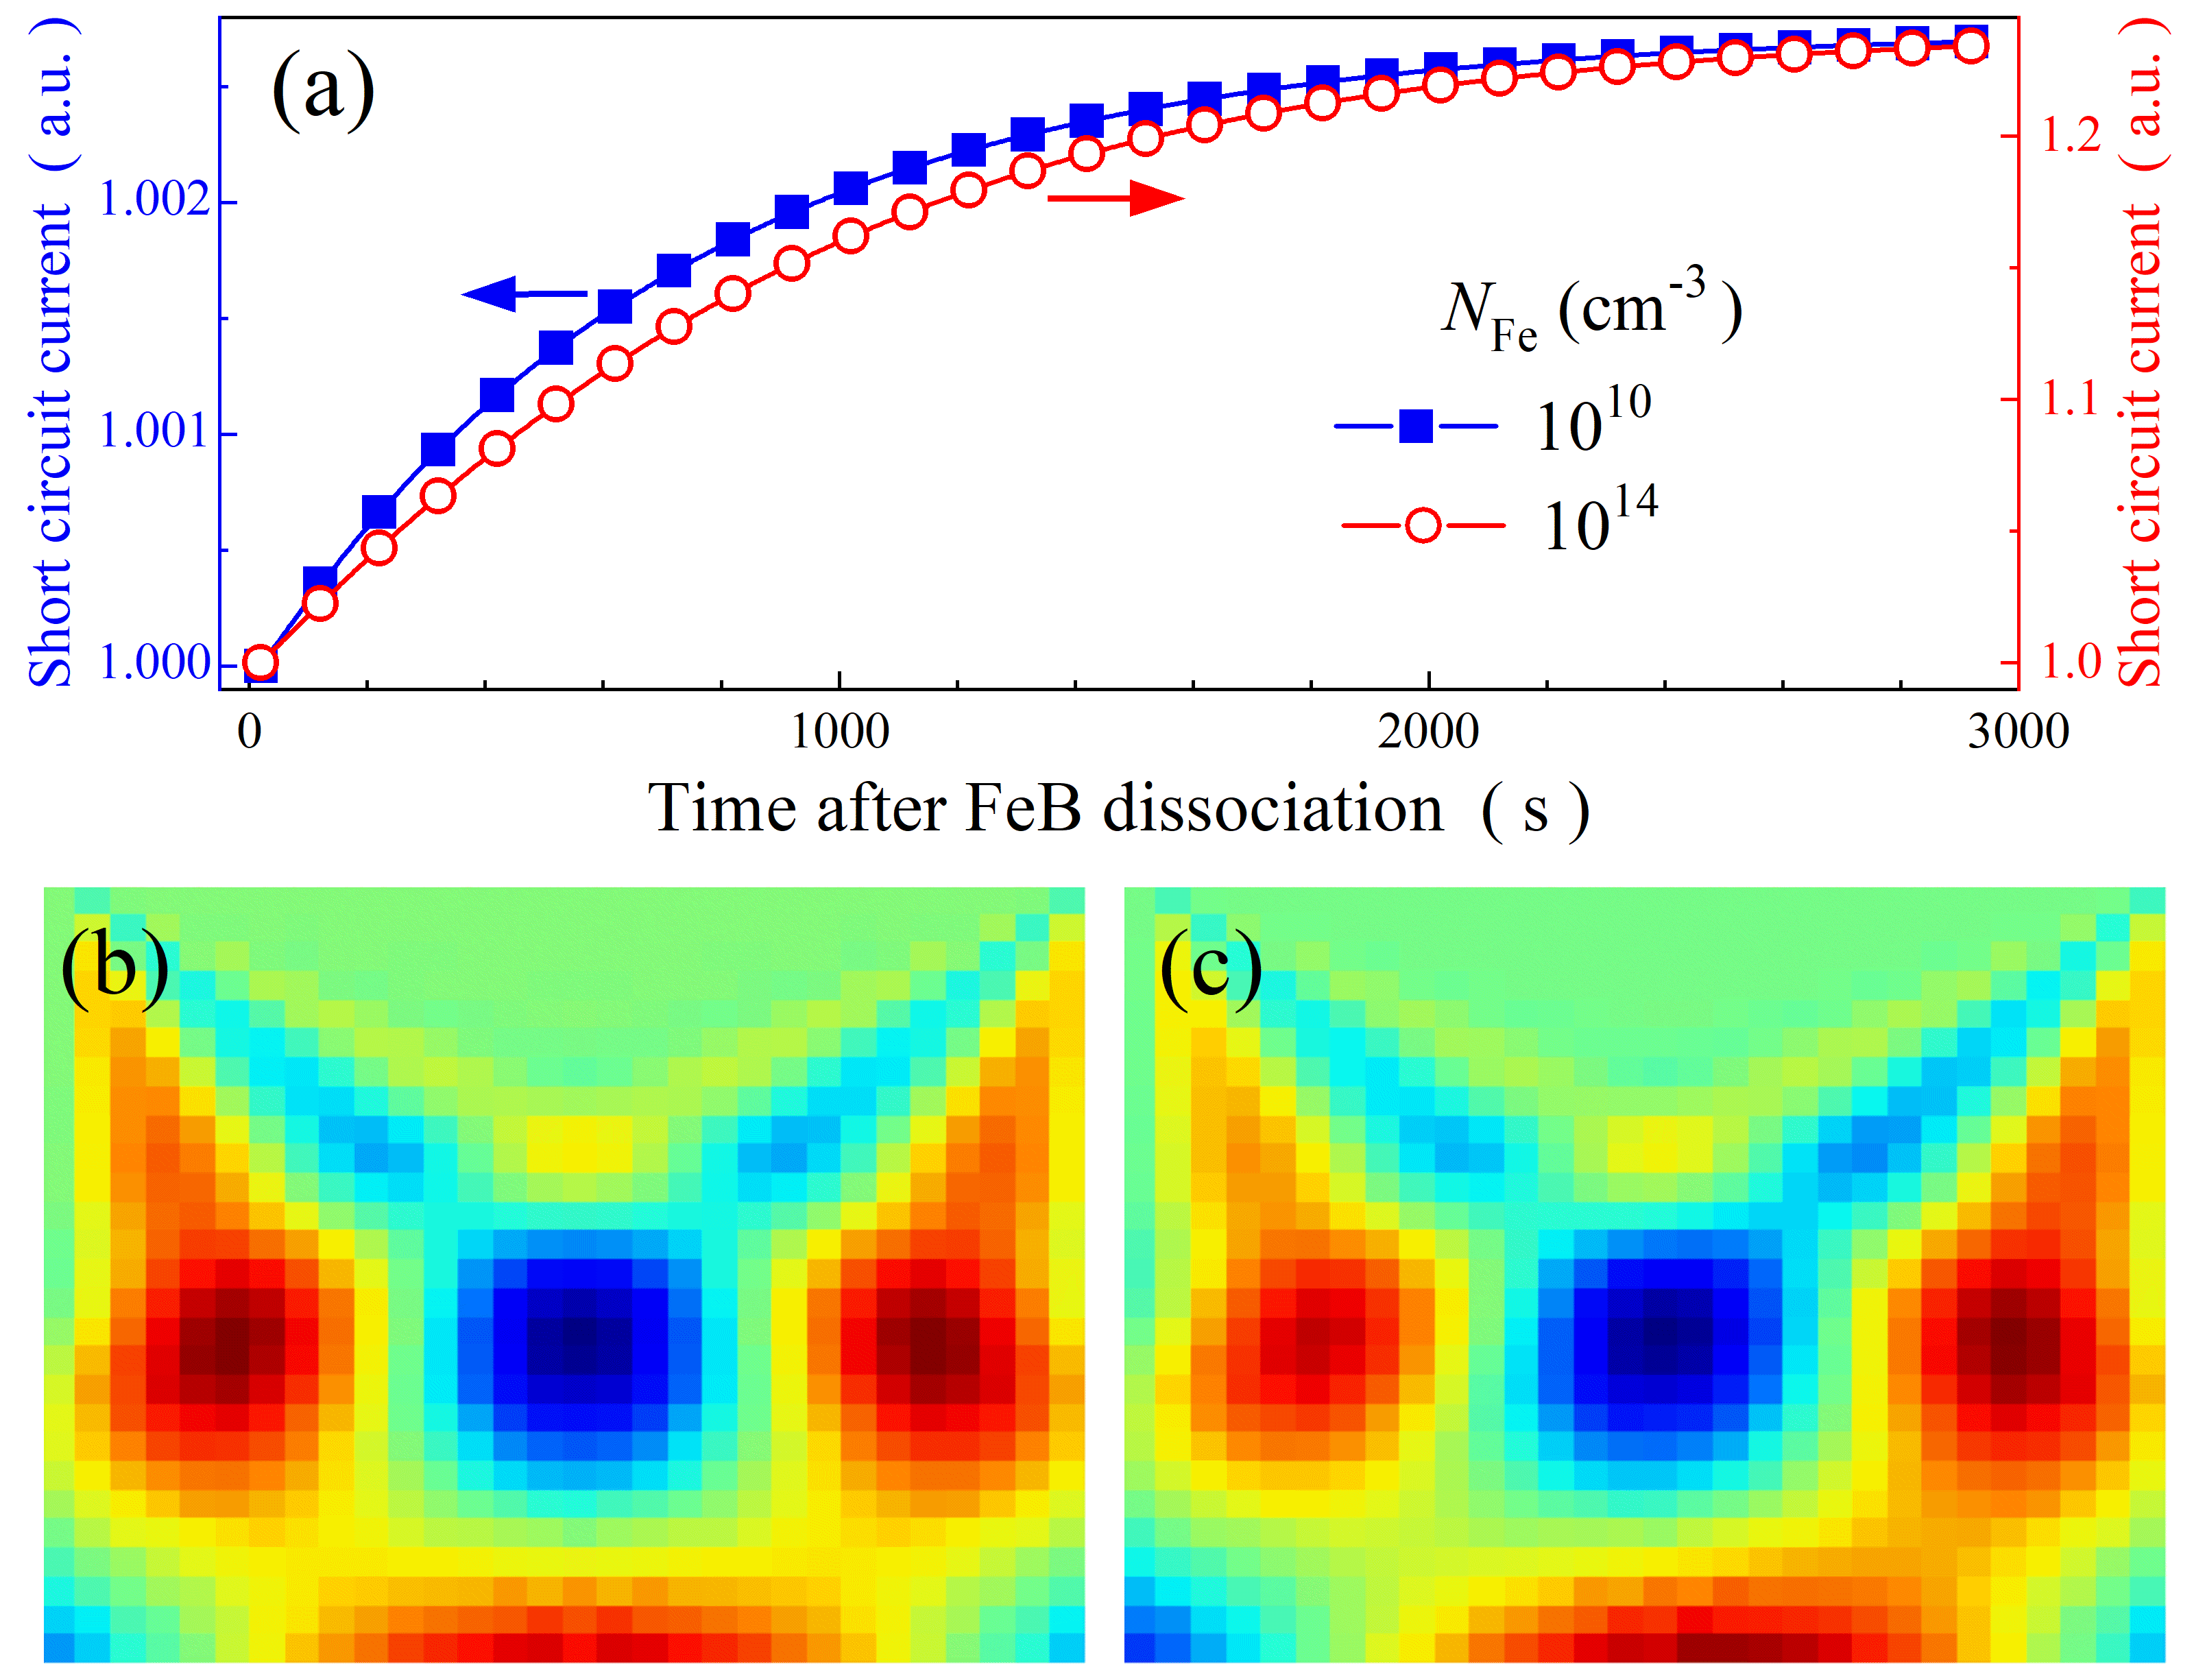
\includegraphics[width=0.5\textwidth]{Fig2}
\caption{\label{Fig2}
Simulated time dependencies of the short-circuit current (a)
and the corresponding wavelet spectrograms for iron concentrations
of $10^{10}$~cm$^{-3}$ (b) and $10^{14}$~cm$^{-3}$ (c).
The data in panel a are shown with filled squares for the concentration corresponding to panel b
and with open circles for that corresponding to panel c.
}%
\end{figure}


During the CNN Feature Processing stage, all images (both original and augmented) were processed using one of the standard CV models
to extract a feature set for each image.
The selected models and feature extraction settings are described in Subsection~\ref{subsec:CompVisMod}.
No CNN fine-tuning was performed; the models were used in their pre-trained form as downloaded.
In general, the dimensionality of the feature vectors obtained from CNN outputs substantially exceeds the number of available samples,
implying a high degree of redundancy.
Therefore, to enable comparison and mitigate this effect, Principal Component Analysis (PCA) was applied in some cases
to reduce the feature dimensionality with negligible loss of total variance.


The obtained feature sets served as inputs to regression models based on one of the standard algorithms described in Subsection~\ref{subsec:RegAlg},
which aimed to predict the iron concentration ($N_\mathtt{Fe}$) in the solar cell.
In the first case, the regression models were trained on a simulated training dataset and tested on both the simulated test dataset and experimental data.
In the second case, a portion of the experimental results was used for training, while the remaining part was reserved for testing the corresponding models.
During training, feature sets derived from the original wavelet spectrograms and their augmented versions were treated as separate samples.
During testing, the median of the predicted values obtained from the original and augmented images was used as the final prediction.
Model performance was evaluated using the metrics described in Subsection~\ref{subsec:ModEva}.


\subsection{Simulation details}\label{subsec:SimDet}

To obtain the $I_\mathtt{SC}(t)$ dependencies, $I$-$V$ curve simulations were performed for a silicon $n^+$-$p$-$p^+$ structure
under monochromatic illumination using SCAPS-1D version 3.3.11.
The SCAPS-1D software \cite{SCAPS1} is a widely used tool for modeling solar cells
while accounting for defect states \cite{MasumMia2025, Joshi2024, Ravidas2024, Liu2024, You2023, SCAPSDefect3}.
$I_\mathtt{SC}$ values were extracted from the simulated $I$-$V$ curves using a standard procedure \cite{SCparam2017}.

During the simulations, the base thickness of the structure was set to 380~$\mu$m,
and boron was used as the doping element with a concentration of $N_\mathrm{B} = 1.36 \times 10^{15}$ cm$^{-3}$.
The temperature was maintained at 340~K, and monochromatic illumination with a wavelength of  940~nm and an intensity of 5~W/m$^{2}$
was applied, corresponding to the experimental conditions (see Subsection~\ref{subsec:ExpDet}).
One of the modeling parameters was the total concentration of iron impurity atoms, $N_\mathtt{Fe}$.
It was assumed that Fe atoms were uniformly distributed throughout the base and $p^+$ layer of the solar cell
and could exist either in interstitial positions, with a concentration $N_\mathtt{Fe_i}$, or as FeB pairs, with a concentration $N_\mathtt{FeB}$.
The time dependence of $N_\mathtt{Fe_i}$ after pair dissociation follows the well-known expression \cite{MurphyJAP2011, Wijaranakula}:
\begin{equation}
\label{eqNFet}
N_\mathrm{Fe_i}(t)=(N_\mathrm{Fe_i,0}-N_\mathrm{Fe_i,eq})\times
\exp(-t/\tau_\mathrm{ass})+N_\mathrm{Fe_i,eq}\,,
\end{equation}
where
where $N_\mathrm{Fe_i,0}$ is the concentration of interstitial iron atoms formed due to FeB pair dissosiation,
$N_\mathtt{Fe_i,0} = N_\mathtt{Fe_i}(t=0) = N_\mathtt{Fe}$;
$N_\mathtt{Fe_i,eq}$ is the portion of interstitial iron atoms that remain unpaired in the equilibrium state
$N_\mathtt{Fe_i,eq}=N_\mathtt{Fe_i}(t \rightarrow \infty)$,
according to \cite{MurphyJAP2011, Wijaranakula}
\begin{equation}\label{eqFeieq}
  N_\mathtt{Fe_i,eq}=\frac{N_\mathtt{Fe}}{\left[1+N_\mathtt{B}\cdot A_z \cdot \exp\left(\frac{E_b}{kT}\right)\right]
  \left[1+\exp\left(\frac{E_F-E_\mathtt{Fe_i}}{kT}\right)\right]}\,,
\end{equation}
$E_b$ is the binding energy of the FeB pairs (taken as 0.582~eV \cite{Wijaranakula}),
$A_z $ depends on the number of possible orientations of the pair and lattice site density
(taken as $10^{-23}$~cm$^3$ \cite{MurphyJAP2011}),
$E_F$ is the Fermi level,
$E_\mathtt{Fe_i}$ is the position of the donor Fe$_i$ level relative to the valence band maximum
(taken as 0.394~eV \cite{FeBAssJAP2014});
$\tau_\mathrm{ass}$ is the characteristic time of the complex association,
according to \cite{FeBKin2019,FeBAssJAP2014,FeBAssSST2011}
\begin{equation}
\label{eqTass}
\tau_\mathrm{ass}=A\times\frac{T}{N_A}\exp\left(\frac{E_m}{kT}\right)\,,
\end{equation}
$E_m$ is the energy of Fe$_\mathtt{i}^+$ migration (taken as 0.66~eV \cite{FeBAssJAP2014,FeBKin2019,FeBAssSST2011}),
$A$ is the constant (taken as $5.7\times10^5\,\frac{\mathrm{s}}{\mathrm{K}\;\mathrm{cm}^3}$ \cite{FeBAssSST2011}).
In its turn, the iron–boron pair concentration $N_\mathtt{FeB}$, was estimated from
\begin{equation}\label{eqNFeB}
  N_\mathtt{FeB}(t)+N_\mathtt{Fe_i}(t)=N_\mathtt{Fe}\,.
\end{equation}
Overall, the concentrations of iron-related defects depended not only on time but
also on their spatial position within the structure, reflecting the non-uniformity of the $(E_F-E_\mathtt{Fe_i})$ difference.

A detailed description of the modeling approach, including the values of silicon and defect parameters employed, is provided elsewhere \cite{Olikh2025MSEB, Olikh2019SM}.

To create the training dataset, 25 $N_\mathtt{Fe}$ values were selected, evenly distributed on a logarithmic scale from $10^{10}$~cm$^{-3}$ to $10^{14}$~cm$^{-3}$.
Examples of the resulting dependencies are shown in \Fref{Fig2}, along with the corresponding wavelet spectrograms.
The simulated test dataset consisted of 10 dependencies calculated for 10 $N_\mathtt{Fe}$ values not included in the training dataset.



\subsection{Experiment details}\label{subsec:ExpDet}

The proposed method was validated using measurements of $n^+$-$p$-$p^+$ silicon solar cells fabricated on
380~$\mu$m thick $p$-type boron-doped Cz wafers ($N_\mathrm{B}=1.36\times10^{15}$~cm$^{-3}$).
The $n^+$ (0.7~$\mu$m, 20–30 $\Omega$/$\Box$) and $p^+$ (0.6~$\mu$m, 10–20 $\Omega$/$\Box$)
layers were formed by phosphorus and boron diffusion, respectively.
Details of the fabrication procedure are provided elsewhere \cite{Olikh2021JAP}.

Current–voltage curves and $I_\mathtt{SC}$ kinetics were measured with a Keithley 2450 source meter.
A 940~nm SN-HPIR940nm-1W LED (intensity 5 W/m$^{2}$) served as a monochromatic light source,
with its output stabilized by a W1209 thermostat and a feedback-controlled power supply.
The cell temperature was regulated by a thermoelectric cooler with an STS-21 sensor and maintained constant by a PID algorithm in the control software.
FeB-pair dissociation was induced by intense (about 7000~W/m$^{2}$) halogen-lamp illumination.
The illumination intervals were selected according to a previous study \cite{OlikhPSSA}.
The kinetics of the short-circuit current were measured in the dark at 340~K for 3000~s.
According to Eq.~\eref{eqTass}, this interval is sufficient for the complete restoration of the iron–boron pairs to their equilibrium concentration.


\Fref{Fig3}a presents an example of a measured $I_\mathtt{SC}$(t) dependence.
The signal contains some noise because, despite using a thermostat, the LED temperature fluctuated by approximately 0.4~K.
A Savitzky–Golay filter was applied for smoothing, with the window lengths and filter order selected adaptively ccording to Krishnan and Seelamantula \cite{Krishnan2013}.
Only current values corresponding to the time points used in the simulations were retained for the wavelet transformation.
The smoothed curve is shown in \Fref{Fig3}a,
while the remaining panels of the figure display the spectrograms obtained from the raw experimental curve and the processed dependence.

\begin{figure}
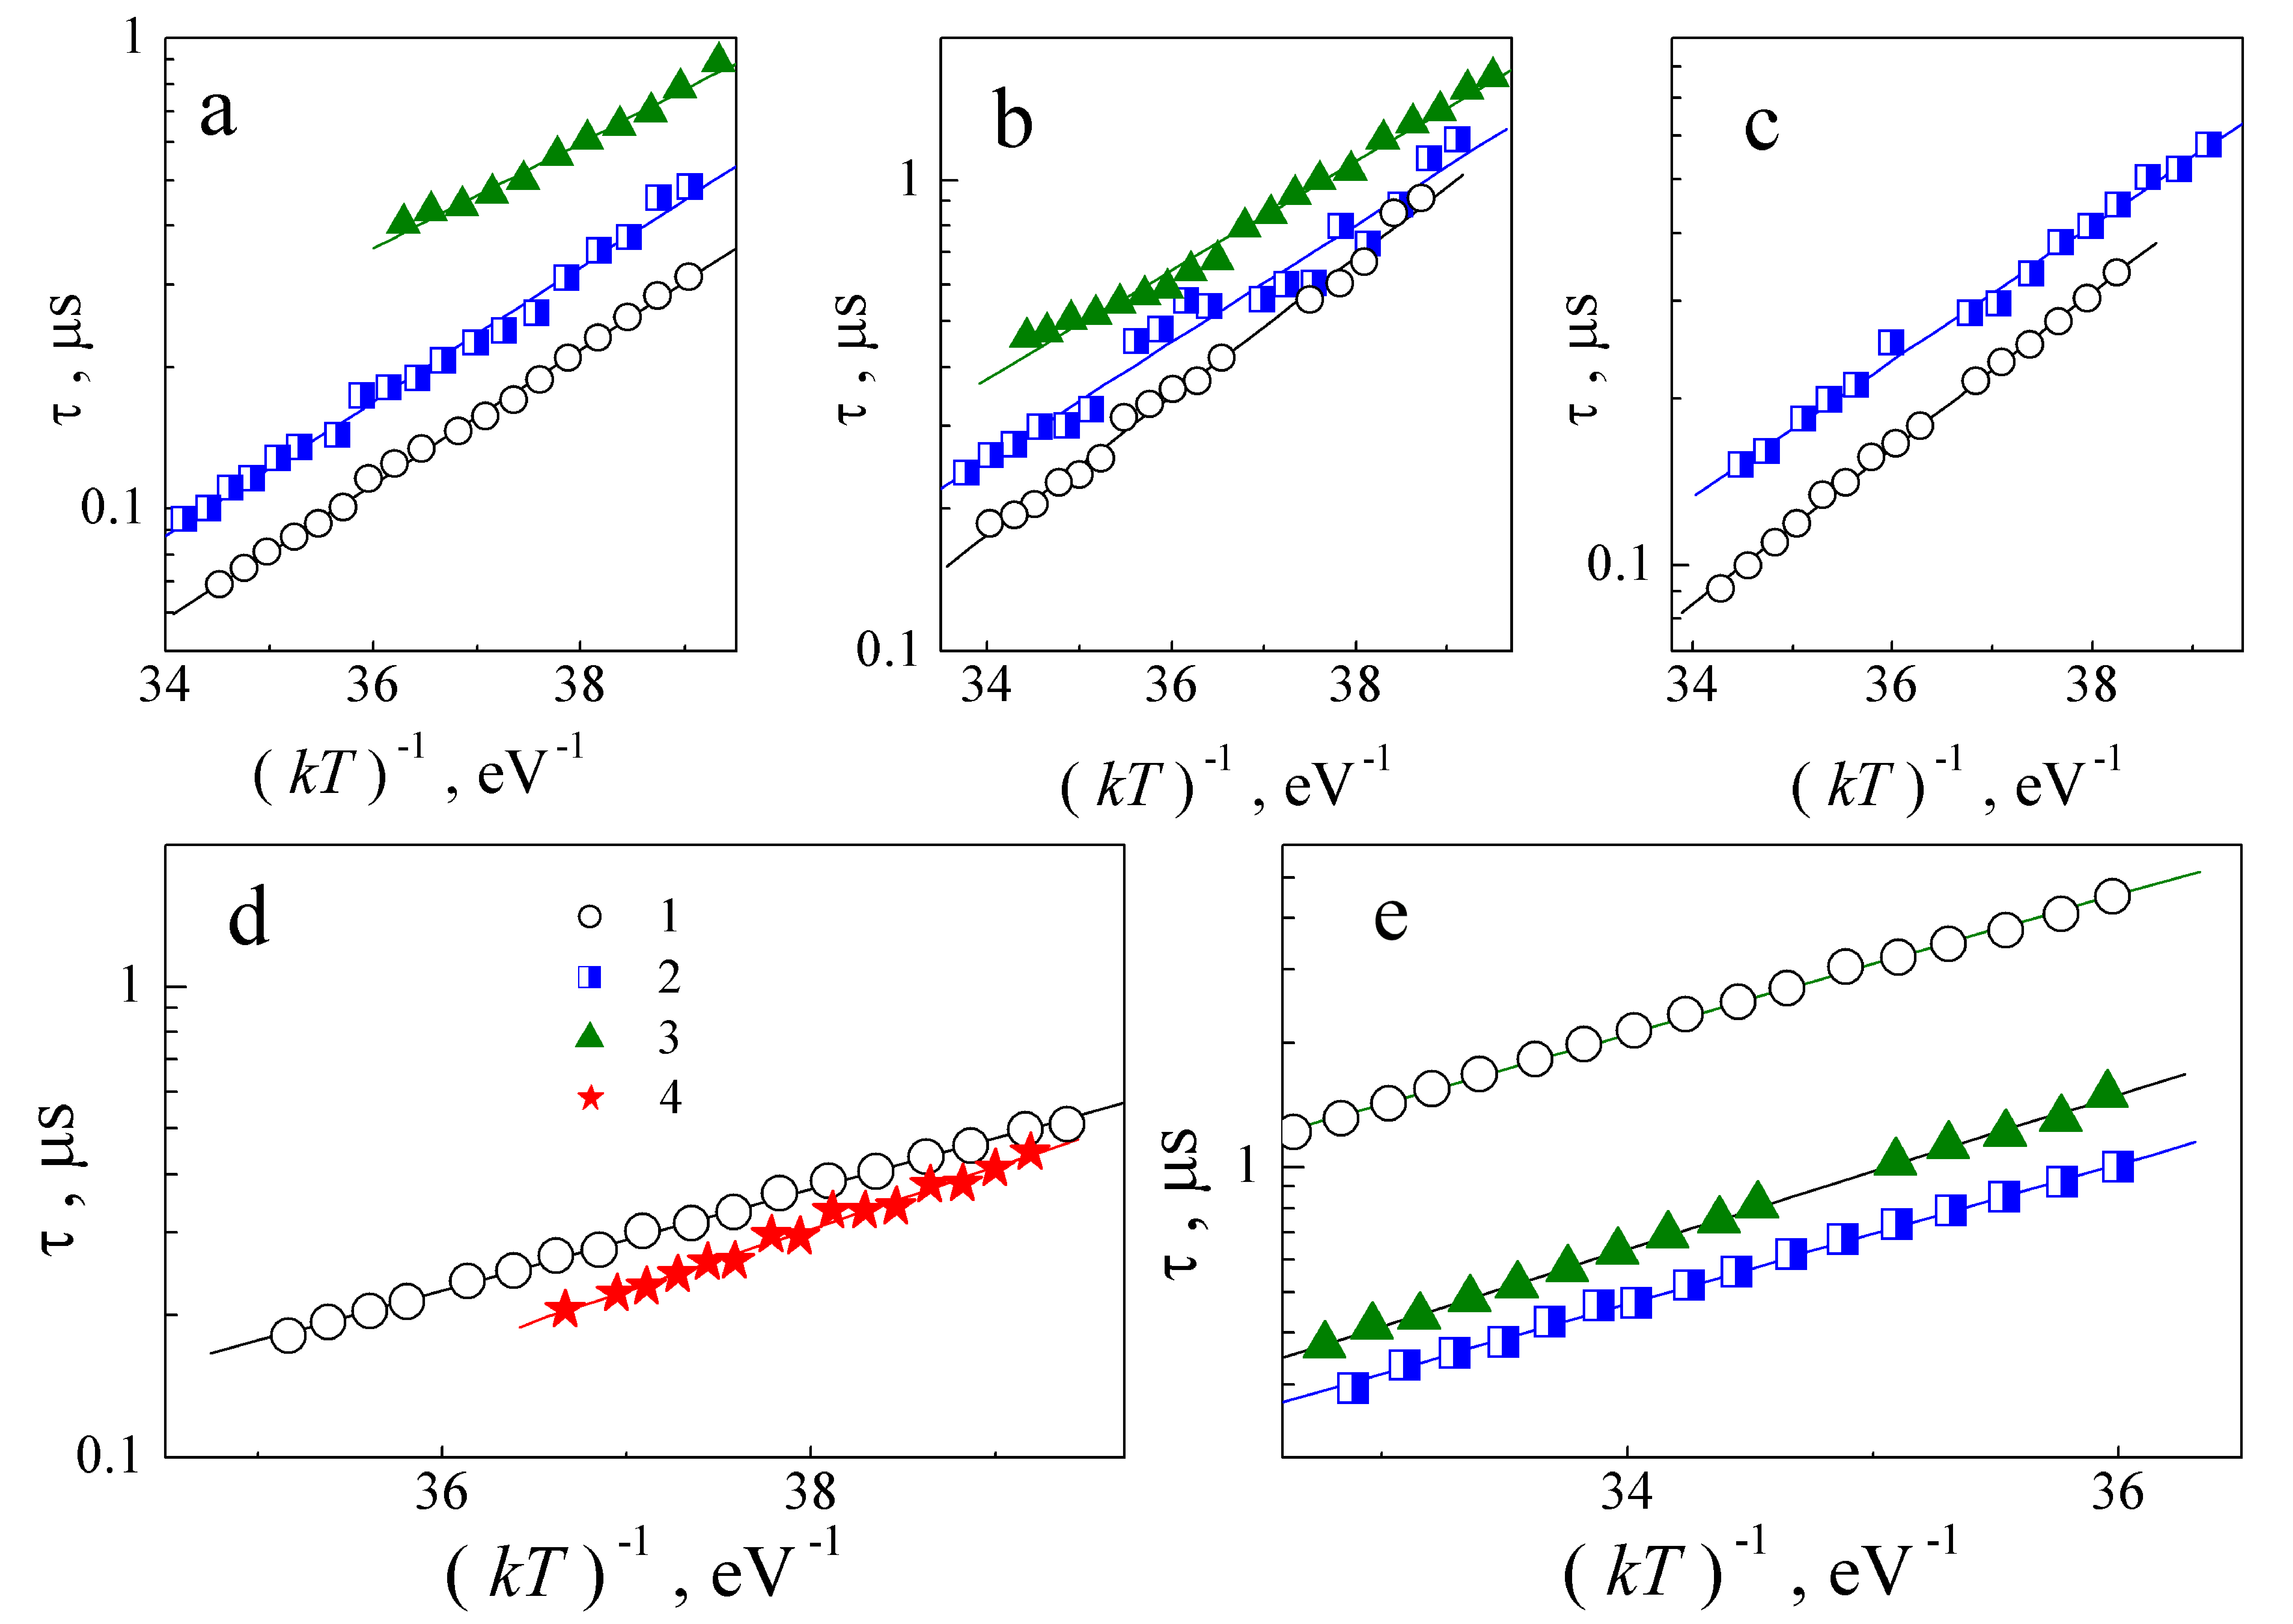
\includegraphics[width=0.5\textwidth]{Fig3}
\caption{\label{Fig3}
(a) Experimentally measured time dependence of the short-circuit current for a sample with
$N_\mathtt{Fe}=2.8\cdot10^{13}$~cm$^{-3}$ (a, open  squares) and the same dependence after applying the Savitzky–Golay filter (filled circles).
Panels (b) and (c) show the wavelet spectrograms corresponding to the curves with filled squares and open circles, respectively.
}%
\end{figure}

The iron concentration $N_\mathtt{Fe}$ was determined using a methodology described in \cite{Olikh2022:JMatSci,Olikh2021JAP},
which is based on fitting the kinetics of the short circuit current following FeB pairs dissociation.
A total of 28 samples with iron concentrations ranging from $10^{11}$~cm$^{-3}$ to $2\times10^{13}$~cm$^{-3}$ were examined.
To evaluate models trained on simulated data, the entire experimental dataset was used as the test set.
In cases where the models were trained using experimental data, 20 randomly selected samples were included in the training set,
while the remaining eight samples were used for testing.



\subsection{Computer vision models}\label{subsec:CompVisMod}

To extract graphical features from the wavelet spectrograms, several computer vision models available in Keras were employed,
namely EfficientNetB7, ResNet152V2, MobileNetV2, Xception, and NASNetLarge.
Although these models have different architectures, they all belong to the CNN class, are designed for object classification,
and have previously been applied successfully to processing EL images of solar cells \cite{Jia2024, Otamendi2021, Chen2022, Abdelsattar2025, tella2025}.
Two feature extraction strategies were evaluated for all models:
in the first, the class-specific probability distributions (soft labels) were passed to the subsequent stage of the pipeline,
while in the second, the raw feature vectors directly extracted by the computer vision model were utilized.

Furthermore, the CSPDarknet53 model was employed,
which serves as the CNN backbone for YOLOv4.
Models of this family feature a more sophisticated CNN architecture optimized not for single-object classification
but for multi-object detection in images.
They are widely used in imaging-based techniques \cite{Liu2024a, Li2024a, Chen2022}.
The employed model produces three feature maps, and for subsequent processing, either only the highest-level layer or the two deepest layers were selected.

It is well known that increasing the feature dimensionality does not necessarily enhance the total information variance.
To mitigate the impact of redundant data, Principal Component Analysis (PCA) was applied, which constructs new, uncorrelated features (principal components).
PCA is a widely used and effective technique in machine learning, particularly for improving performance in Electrical Testing Techniques \cite{Fadhel2019, Gao2020}.
In this study, PCA was applied to the training datasets with an explained variance threshold of 99.9\%.
In other words, the principal components explaining no less than 99.9\% of the total variance in the original features were selected,
thus achieving a substantial reduction in feature dimensionality.
This pre-processing procedure was selectively applied to a subset of the computer vision models ---
specifically, those demonstrating good performance on the test sets without PCA --- with the aim of assessing the feasibility and effectiveness of this approach.

Given the remarkably high dimensionality of the features produced by YOLOv4,
the feasibility of applying an alternative dimensionality reduction technique was examined.
Specifically, global average pooling was applied to each convolutional feature map,
replacing the spatial map with its mean value and thereby yielding a single scalar value per channel.

The configurations of the computer vision models used in this study are summarized in \tref{tabUsedMod}.
The table also lists the notations that are subsequently used to refer to these configurations.


\begin{table*}
\centering
\caption{Summary of used pretrained CV models and feature extraction variants \label{tabUsedMod}}
\begin{indented}
\item[]
\begin{tabular}{p{2.5cm}p{4.5cm}ccc}
\br
Base model &   Model type &   Feature processing &   Output dimension &   Model Label \\
\mr
EfficientNetB7 & Classifier        & None & 1000 & ENB7:CL   \\
               & Feature extractor & None & 2560 & ENB7:FE   \\
               &                   & PCA  & 39   & ENB7:FE:P \\
MobileNetV2    & Classifier        & None & 1000 & MNV2:CL   \\
               & Feature extractor & None & 1280 & MNV2:FE   \\
               &                   & PCA  & 124  & MNV2:FE:P \\
NASNetLarge    & Classifier        & None & 1000 & NAS:CL    \\
               &                   & PCA  & 30   & NAS:CL:P  \\
               & Feature extractor & None & 4032 & NAS:FE    \\
ResNet152V2    & Classifier        & None & 1000 & R152:CL   \\
               & Feature extractor & None & 2048 & R152:FE   \\
Xception       & Classifier        & None & 1000 & XCP:CL    \\
               & Feature extractor & None & 2048 & XCP:FE    \\
YOLOv4 \newline (CSPDarknet53)&  Feature extractor  \newline (raw, top layer)& None &86528 &  YL:FE1 \\
&&PCA  & 137  & YL:FE1:P  \\
&Feature extractor  \newline (raw, top \& penultimate layers)&None &  433640 &  YL:FE2 \\
&&PCA  & 142  & YL:FE2:P  \\
&Feature extractor \newline (pooled, top layer)&None &  512 &  YL:FP1 \\
&Feature extractor \newline (pooled, top \& penultimate layers)& None &  1024 &  YL:FP2 \\
\br
\end{tabular}
\end{indented}
\end{table*}

\subsection{Regression algorithms}\label{subsec:RegAlg}

Five ML algorithms were employed to develop regression models for predicting iron concentration:
Random Forest (RF), Gradient Boosting (GB), eXtreme Gradient Boosting (XGB), Support Vector Regression (SVR), and Deep Neural Network (DNN).
The models were implemented using Python libraries: Keras for DNN, Scikit-learn for RF, GB, and SVR, and XGBoost for XGB.

Each regression model was trained using features obtained from all configurations listed in \tref{tabUsedMod} and subsequently used to make predictions.
The only exception involved the uncompressed features extracted by YOLOv4, for which the available computational resources
(2.9 GHz AMD Ryzen 7 4800H CPU, 8 GB RAM, GeForce GTX 1650 4 GB) permitted the use of SVR only.
The target variable of all models was $\log N_\mathtt{Fe}$.
Such logarithmic transformation is a standard approach for achieving higher prediction accuracy
when the target quantity spans several orders of magnitude \cite{Srivastava2023, Minagawa2024}.
Both input features and target values were normalized to have zero mean and unit standard deviation within the training set.

For each scenario, regression models were optimized to enhance predictive performance.
Hyperparameter tuning was performed using the Optuna toolkit,
employing the TPE sampler and the Hyperband pruner to ensure efficient selection.
The complete list of tuned hyperparameters and their respective search ranges is provided in Tables~S1–S5 (Supplementary Material).
Five-fold cross-validation was implemented during model tuning, with 20\% of the training data used as a validation set
to evaluate models trained on the remaining 80\%.
The resulting optimal hyperparameter combinations are presented in Tables~S6–S10.

Consequently, 87 distinct combinations of computer vision and regression models were investigated.
Each combination was subsequently trained and evaluated using both simulated and experimental data.
To identify the results for each case, a composite label was employed, derived from the last column of \tref{tabUsedMod}
and the abbreviated name of the regression algorithm.


\subsection{Model evaluation}\label{subsec:ModEva}

A rigorous assessment of model performance across diverse metrics is essential for constructing a robust regression model.
The evaluation metrics for iron quantification were the mean squared error (MSE),
mean absolute percentage error (MAPE),
median absolute percentage error (MedAPE) and
coefficient of determination (R$^2$), as defined in Eqs.~\eref{eqMSE}-\eref{eqR2}.
\begin{equation}\label{eqMSE}
  \mathtt{MSE} = \frac{1}{N}\sum_{i=1}^{N} (\hat{y_i}-y_i)^2\,,
\end{equation}
\begin{equation}\label{eqMAPE}
  \mathtt{MAPE} = \frac{1}{N}\sum_{i=1}^{N} \mathtt{MAPE}_i\,,
\end{equation}
\begin{equation}\label{eqMAPEi}
  \mathtt{MAPE}_i = \frac{|N_{\mathrm{Fe,PRED},i}-N_{\mathrm{Fe,TRUE},i}|}{N_{\mathrm{Fe,TRUE},i}}\times 100 \%\,,
\end{equation}
\begin{equation}\label{eqMedAPE}
  \mathtt{MedAPE} = \frac{1}{2} \left[\mathtt{MAPE}_{\lceil\frac{N}{2}\rceil}+\mathtt{MAPE}_{\lfloor\frac{N}{2}+1\rfloor}\right]\,,
\end{equation}
\begin{equation}\label{eqR2}
  R^2 = 1-\frac{\displaystyle\sum_{i=1}^{N} (N_{\mathrm{Fe,TRUE},i}-N_{\mathrm{Fe,PRED},i})^2}{\displaystyle\sum_{i=1}^{N} (N_{\mathrm{Fe,TRUE},i}-\overline{{N_\mathrm{Fe,TRUE}}})^2},
\end{equation}
where
where $\hat{y_i}$ is the predicted value of the target variable for the $i$-th data point,
$y_i$ is the corresponding known value (obtained by logarithmic transformation and normalization of the iron concentration);
$N$ denotes the number of samples in the dataset
($N = 25$ for the simulated training set, 20 for the experimental training set,
10 for the simulated test set,
and 28 and 8 for the experimental datasets used to test models trained on the simulated and experimental sets, respectively);
$\mathtt{MAPE}_i$ is the  absolute percentage error for $i$-th data point;
$N_{\mathrm{Fe,PRED},i}$ is the predicted iron concentration,
$N_{\mathrm{Fe,TRUE},i}$ is the known value
(either the parameter used in the simulation or obtained from experimental iron determination);
$\overline{N_\mathrm{Fe,TRUE}}$ is the mean of the true values in the dataset.

MSE is one of the most widely used metrics for evaluating model accuracy,
and the training objective was specifically defined to minimize this quantity.
However, since the computation of $y_i$ involves both normalization and a logarithmic transformation of $N_\mathtt{Fe}$,
the MSE metric alone does not fully reflect the accuracy of the iron concentration estimation.
Therefore, the MAPE, which quantifies the mean relative deviation, was also employed.
In addition, the MedAPE, representing the error value below which 50\% of the predictions fall,
provides a more robust measure against the influence of individual outliers,
which can have a particularly large effect on mean-based metrics in smaller datasets.
Finally, the $R^2$ was used to quantify the fraction of the variance in the
target variable explained by the model,
thereby indicating how well the predicted values reproduce the observed data;
a value of 1 corresponds to perfect agreement.


\section{Results and discussion}\label{sec:Rez}
\subsection{Simulated data}

\Fref{Fig4} illustrates representative prediction results obtained from models trained on the simulated training dataset.
The complete set of results, covering all 87 investigated configurations, is provided in Figure~S1 of the Supplementary Material.

%\begin{figure*}
%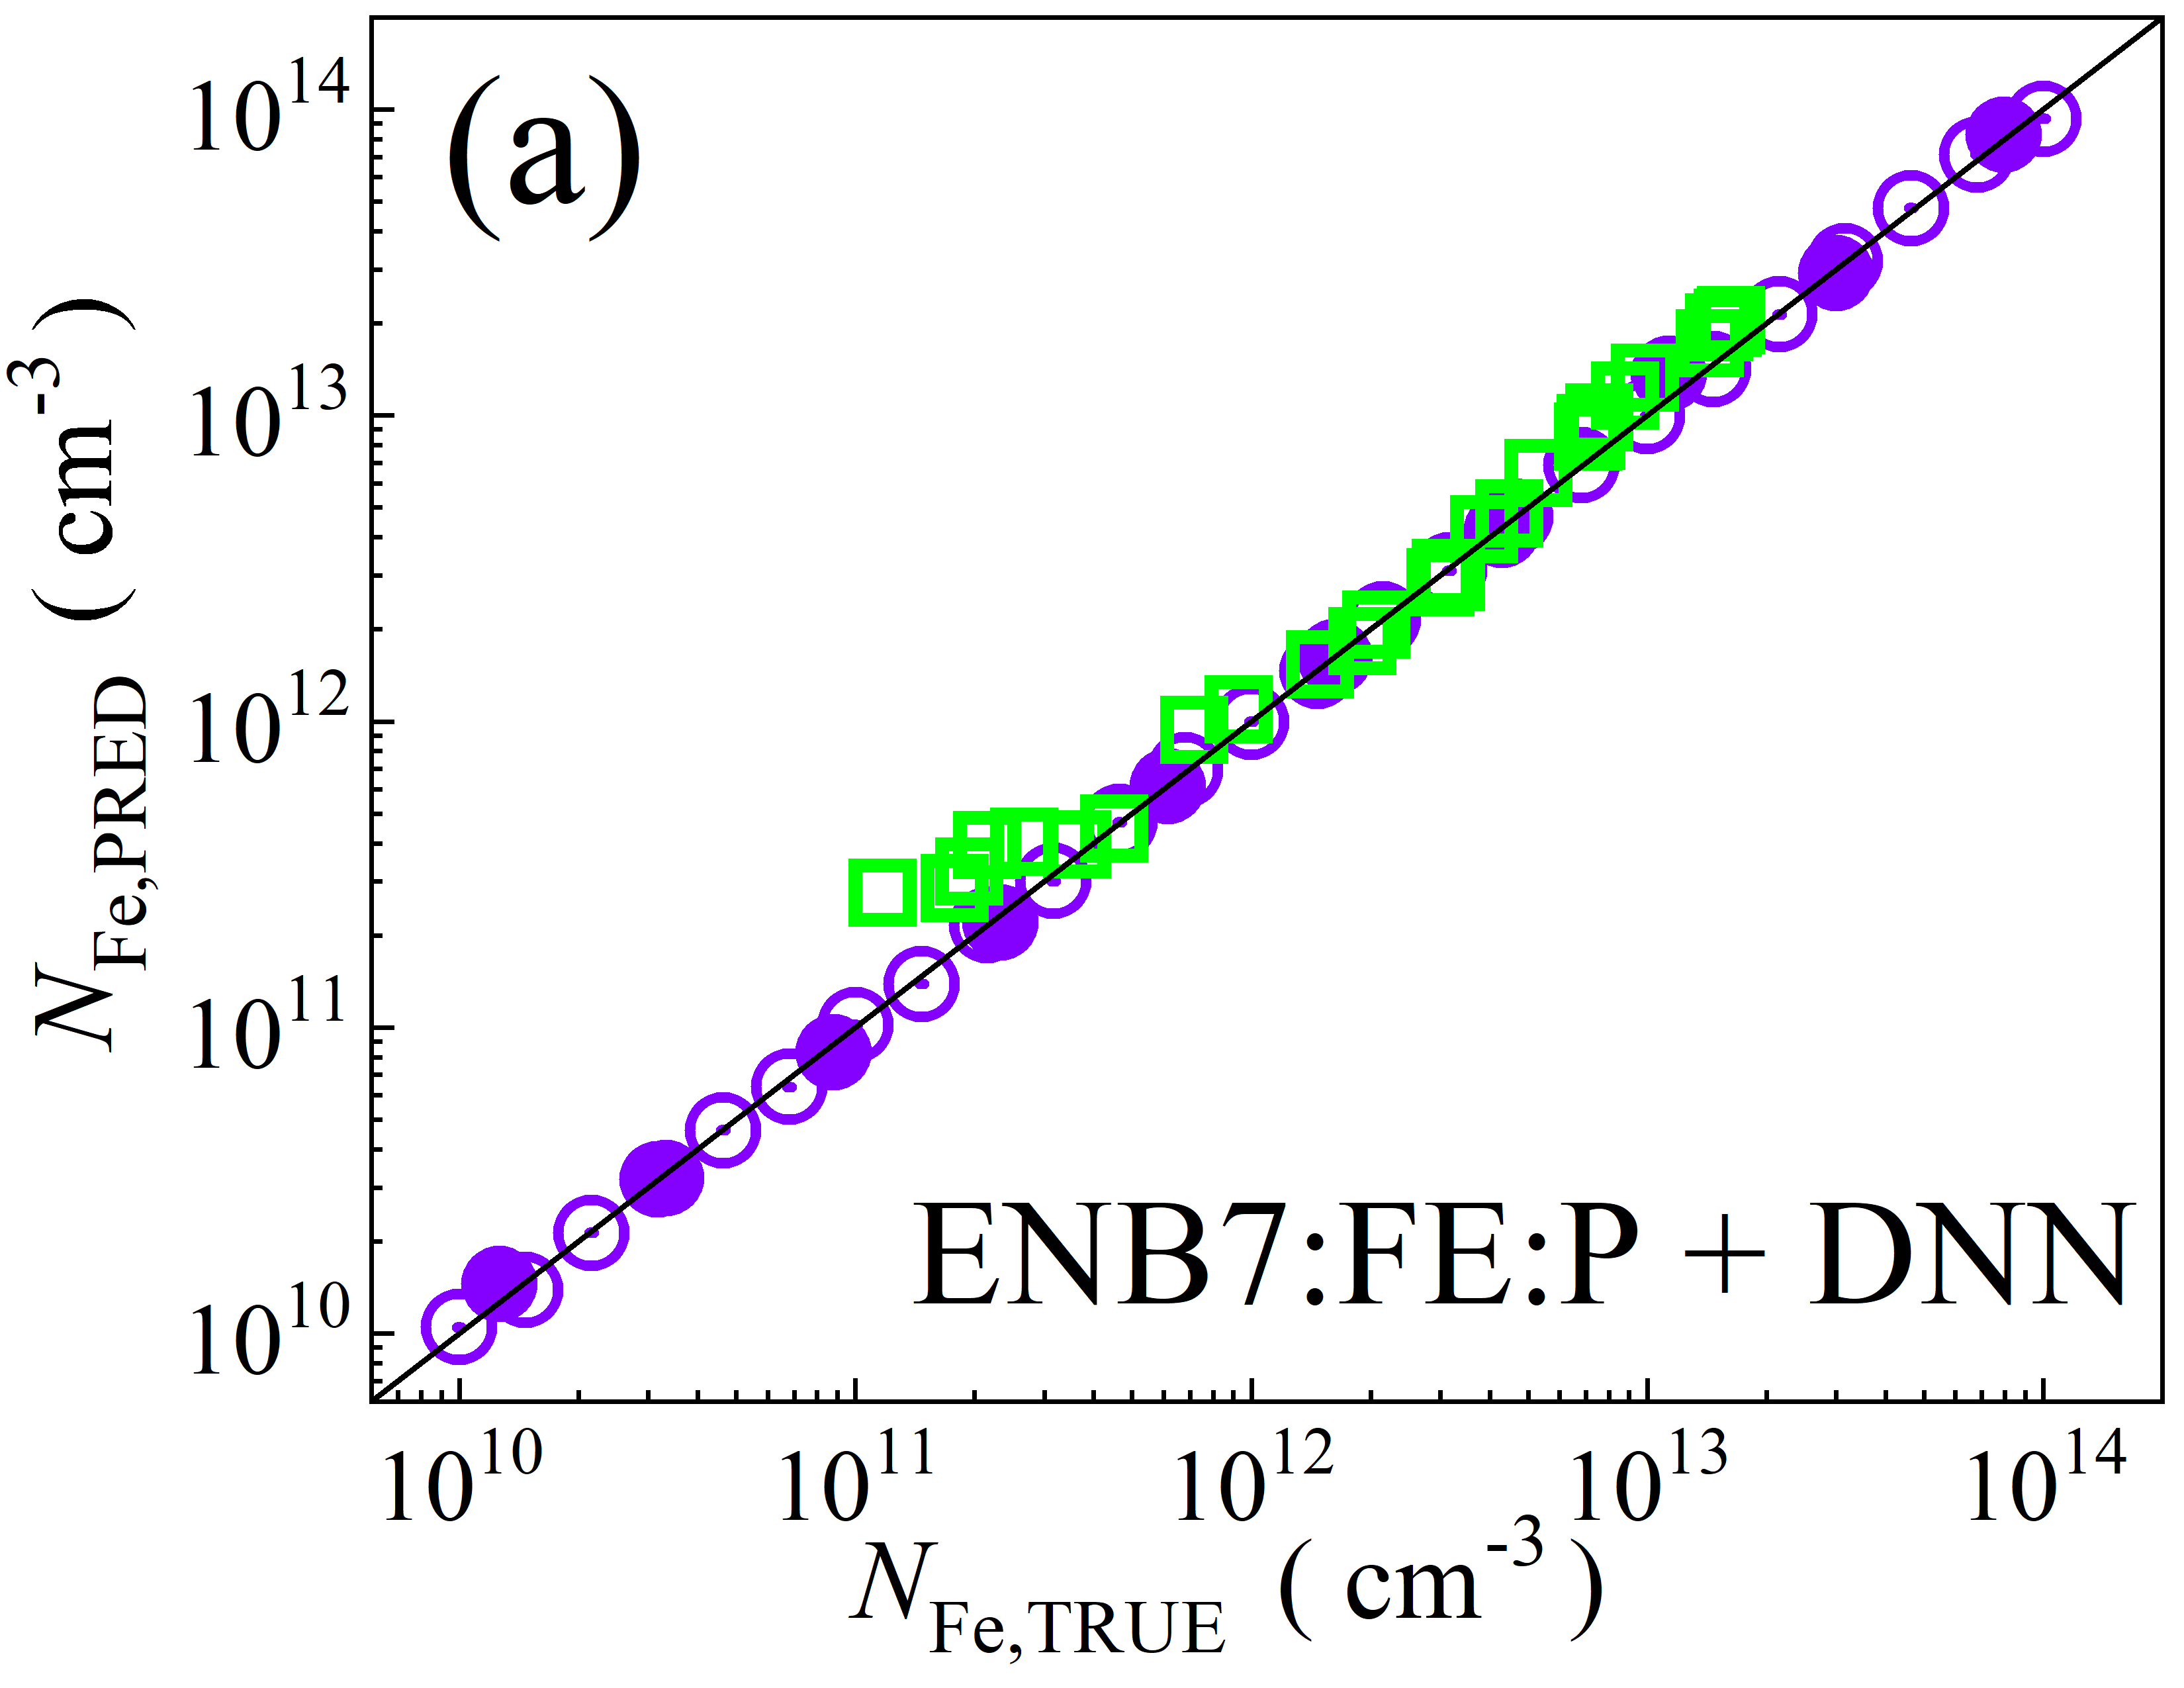
\includegraphics[width=0.24\textwidth]{Fig4a}
%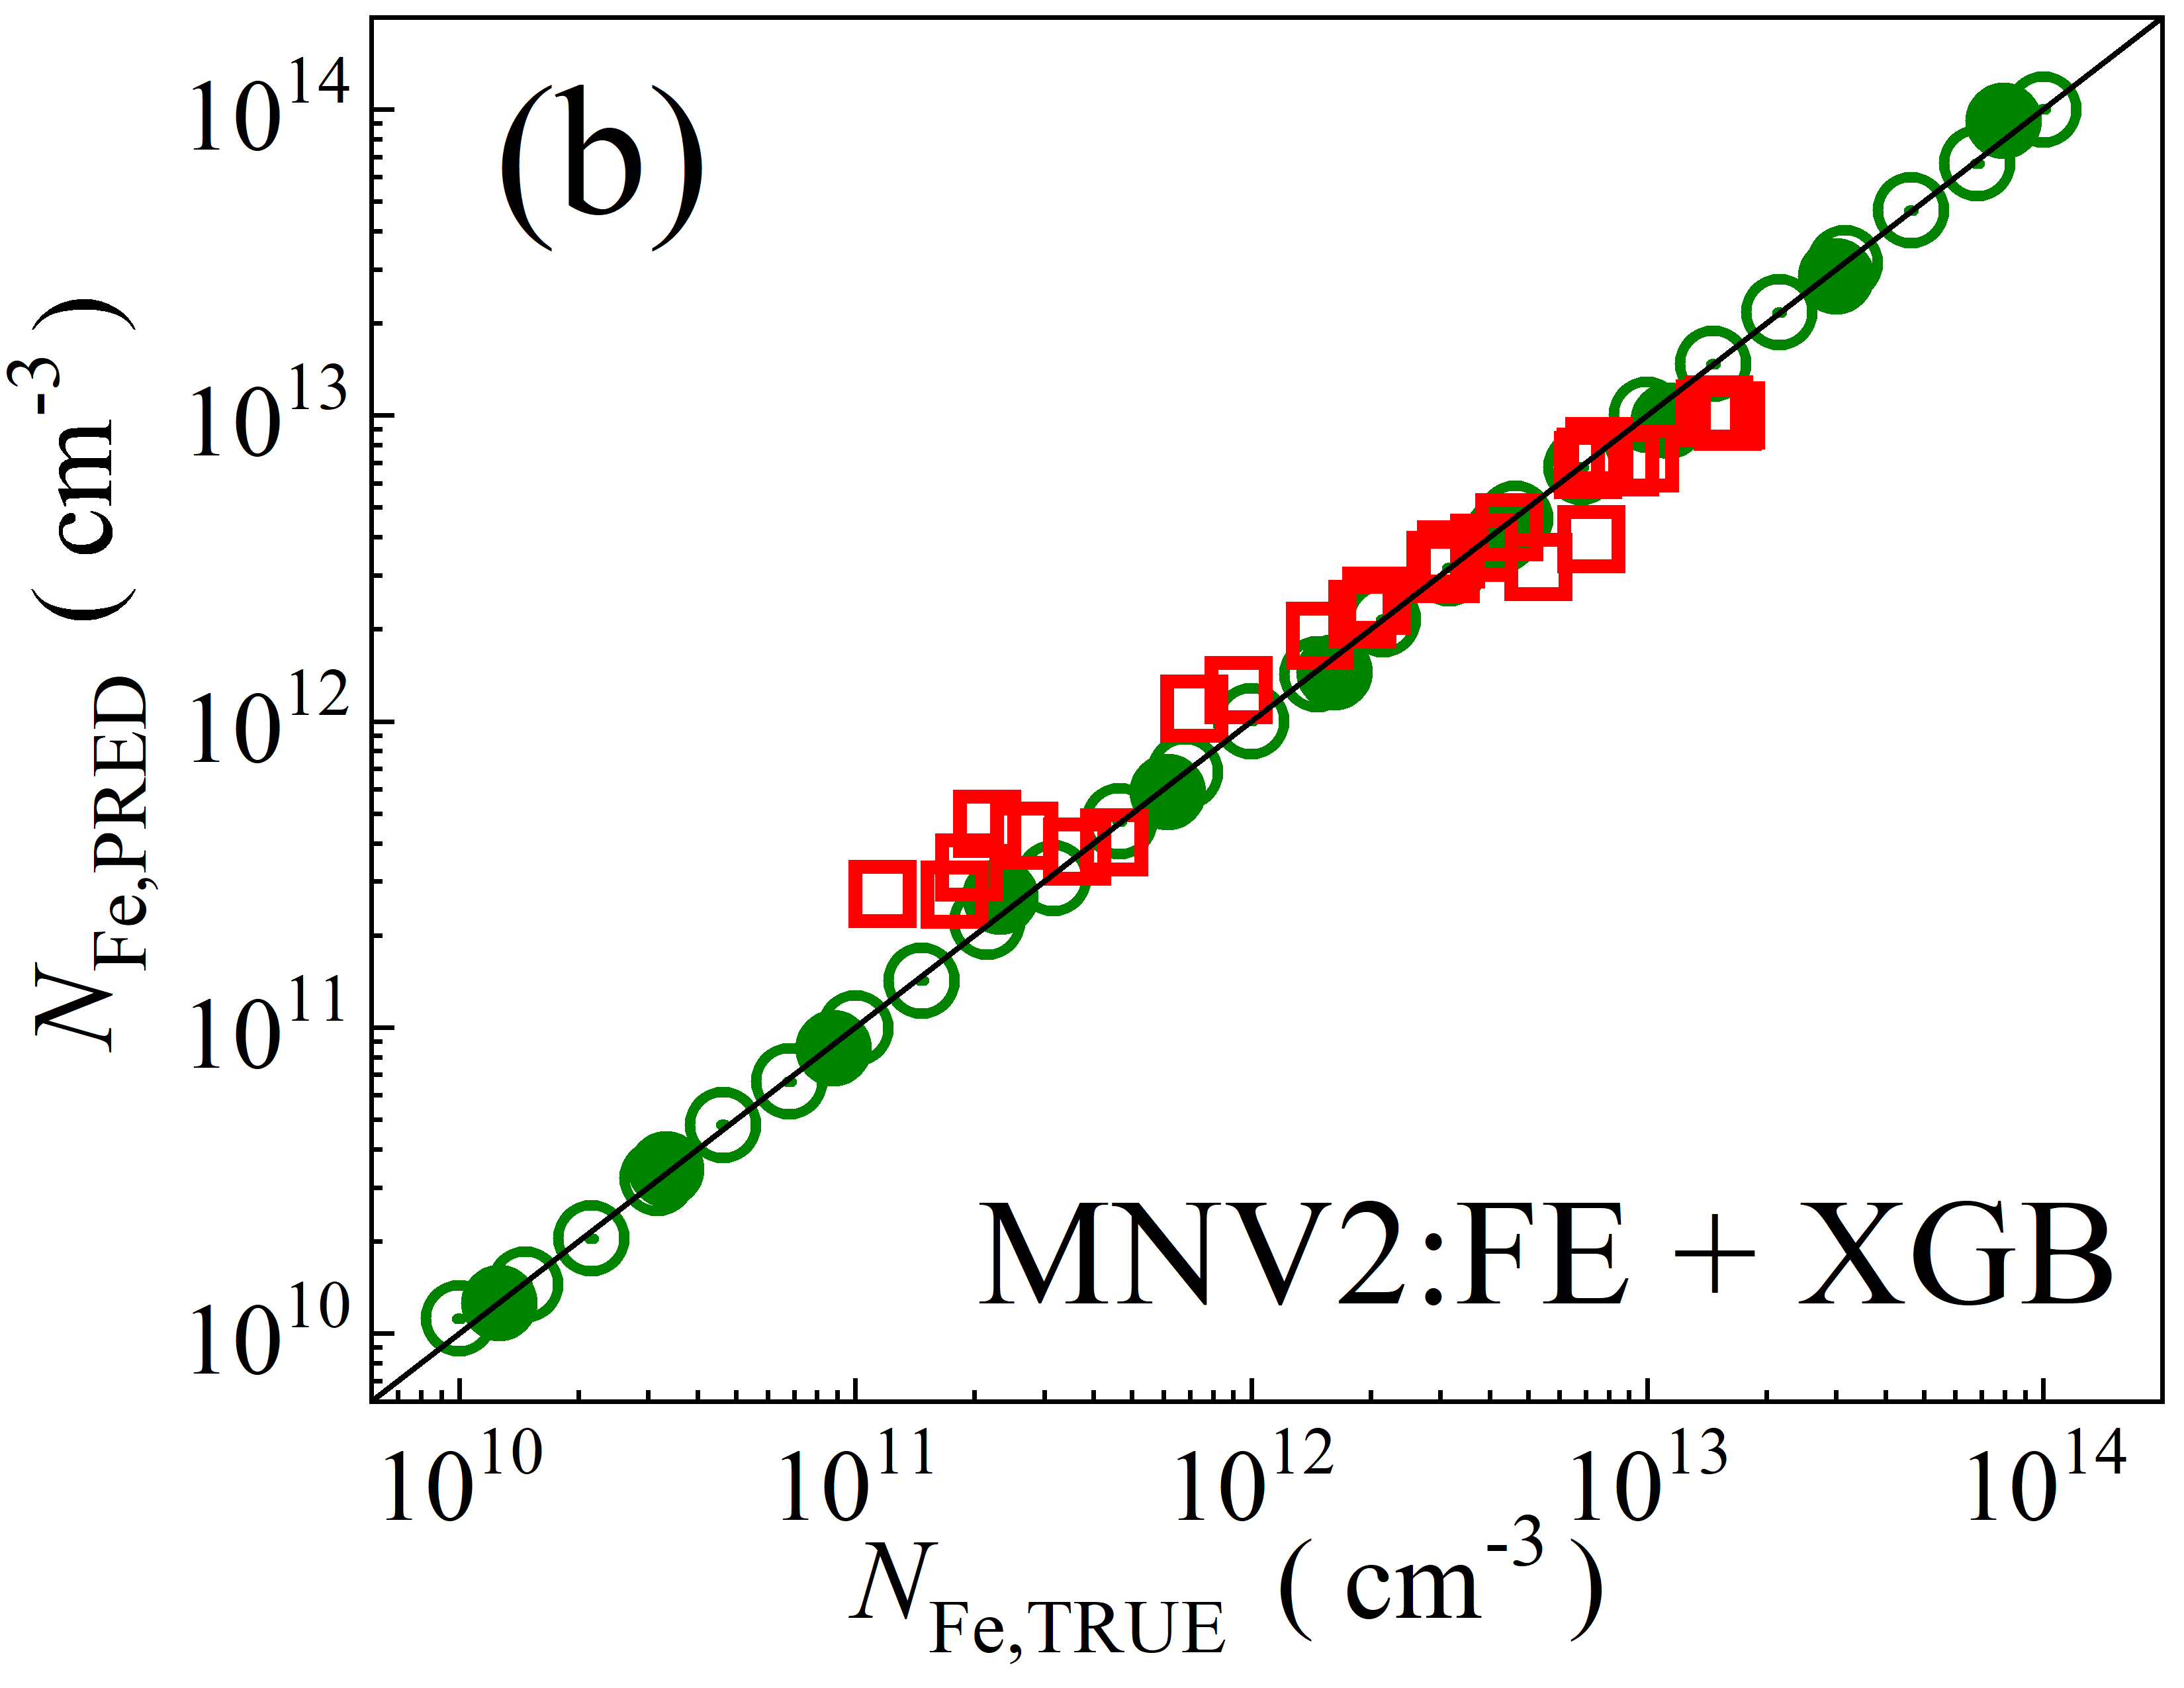
\includegraphics[width=0.24\textwidth]{Fig4b}
%
\includegraphics[width=0.24\textwidth]{Fig4c}
%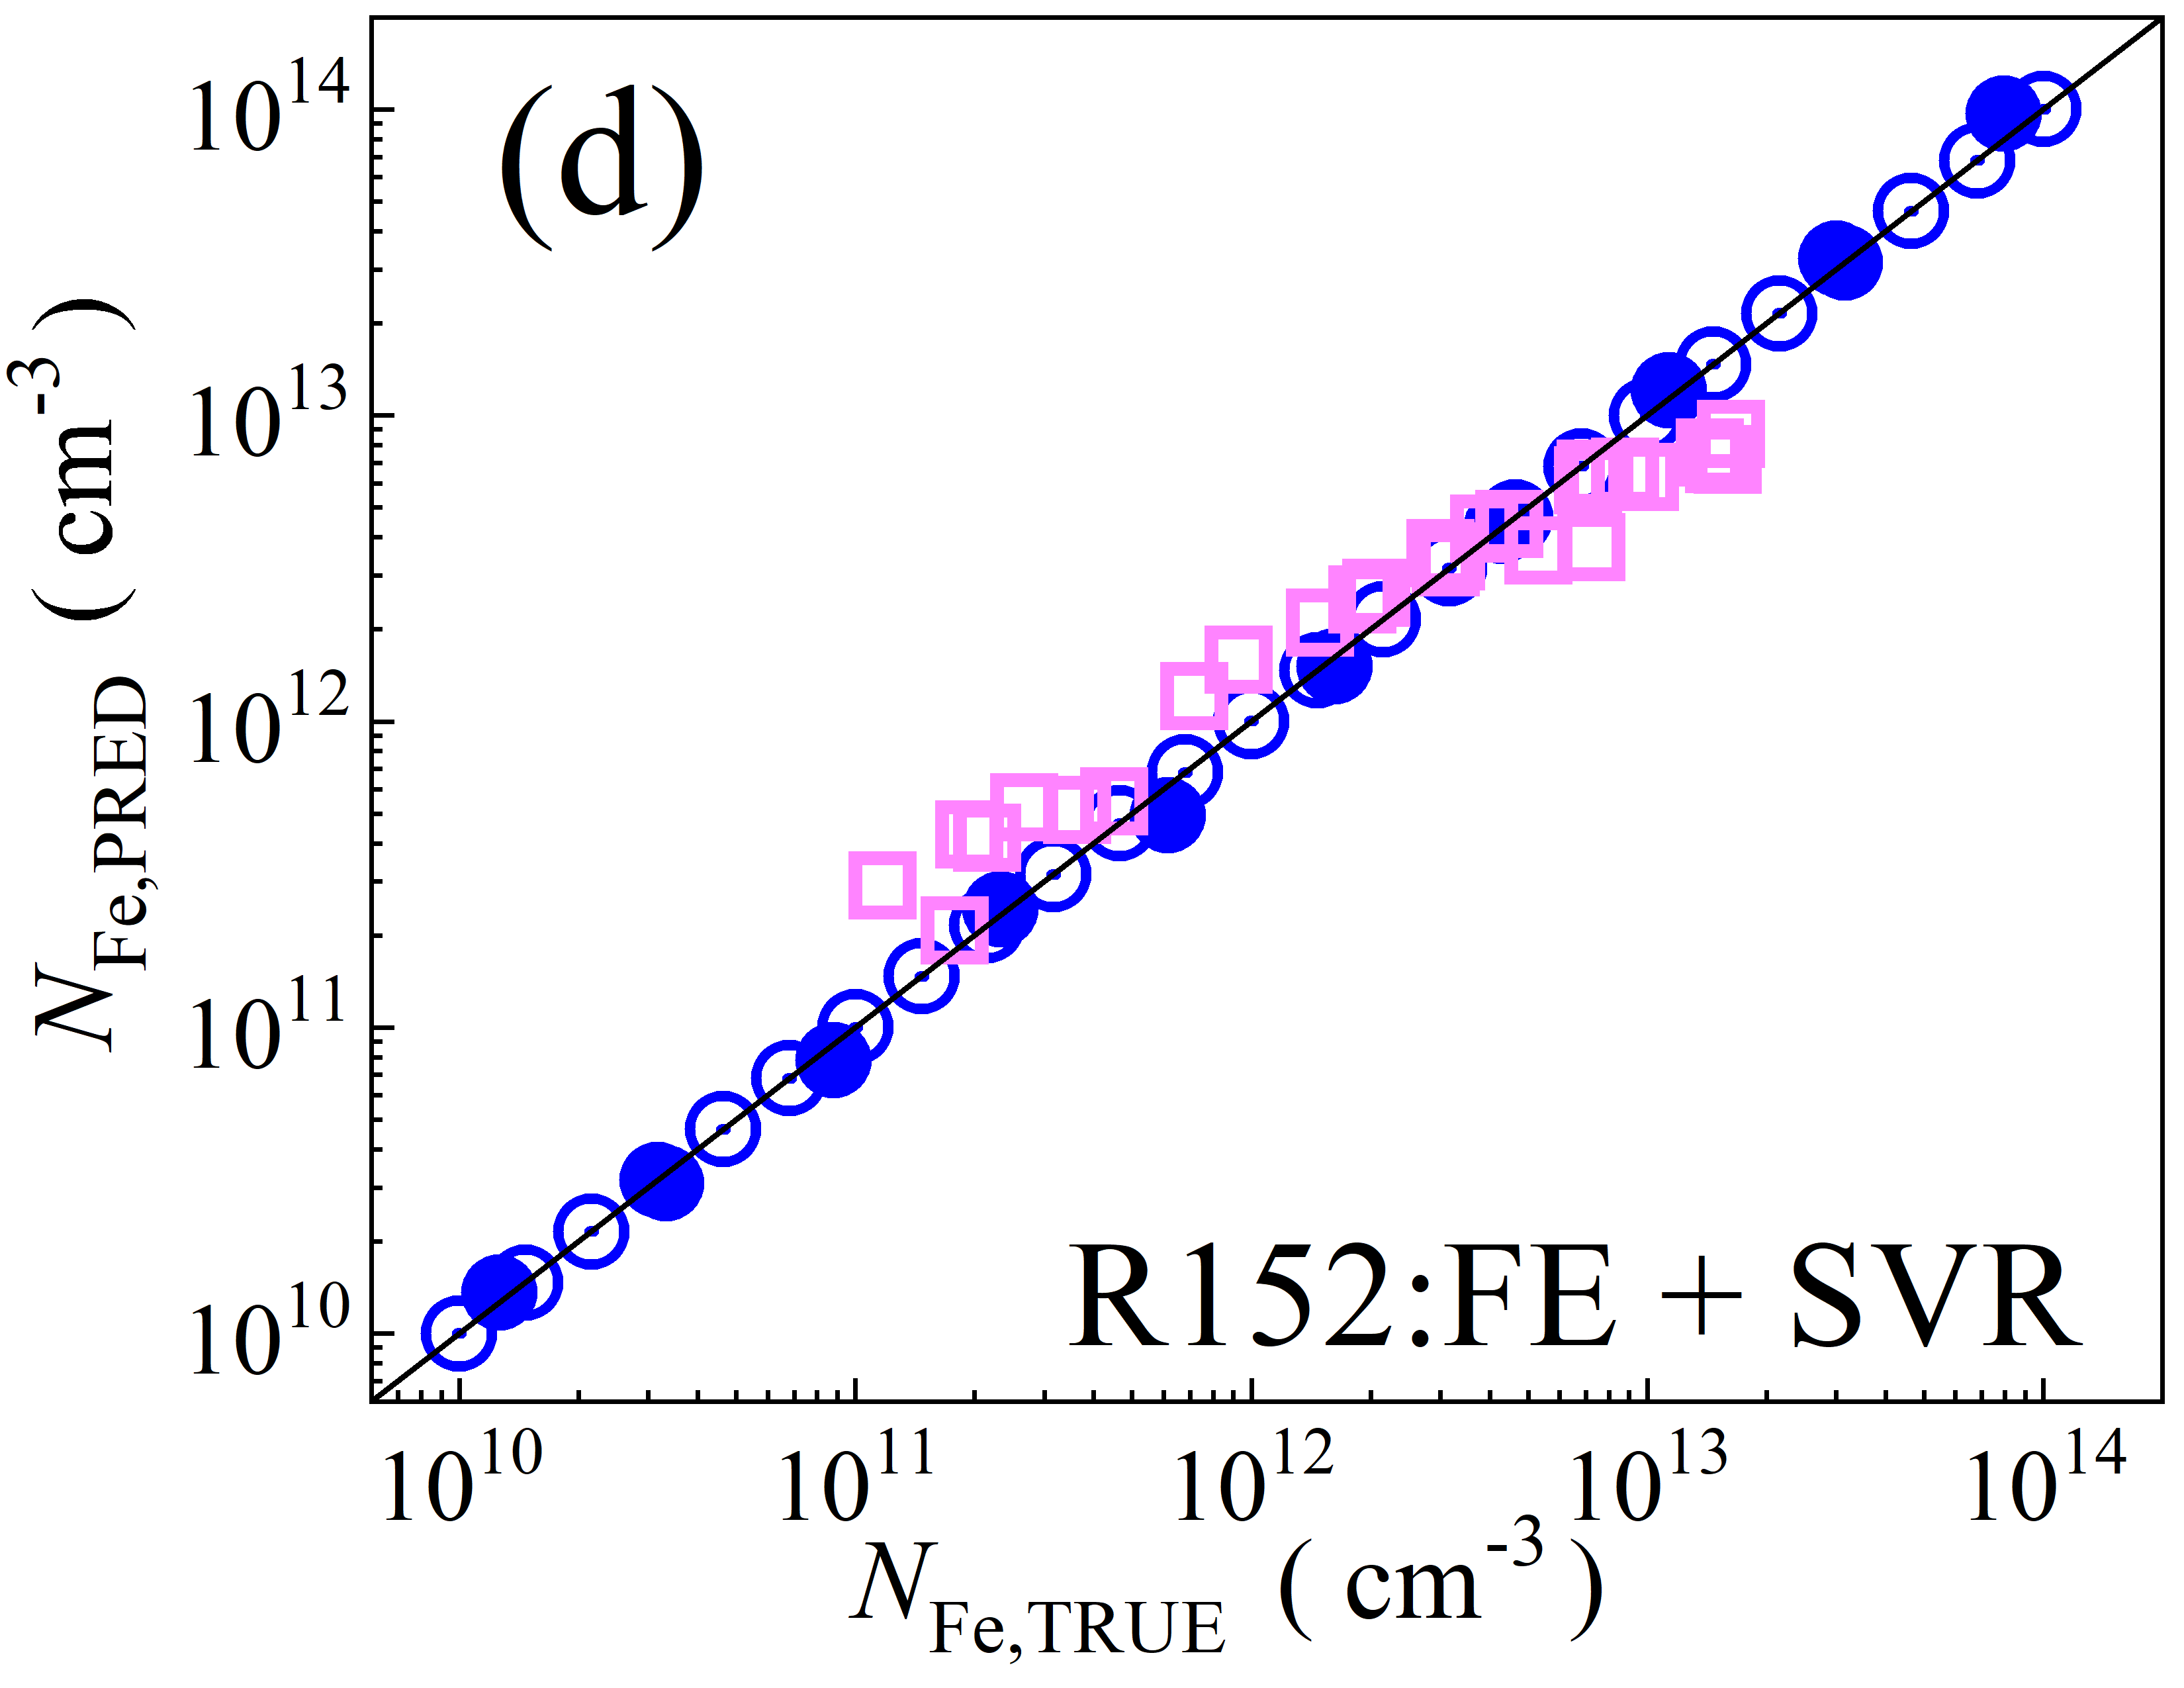
\includegraphics[width=0.24\textwidth]{Fig4d}
%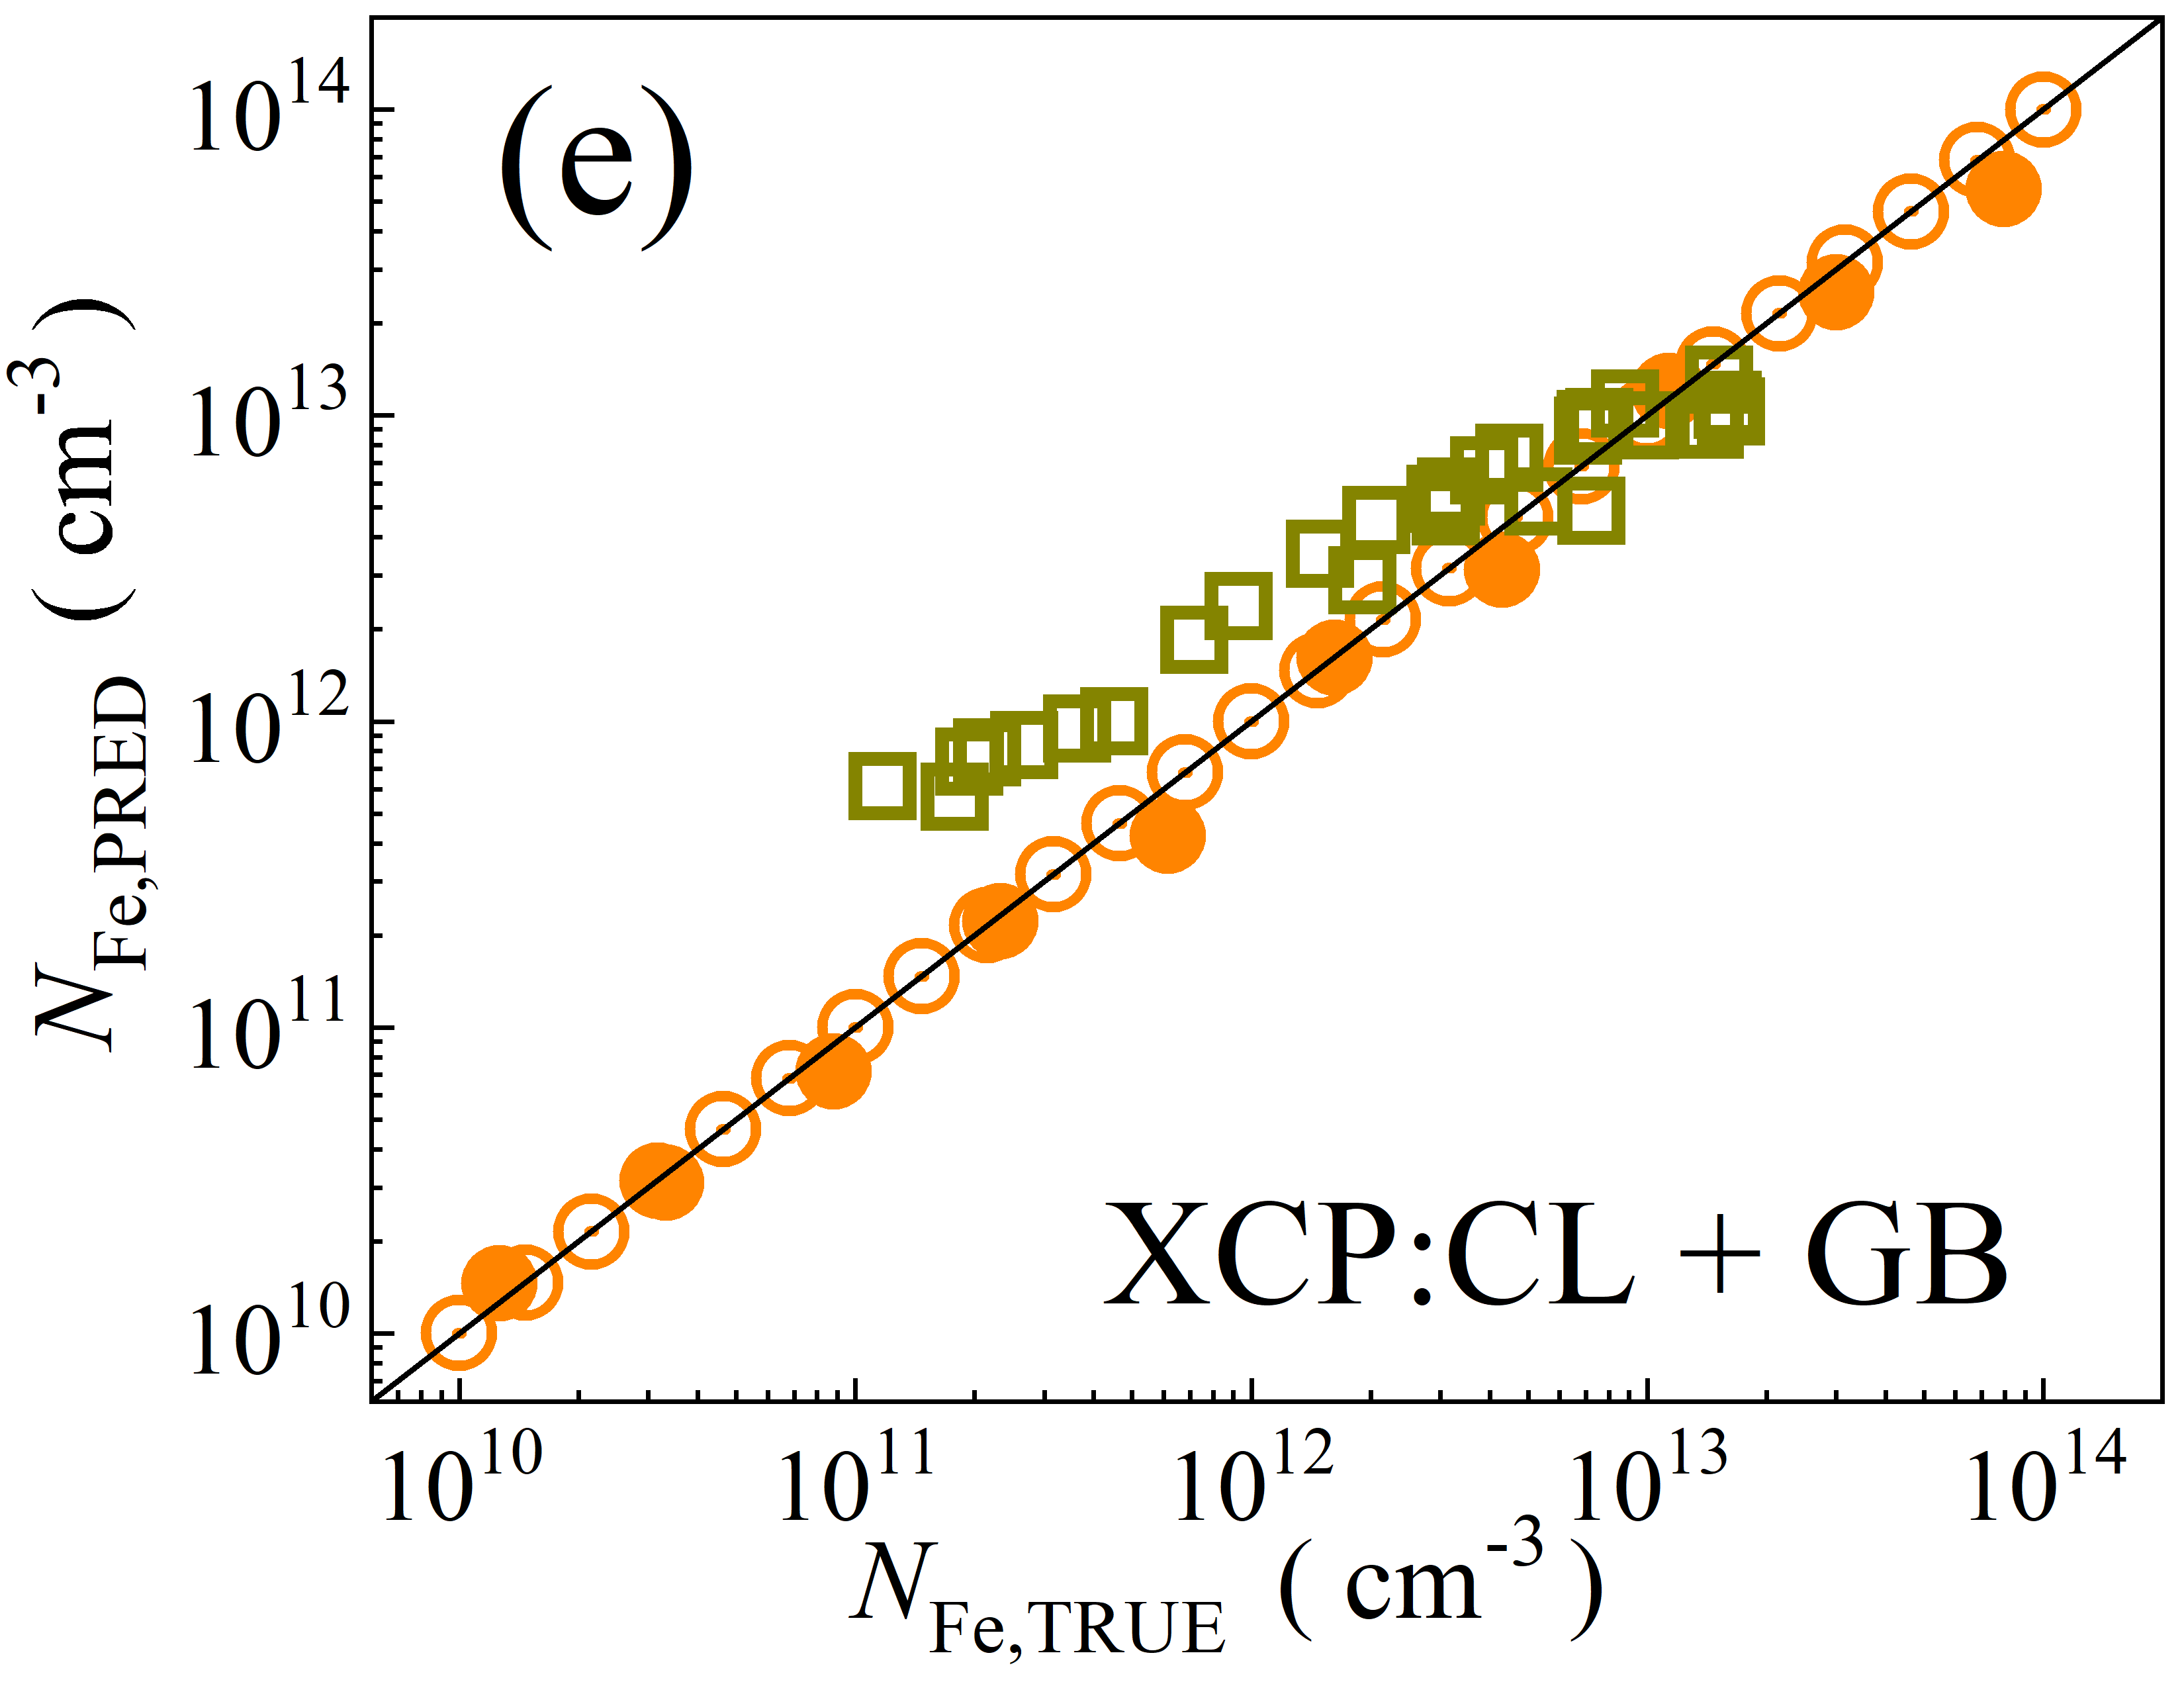
\includegraphics[width=0.24\textwidth]{Fig4e}
%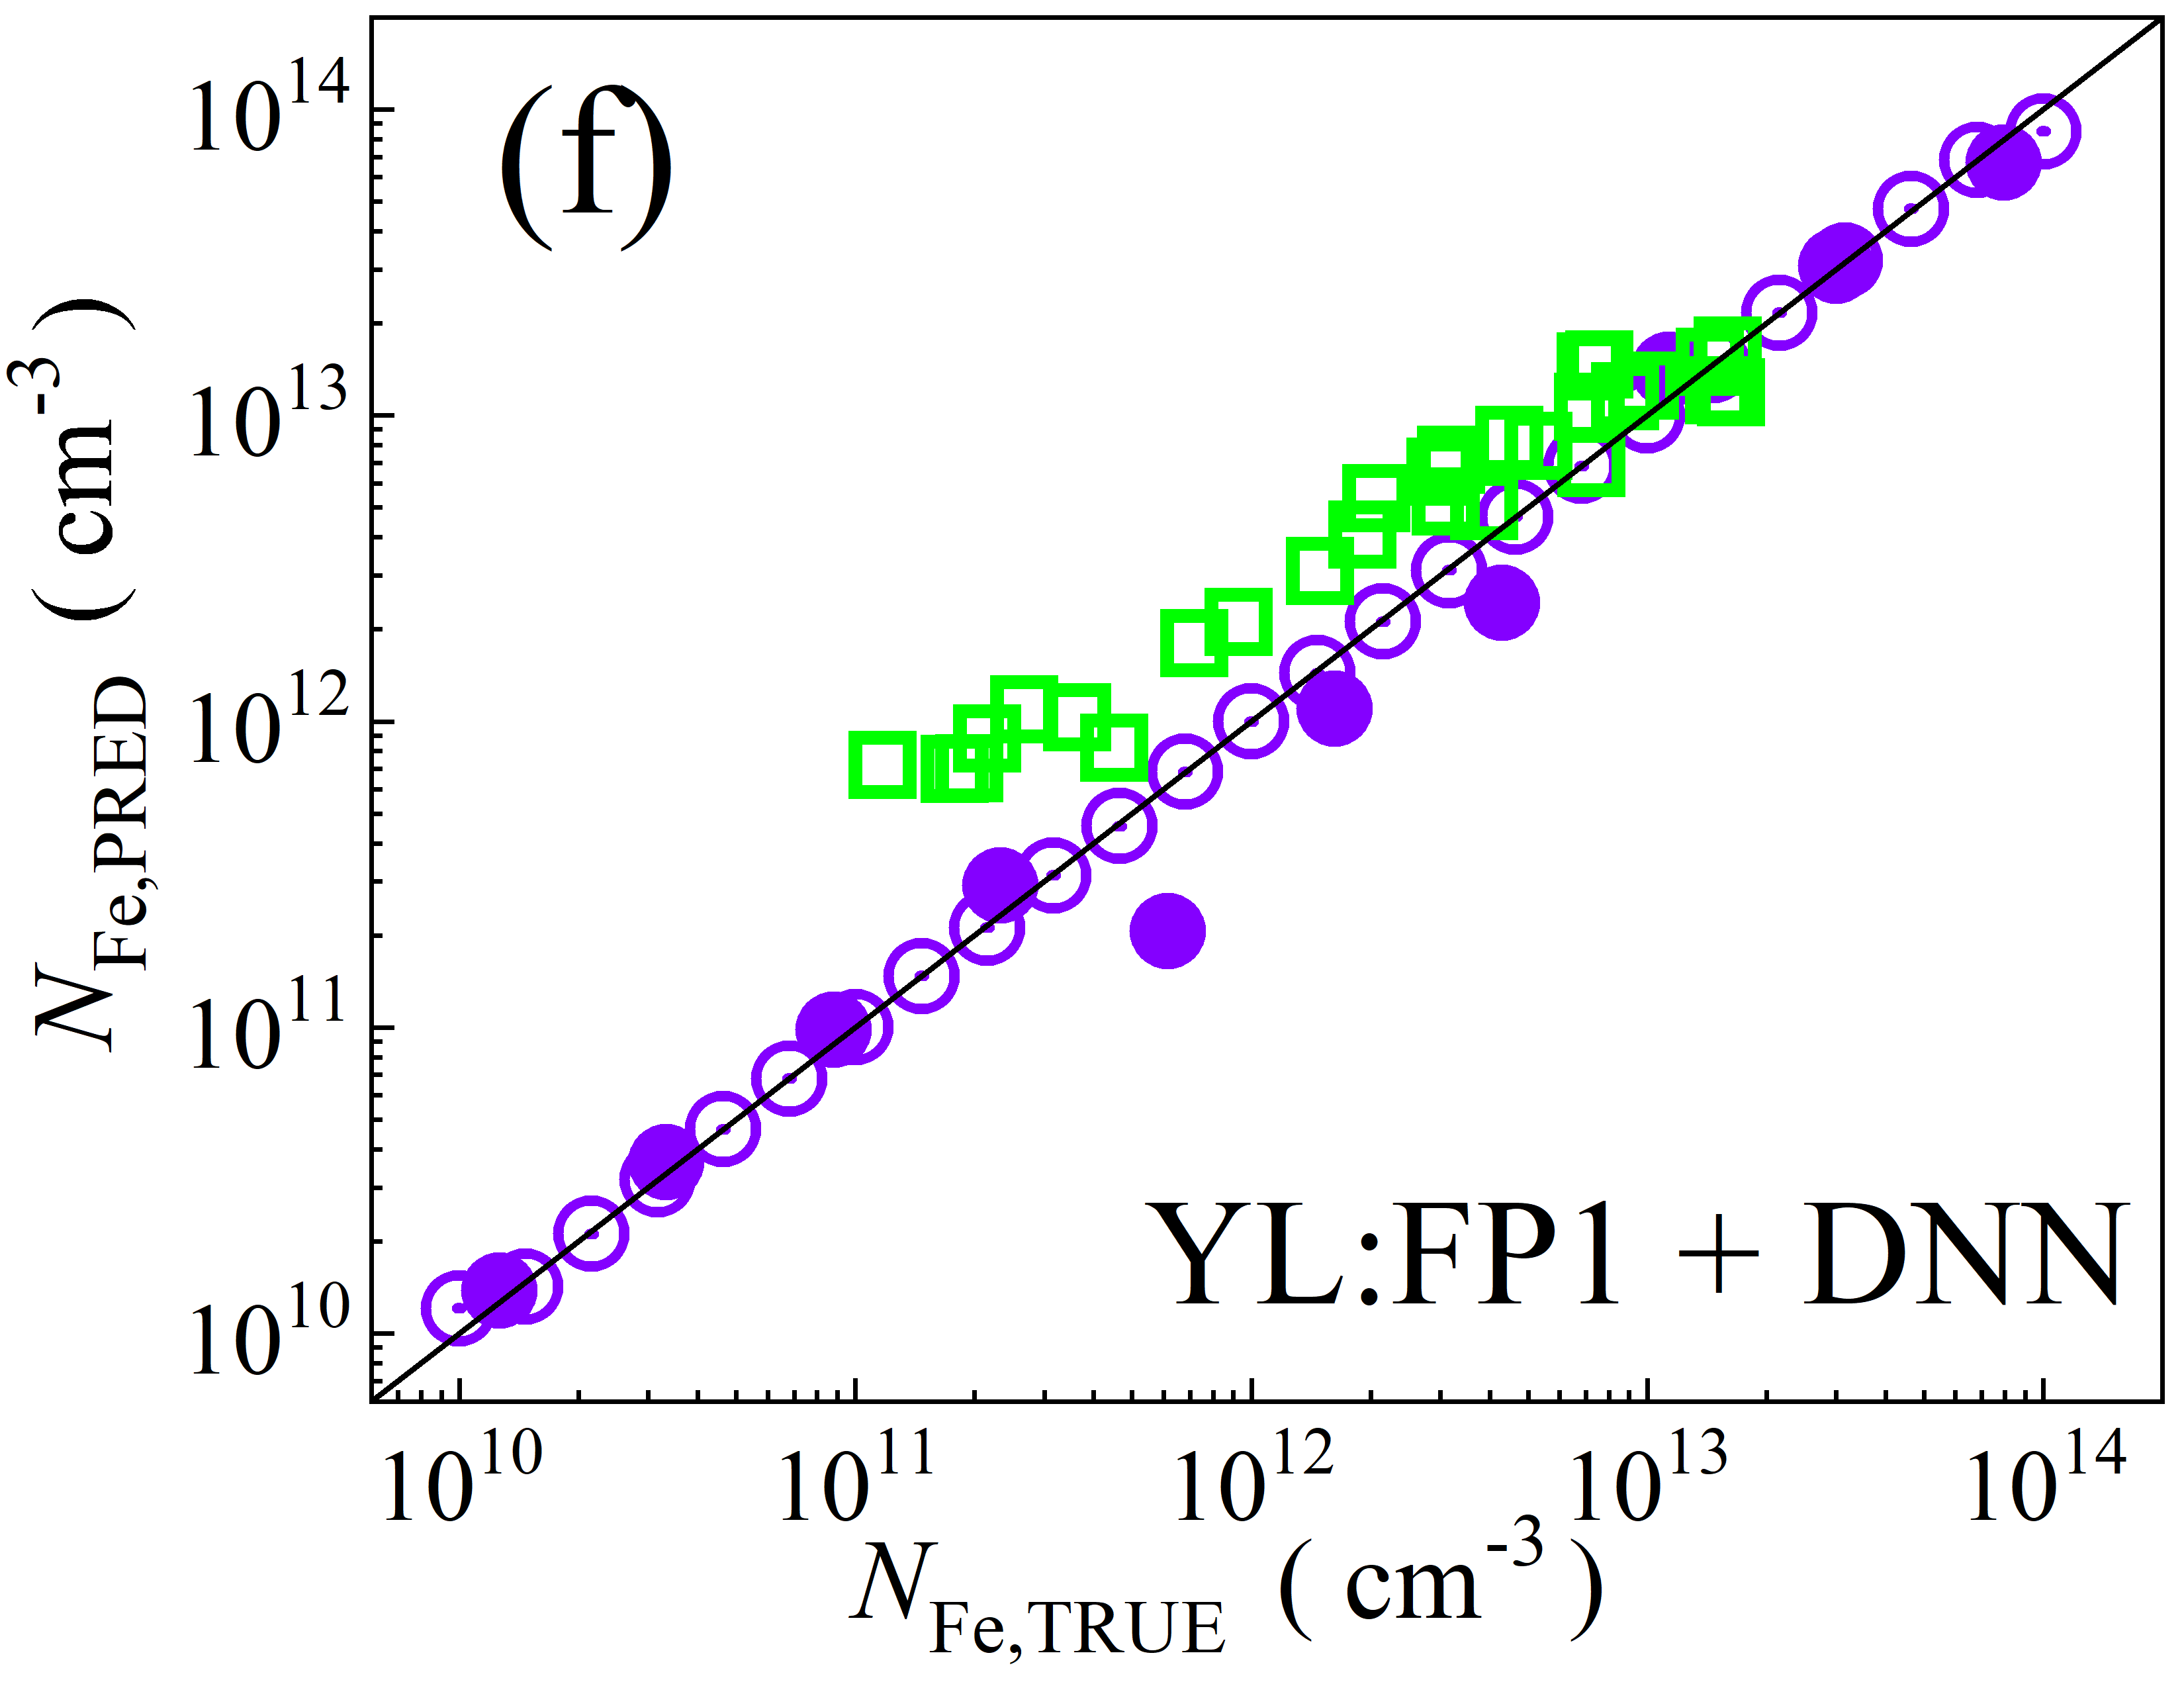
\includegraphics[width=0.24\textwidth]{Fig4f}
%\caption{
%The workflow of the ML pipeline
%}\label{Fig4}
%\end{figure*}

\begin{figure*}
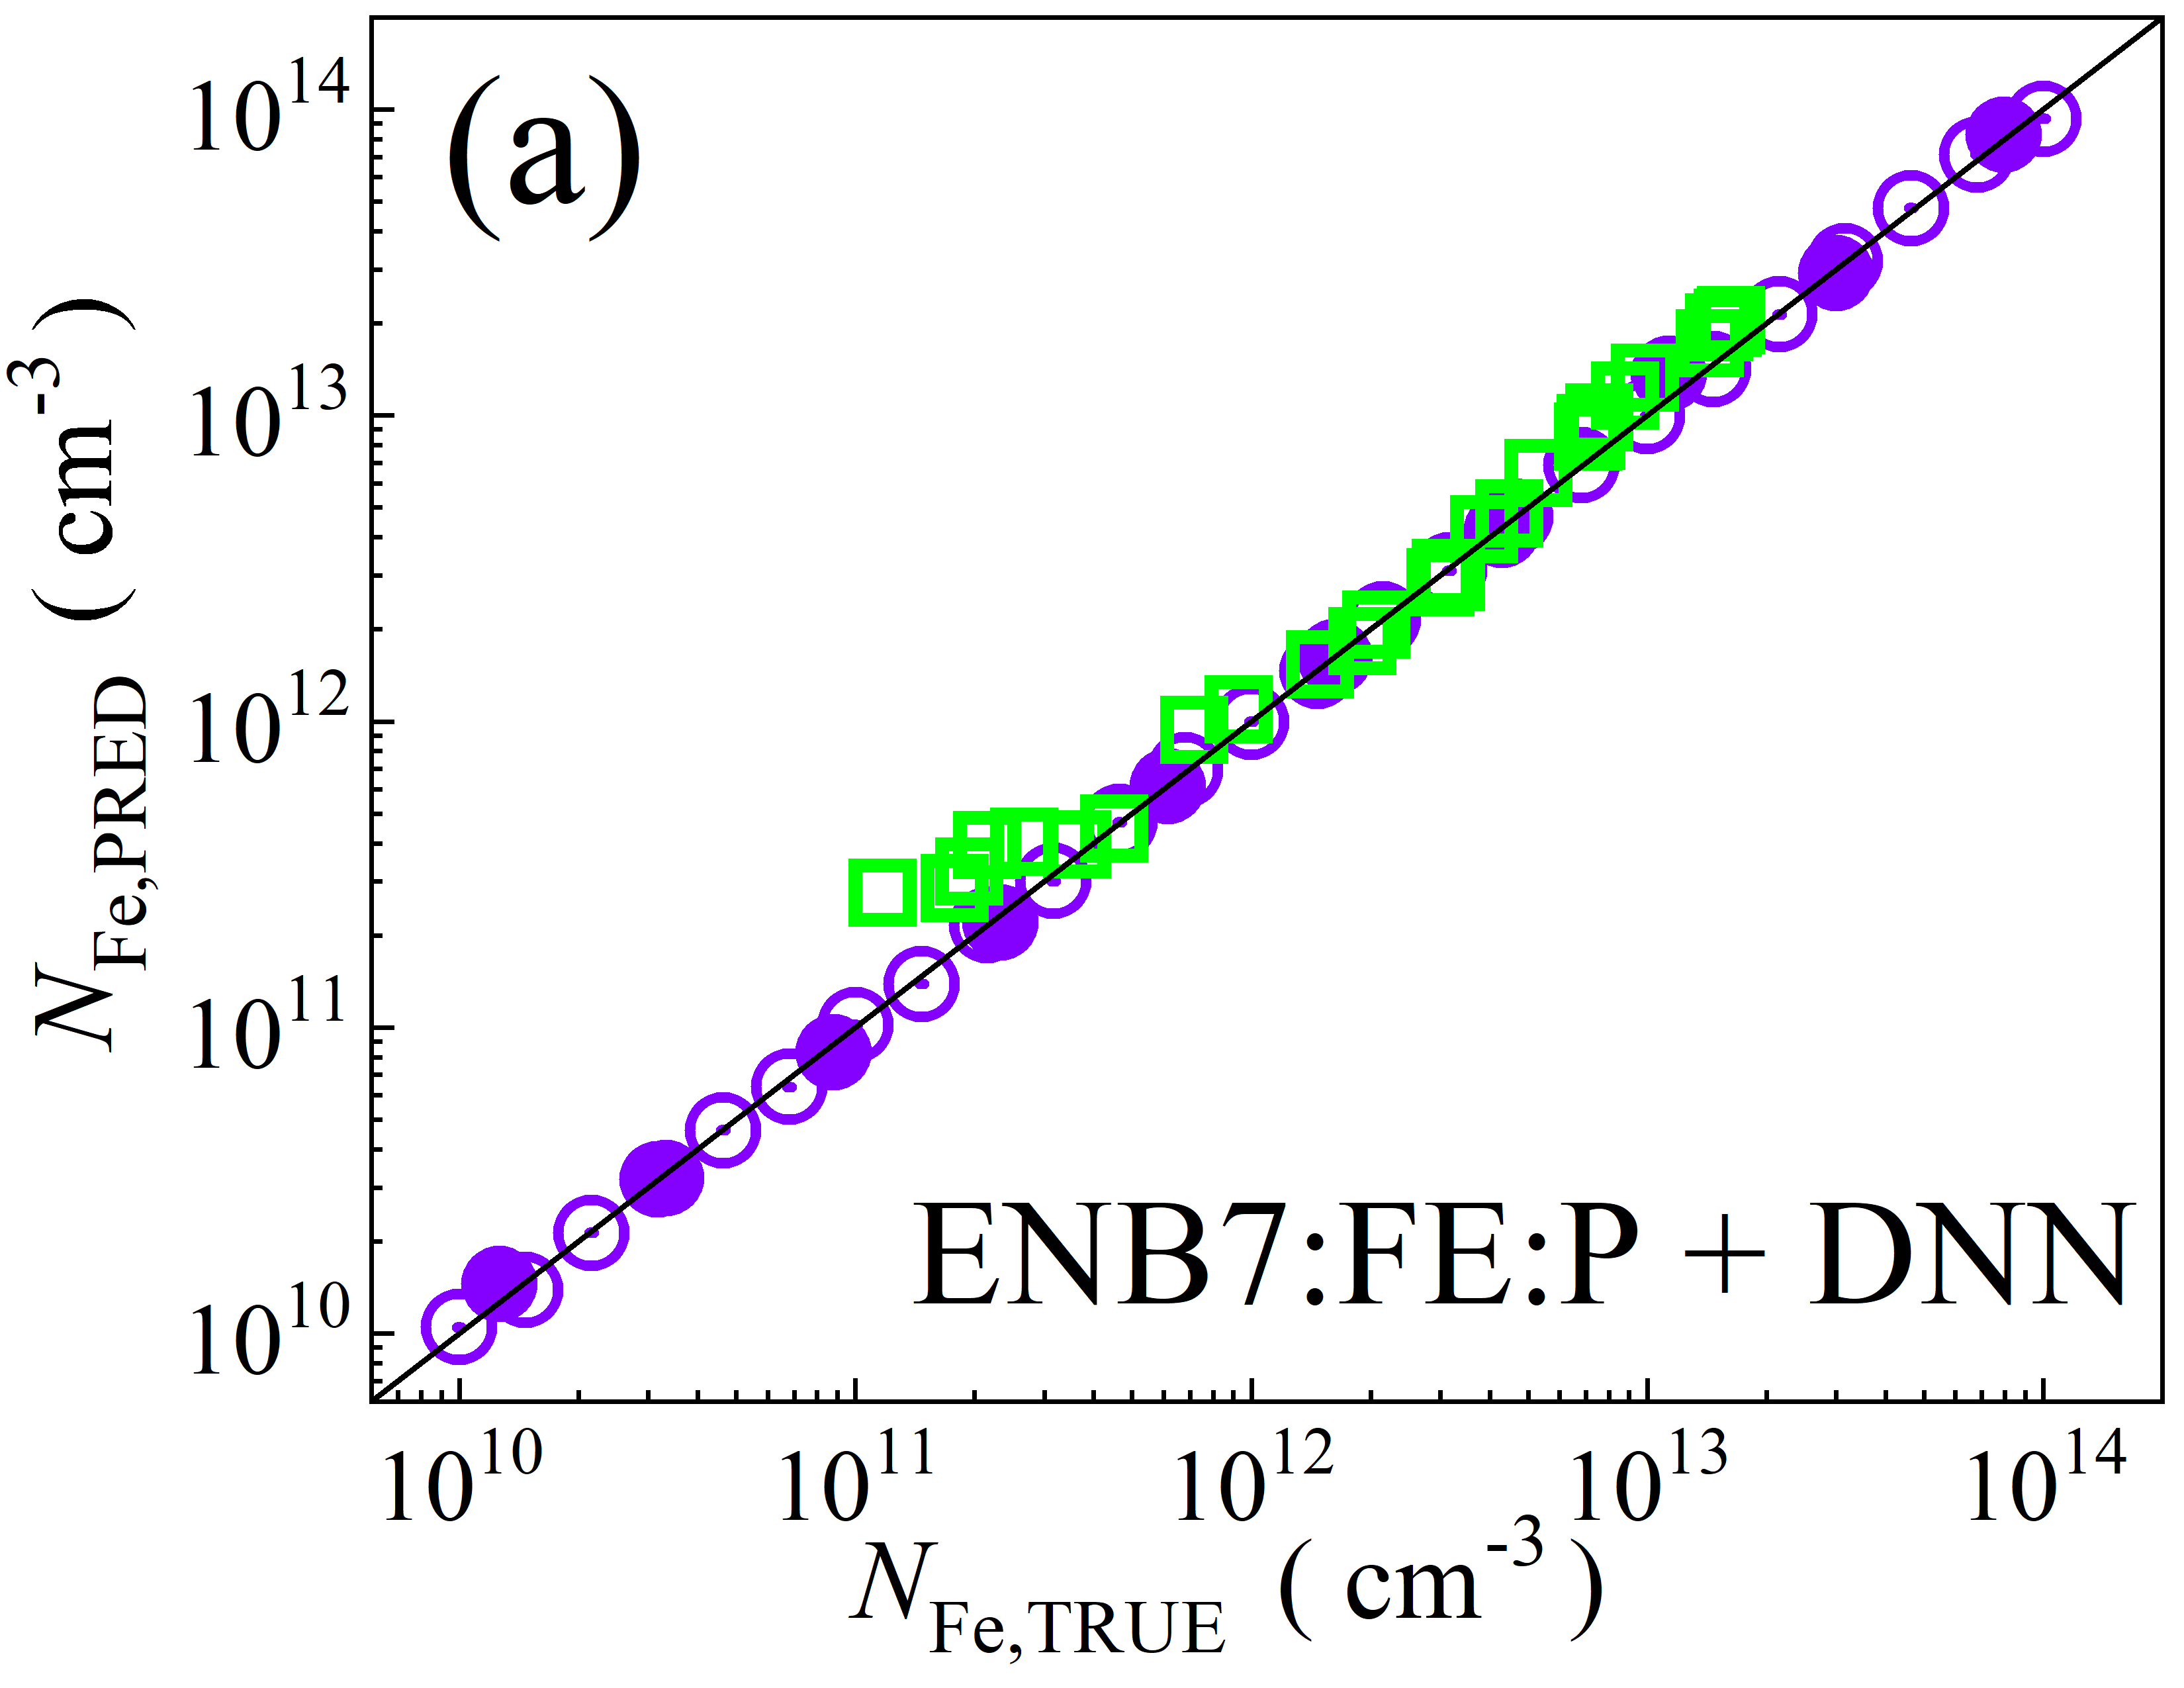
\includegraphics[width=0.33\textwidth]{Fig4a}
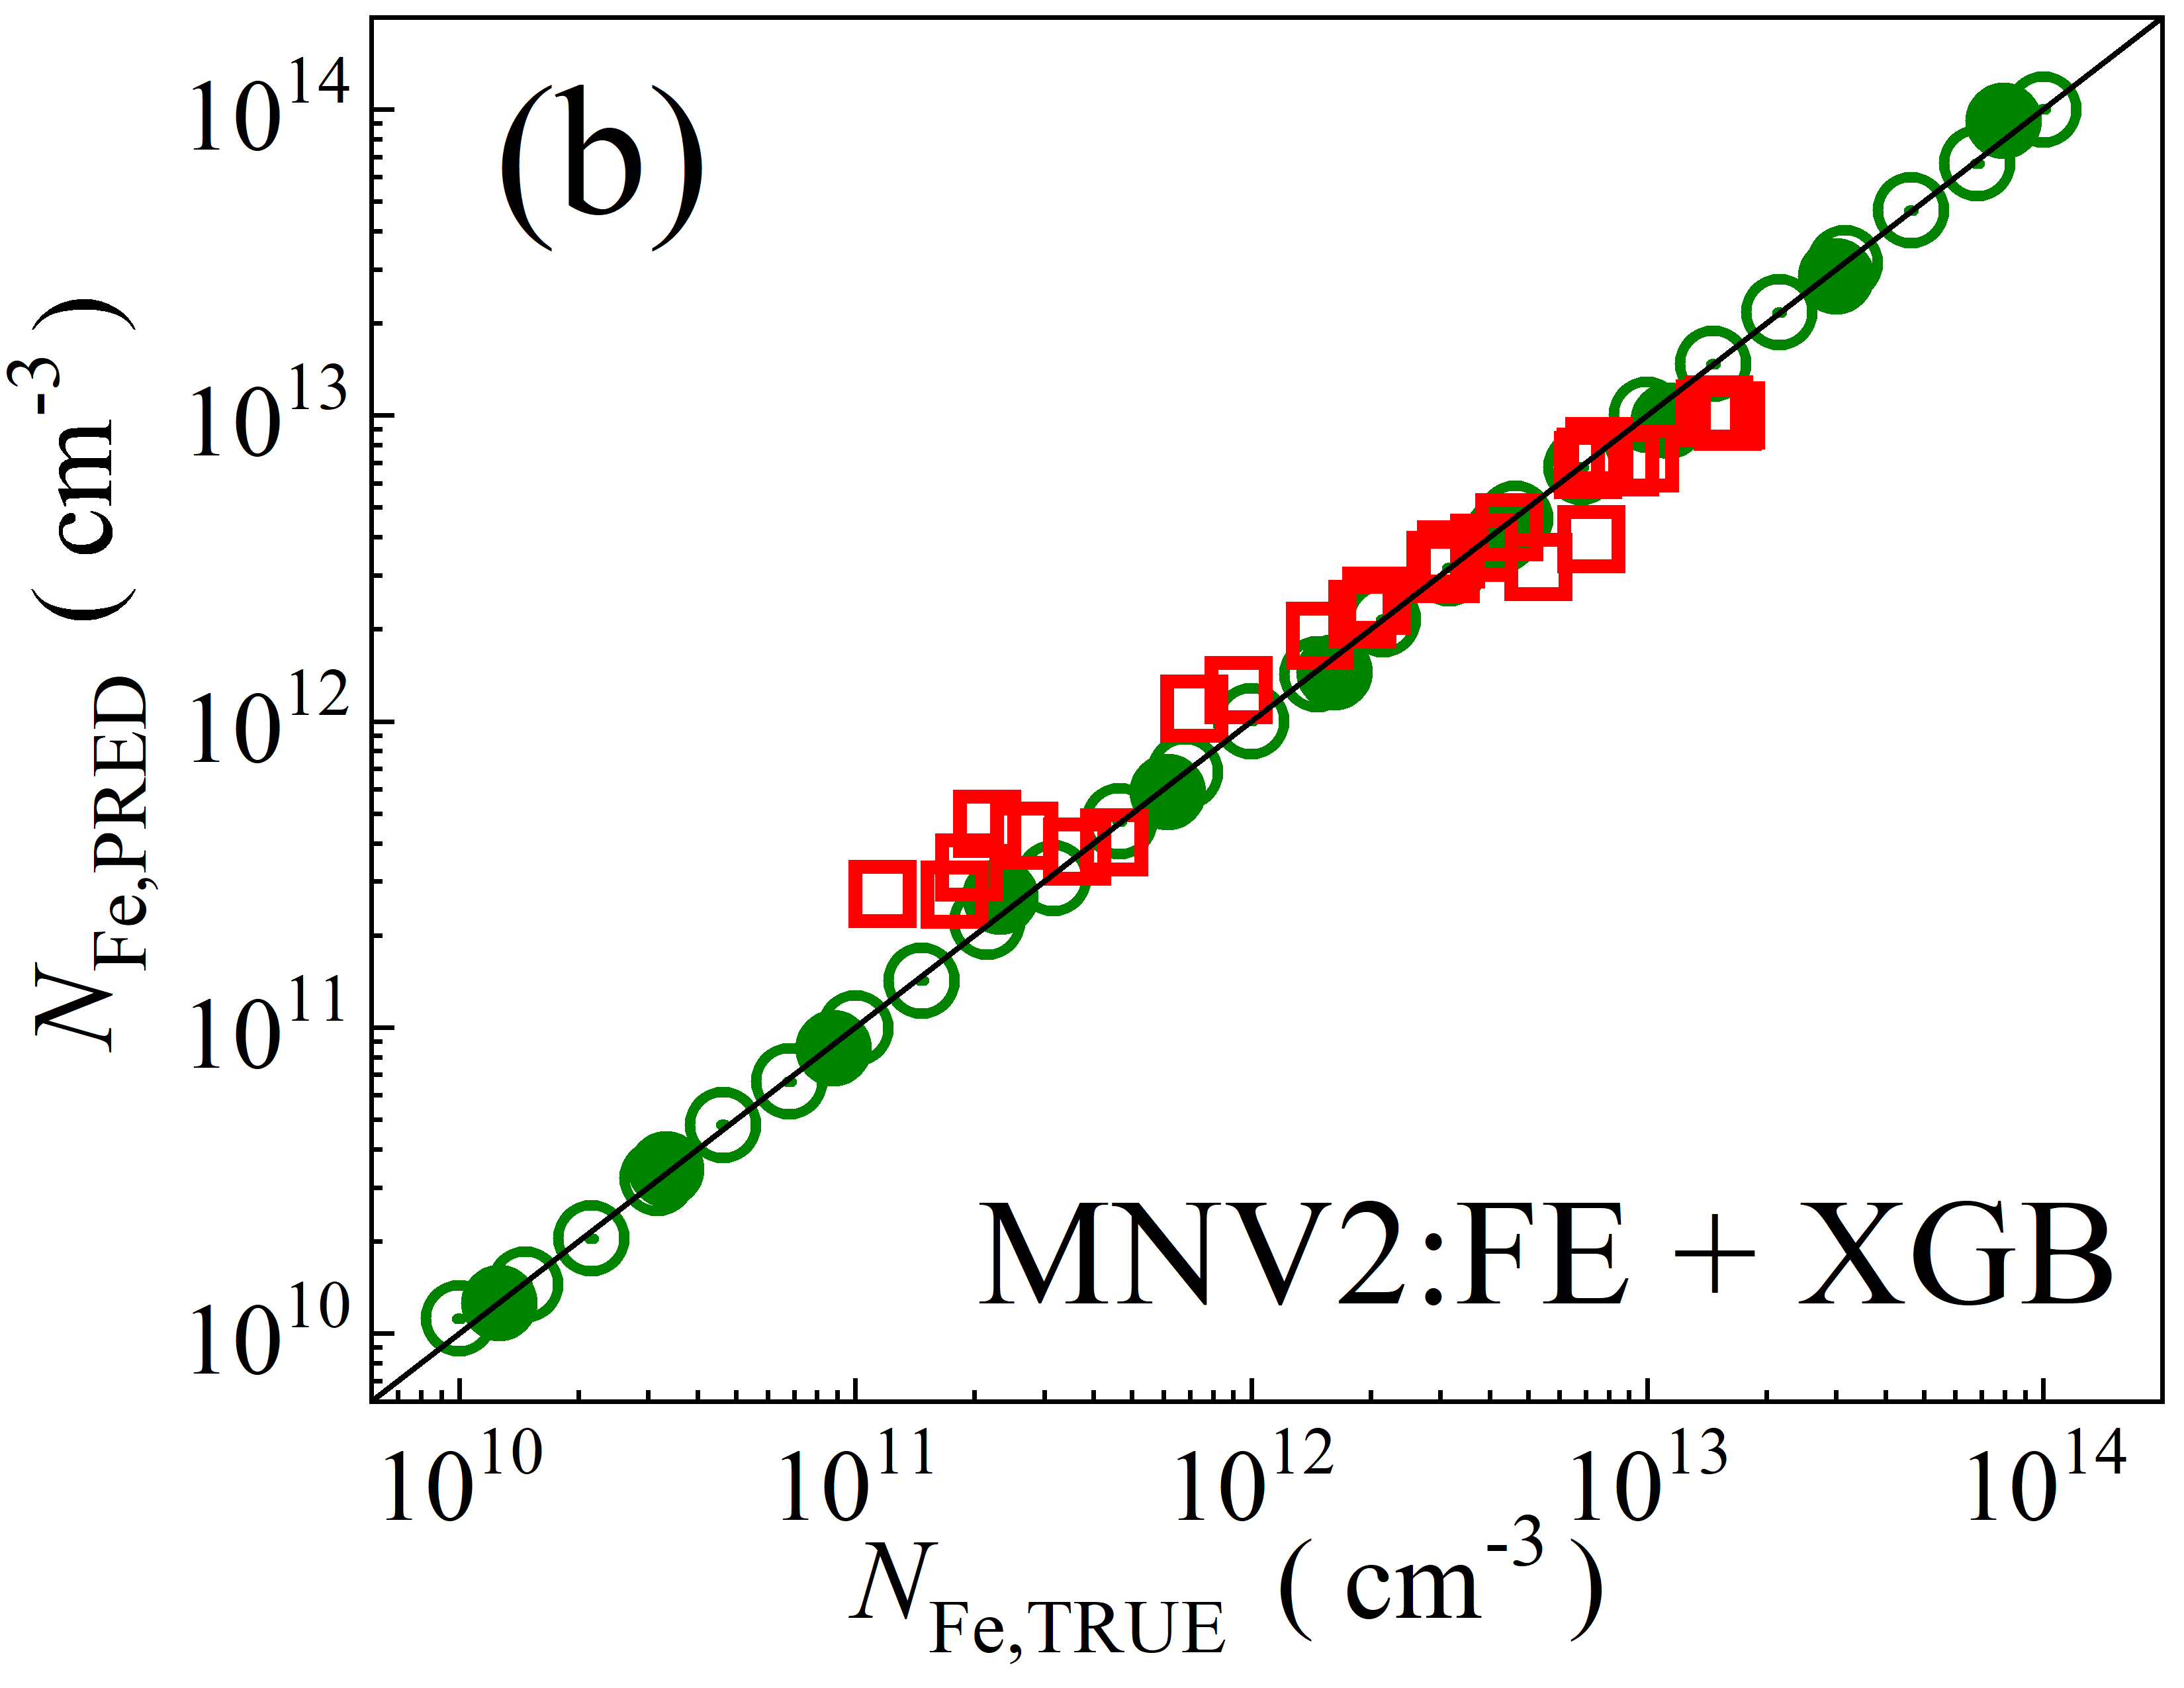
\includegraphics[width=0.33\textwidth]{Fig4b}

\includegraphics[width=0.33\textwidth]{Fig4c}
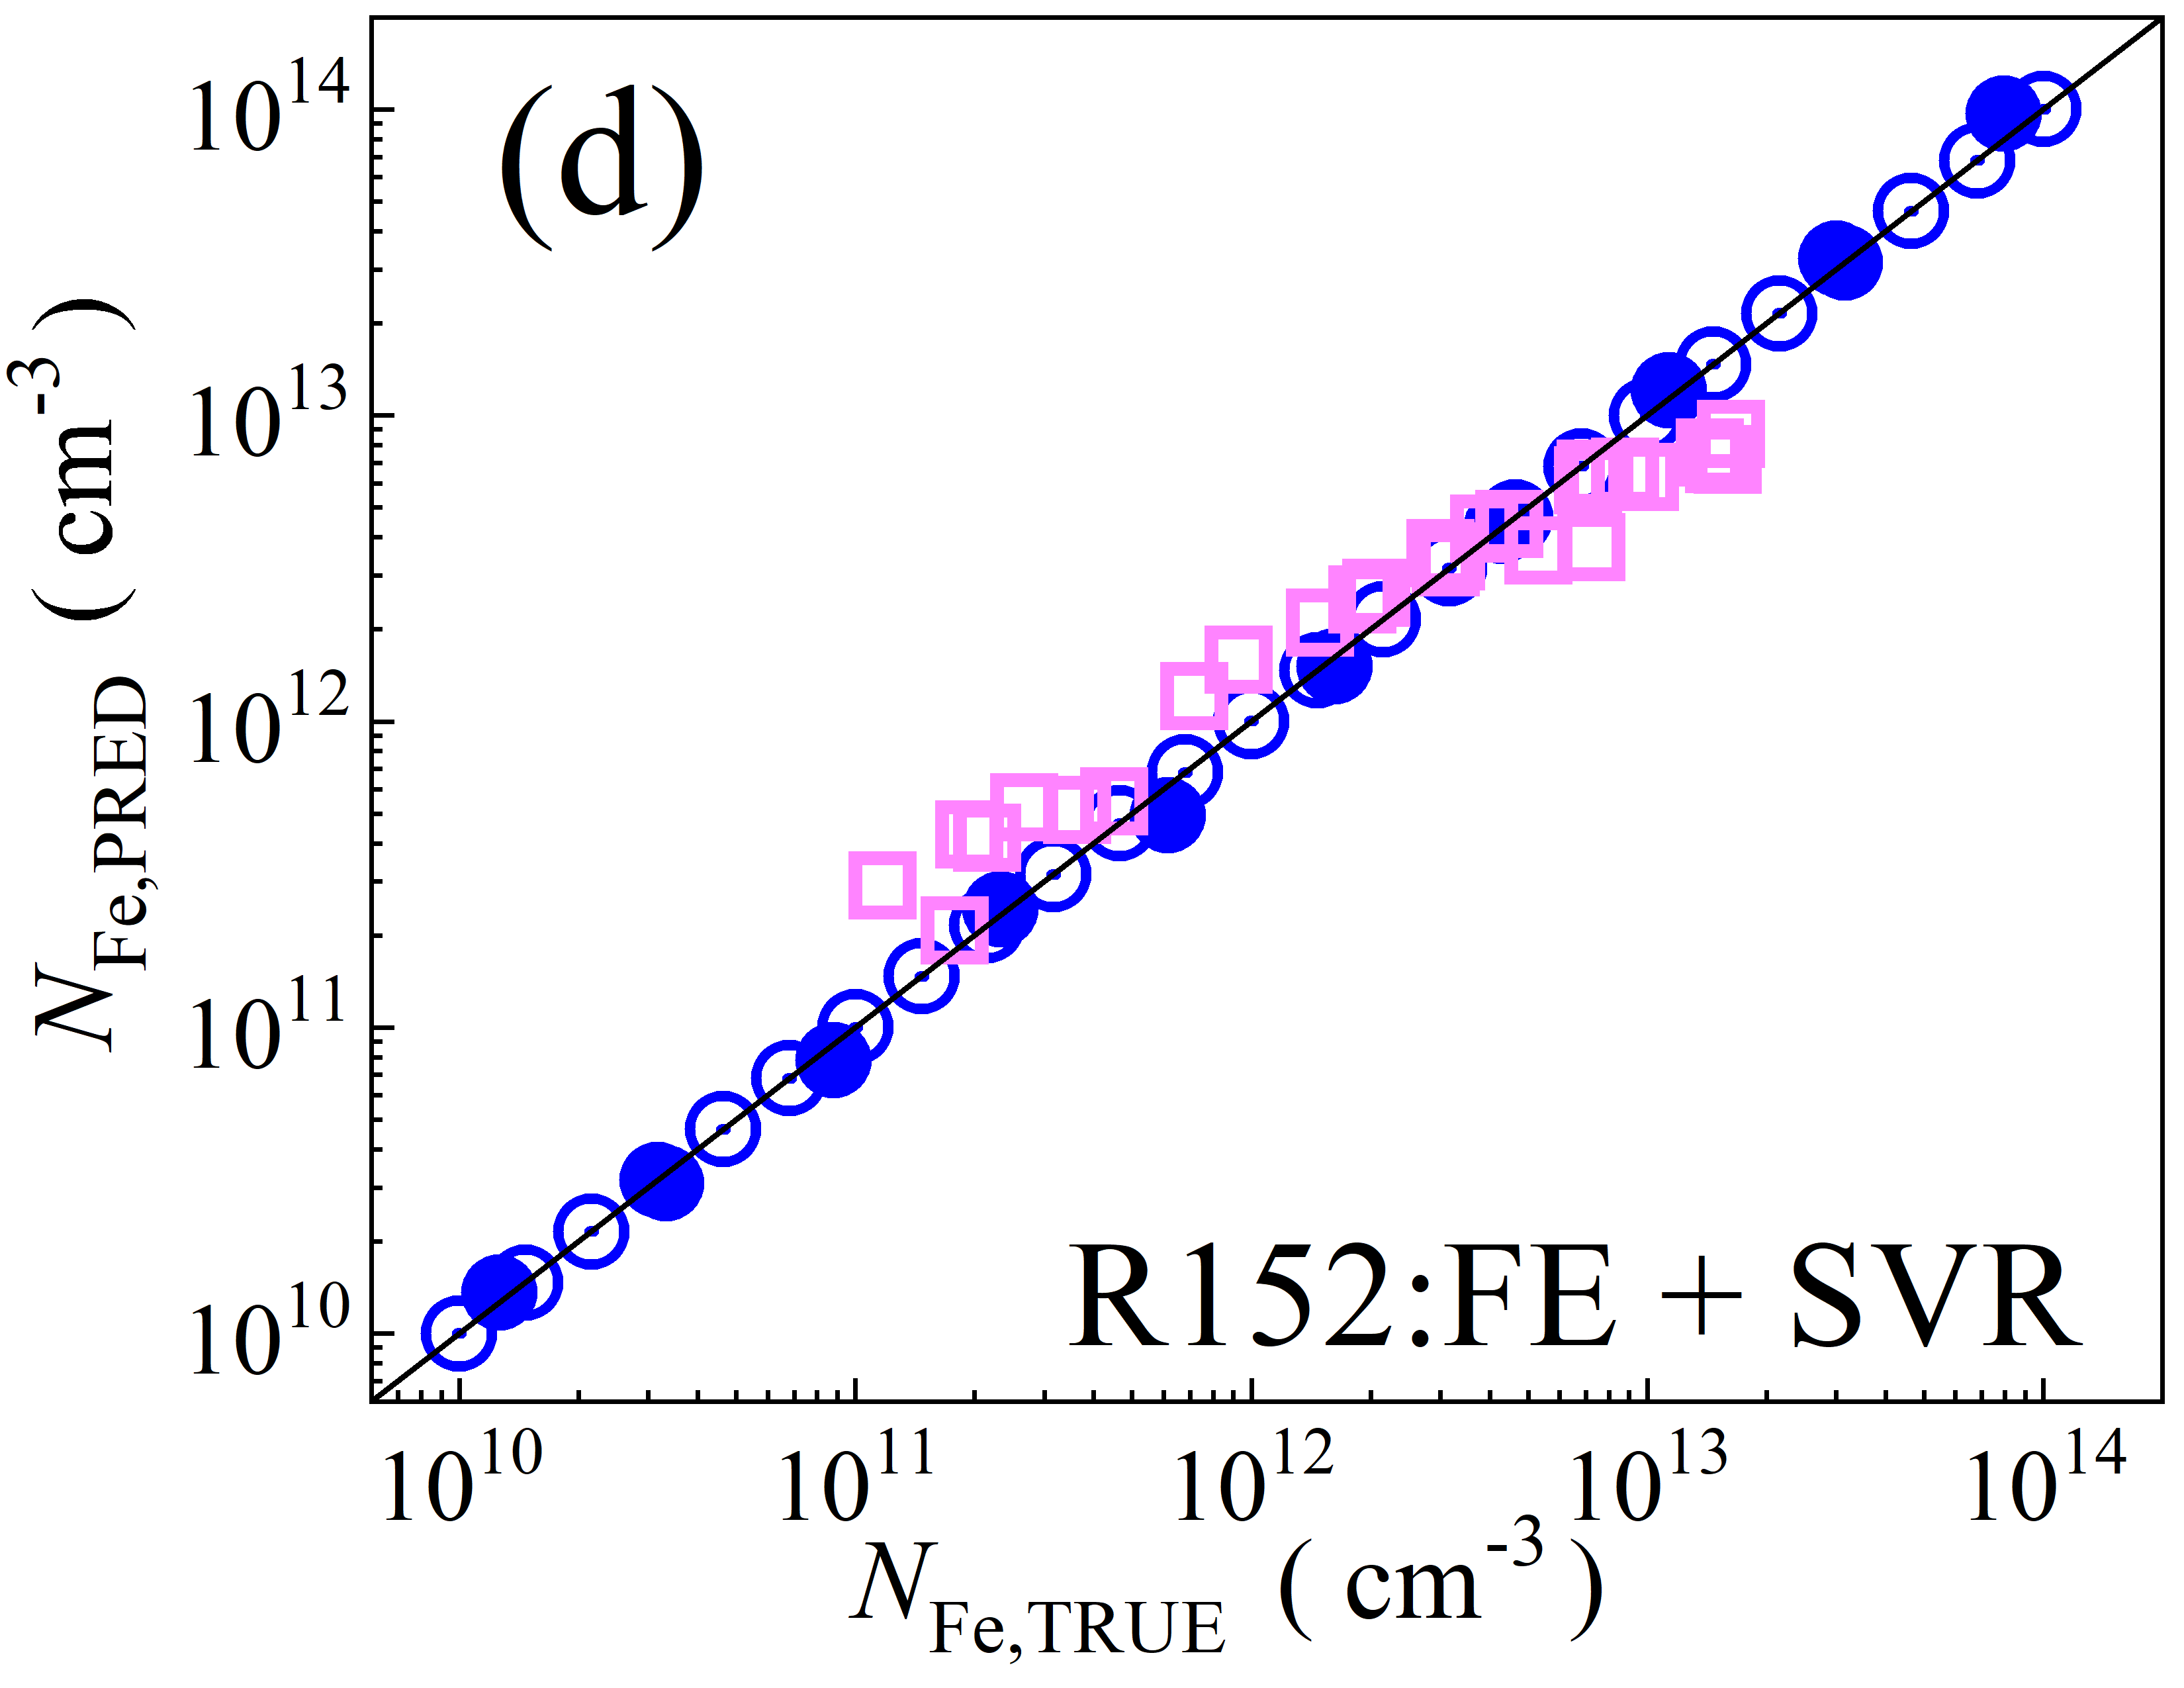
\includegraphics[width=0.33\textwidth]{Fig4d}
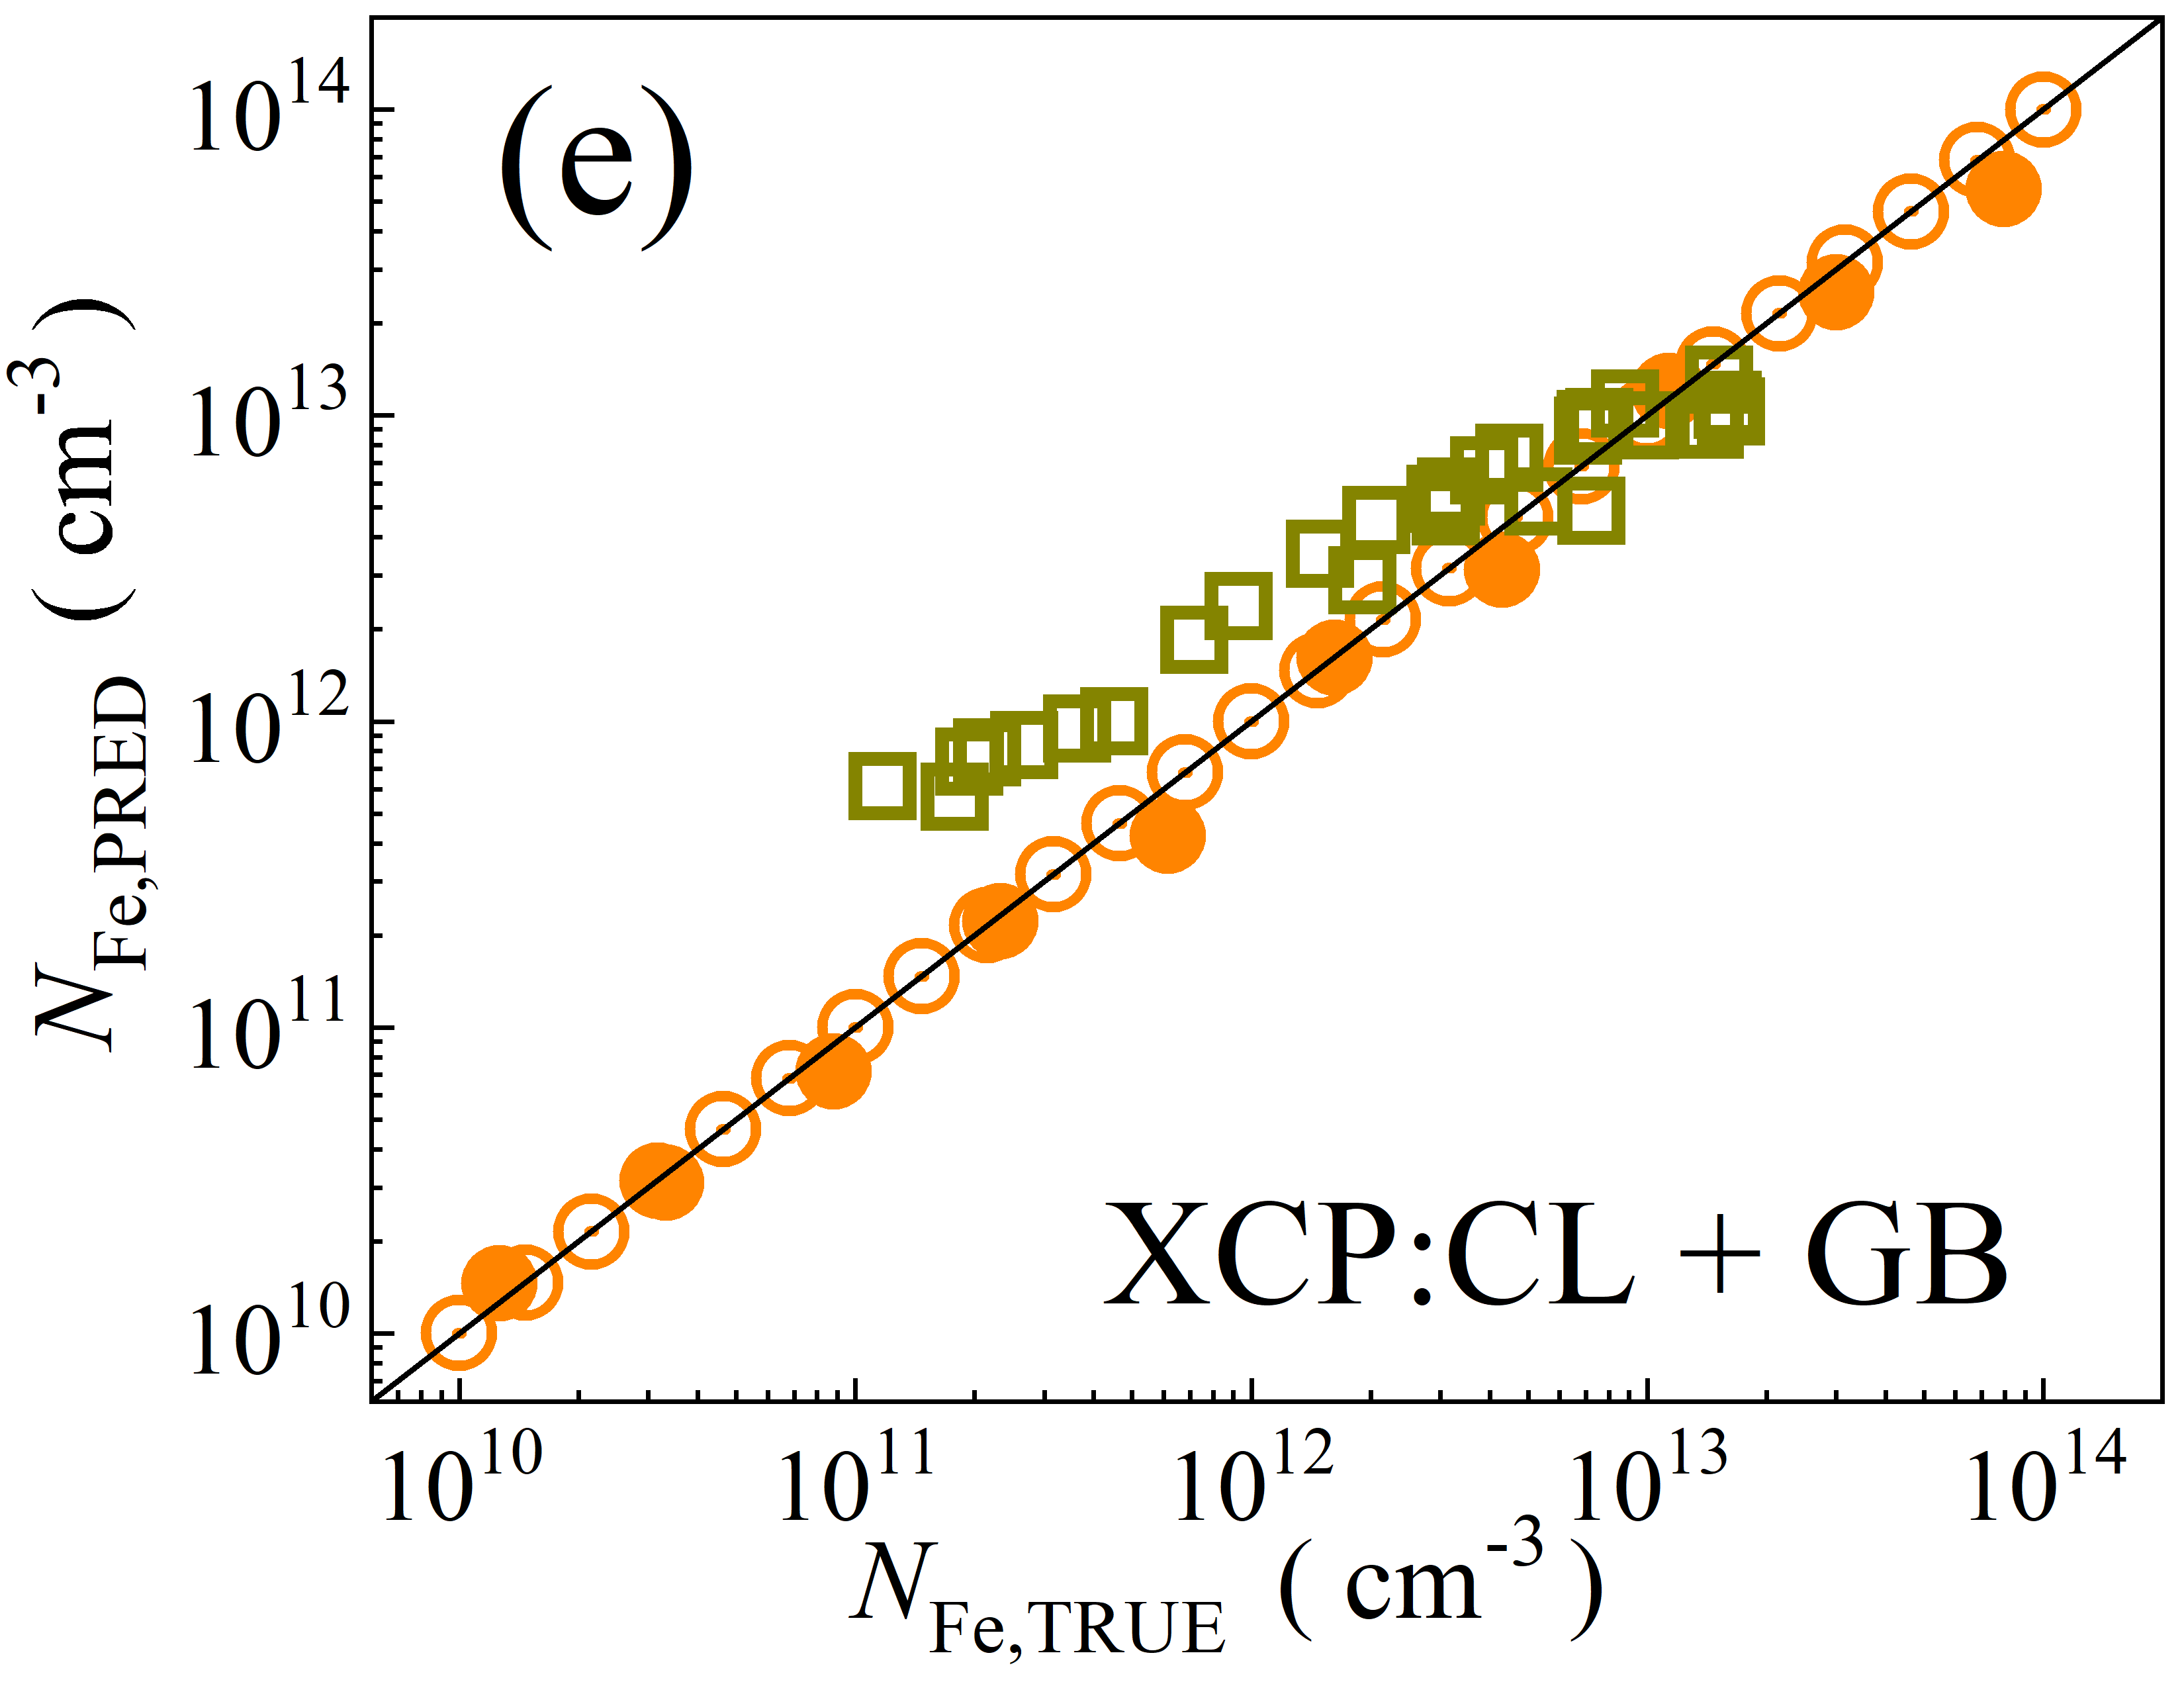
\includegraphics[width=0.33\textwidth]{Fig4e}
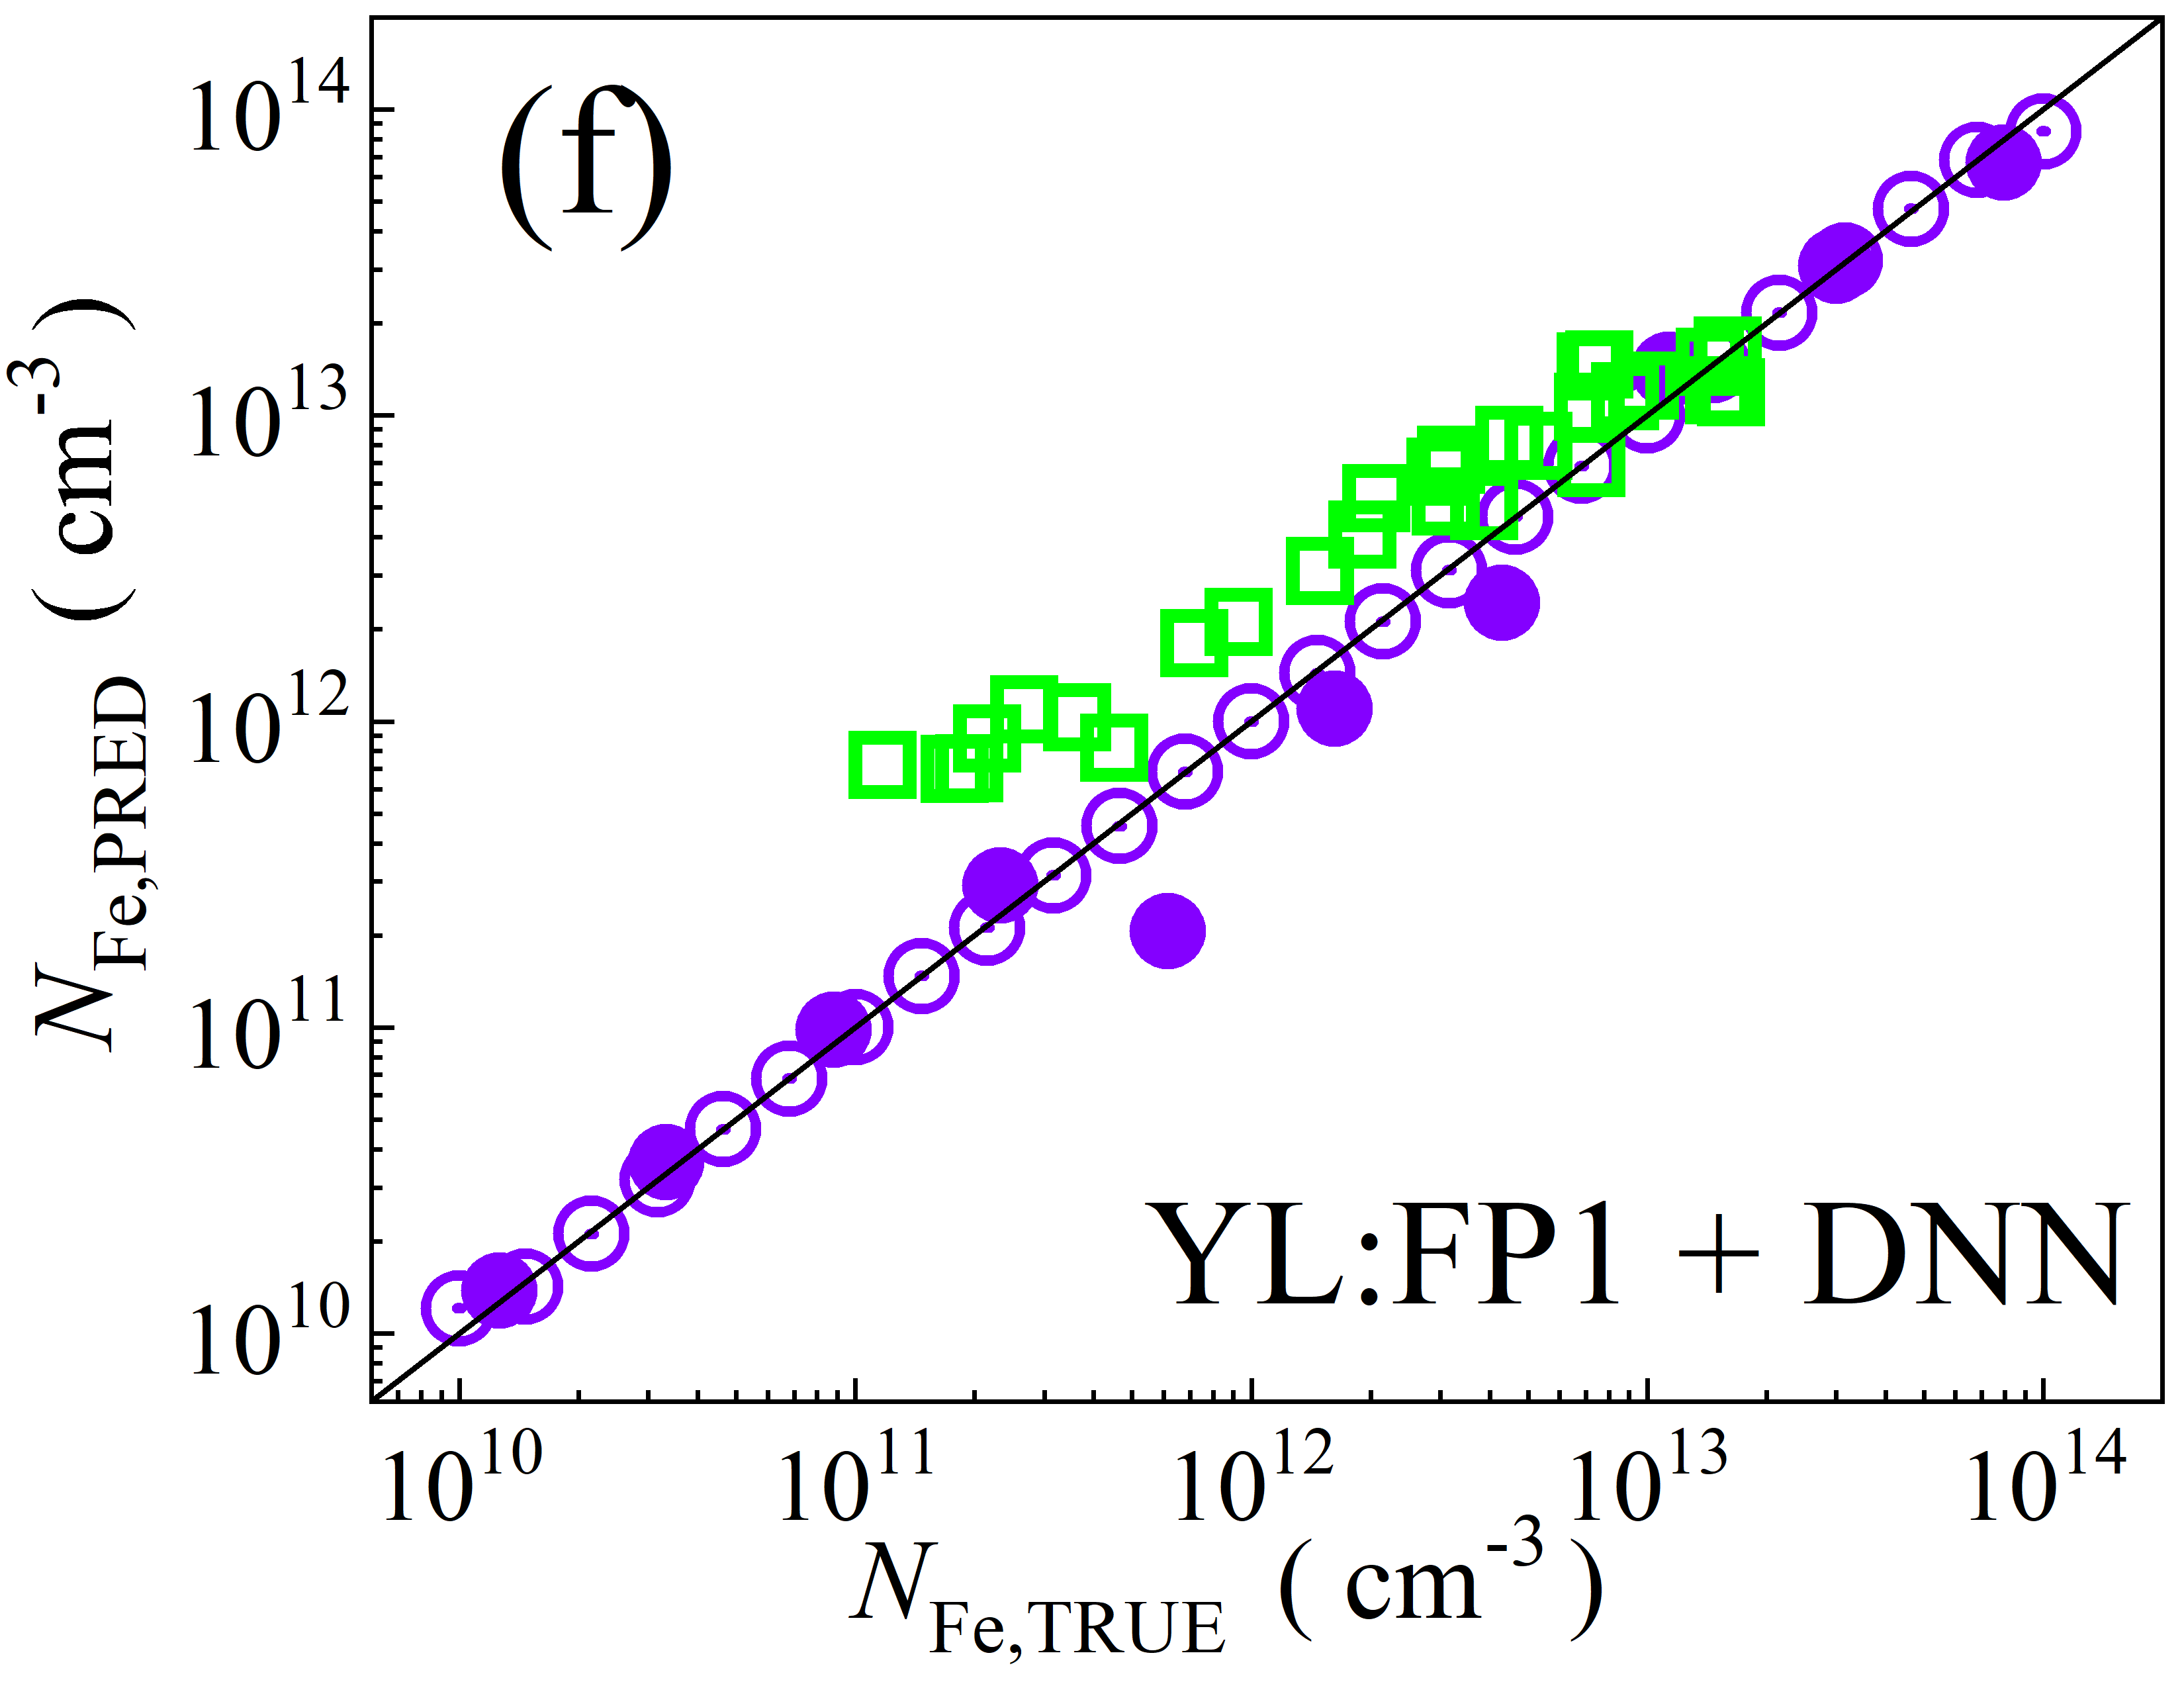
\includegraphics[width=0.33\textwidth]{Fig4f}
\caption{
Scatter plots compare the reference iron $N_\mathrm{Fe,TRUE}$ with ML-predicted values $N_\mathrm{Fe,PRED}$,
obtained using feature vectors extracted from various CV models combined with different regression algorithms
(specific models are indicated in the figures).
The ML models were trained on a simulated dataset.
The open circles correspond to the training phase,
while the filled circles and open squares correspond to the test phase, representing the simulated and experimental datasets, respectively.
The black lines are the identified lines serving as the references.
}\label{Fig4}
\end{figure*}

\Fref{Fig5} presents the MAPE and $R^2$ scores obtained when applying the models to the training dataset.
Although these metrics are sufficiently representative, the corresponding MedAPE and MSE values are provided in Figure~S2 (Supplementary Material).
The most notable observation from \Fref{Fig4} and \Fref{Fig5} is that,
despite the very limited size of the training dataset (25 samples),
most models demonstrate high training performance:
in many cases, the mean relative error is approximately 1\% or lower,
and it rarely exceeds 10\%. At the same time, the $R^2$ score drops below 0.980 in only 8 out of 87 cases.
It is also worth noting that the MedAPE values generally do not exceed the MAPE and are, in fact,
smaller in most instances (see Figure~S2).
These consistently high performance metrics indicate that
(i)~the wavelet transformation produced highly informative images that effectively encoded information about the Fe concentration,
and (ii)~the CV models successfully extracted features correlated with the concentration.

\begin{figure*}
\centering
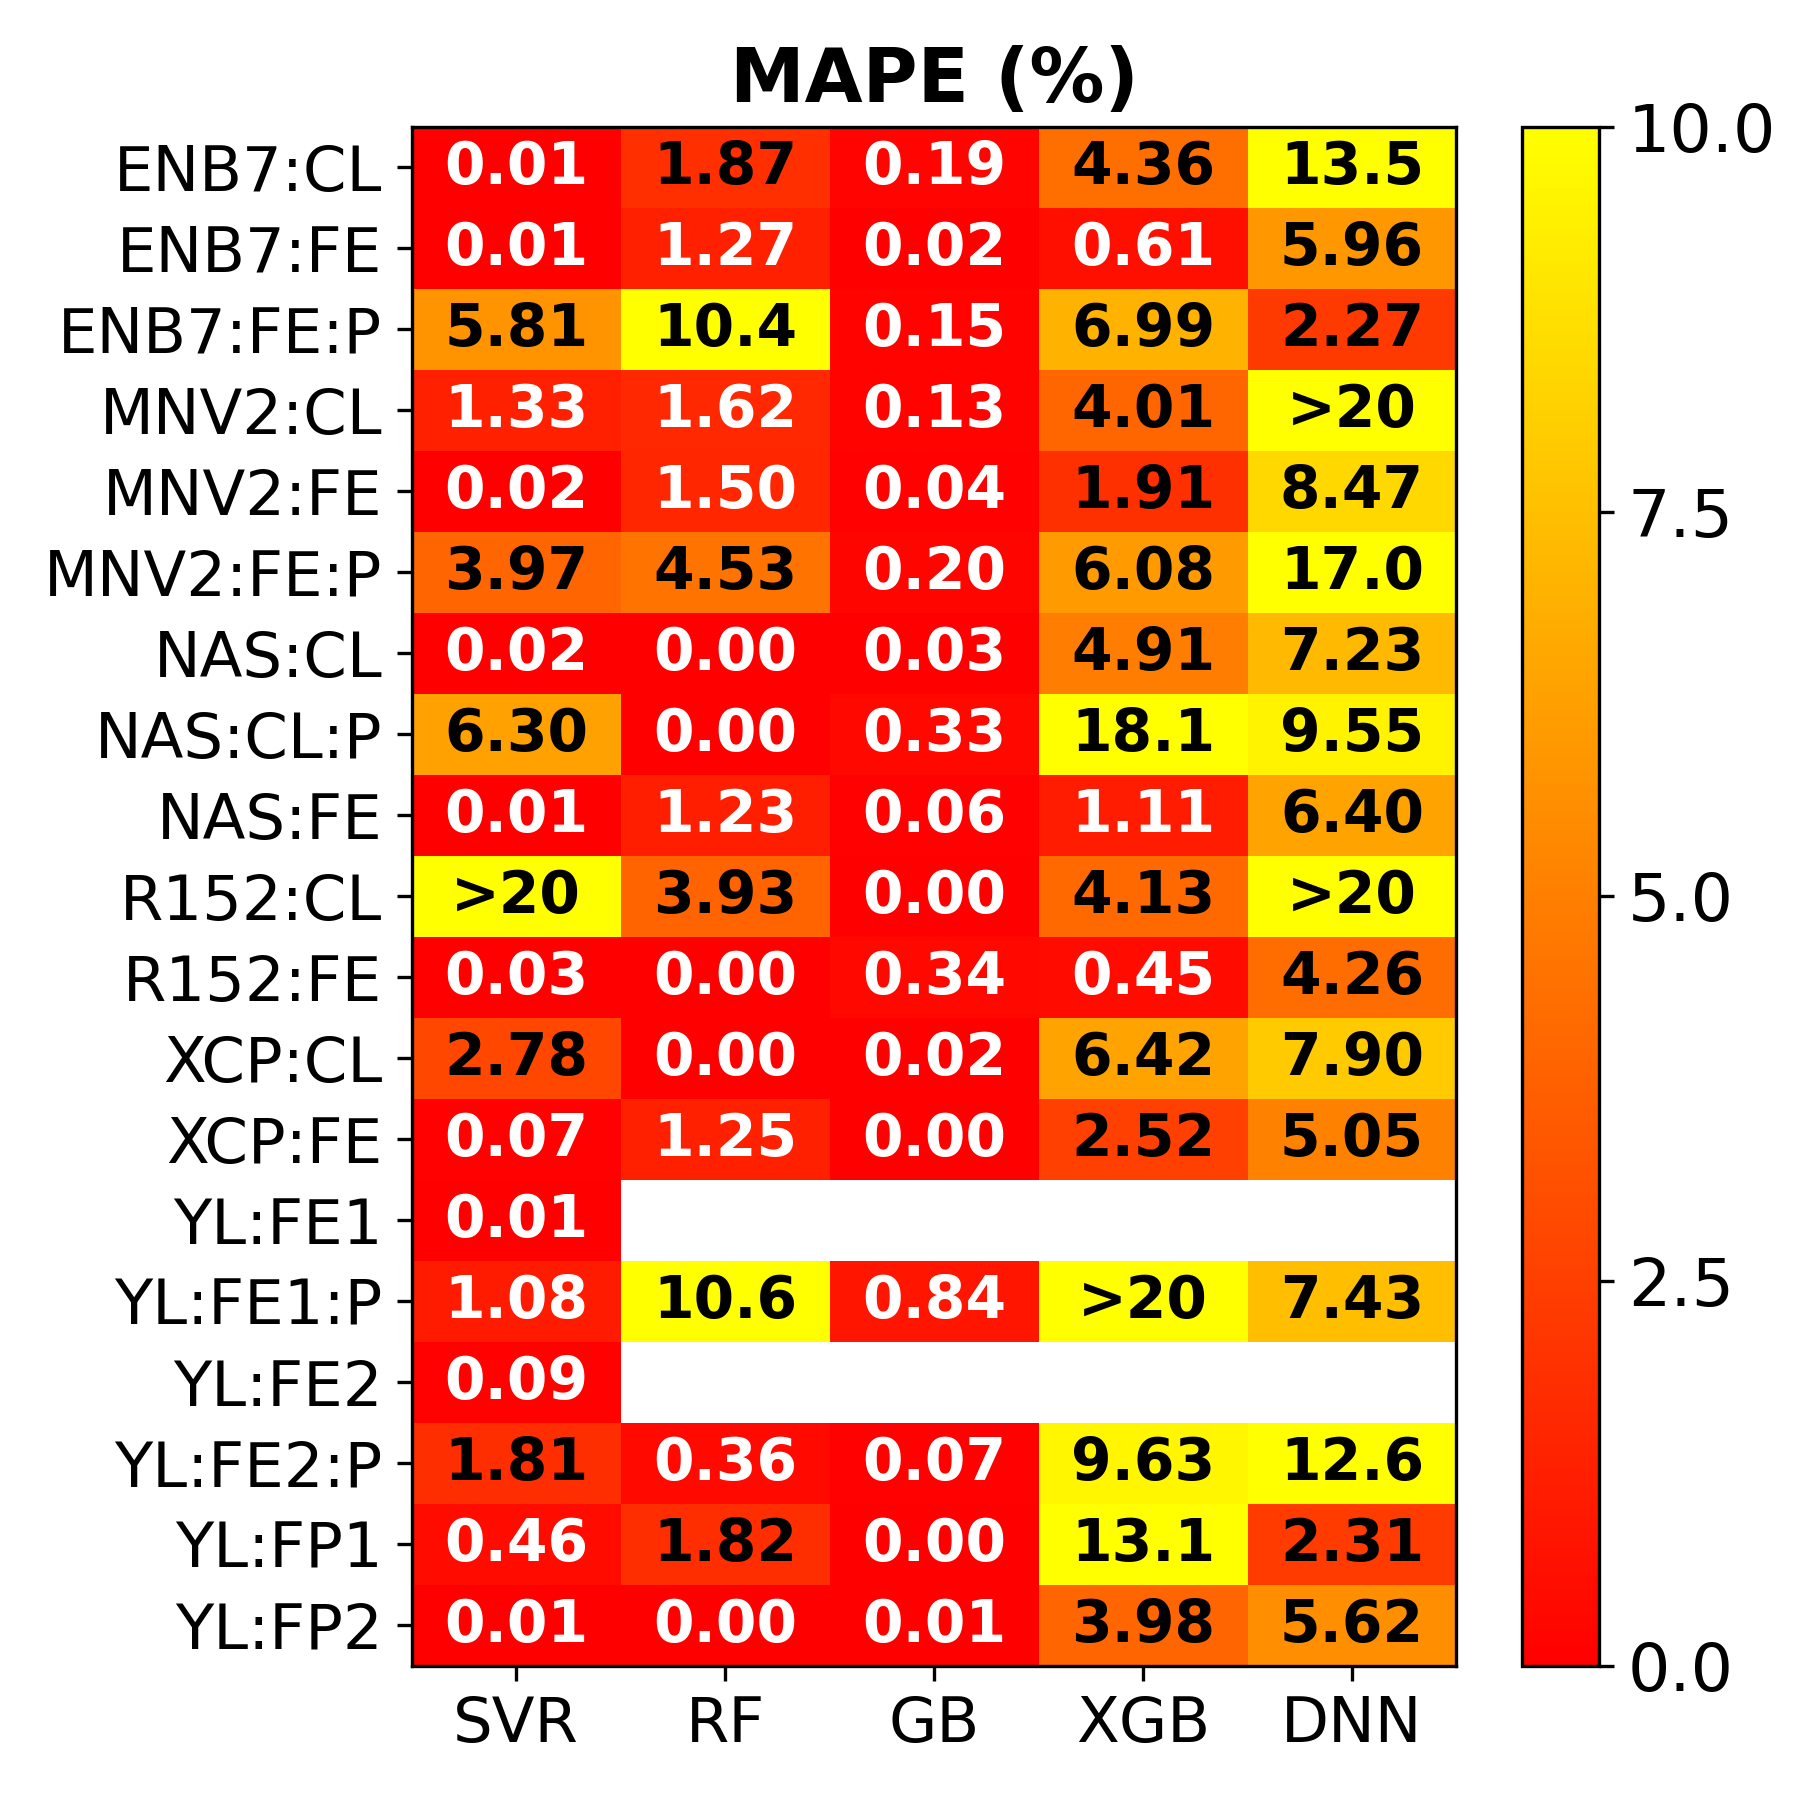
\includegraphics[width=0.35\textwidth]{Fig5a}
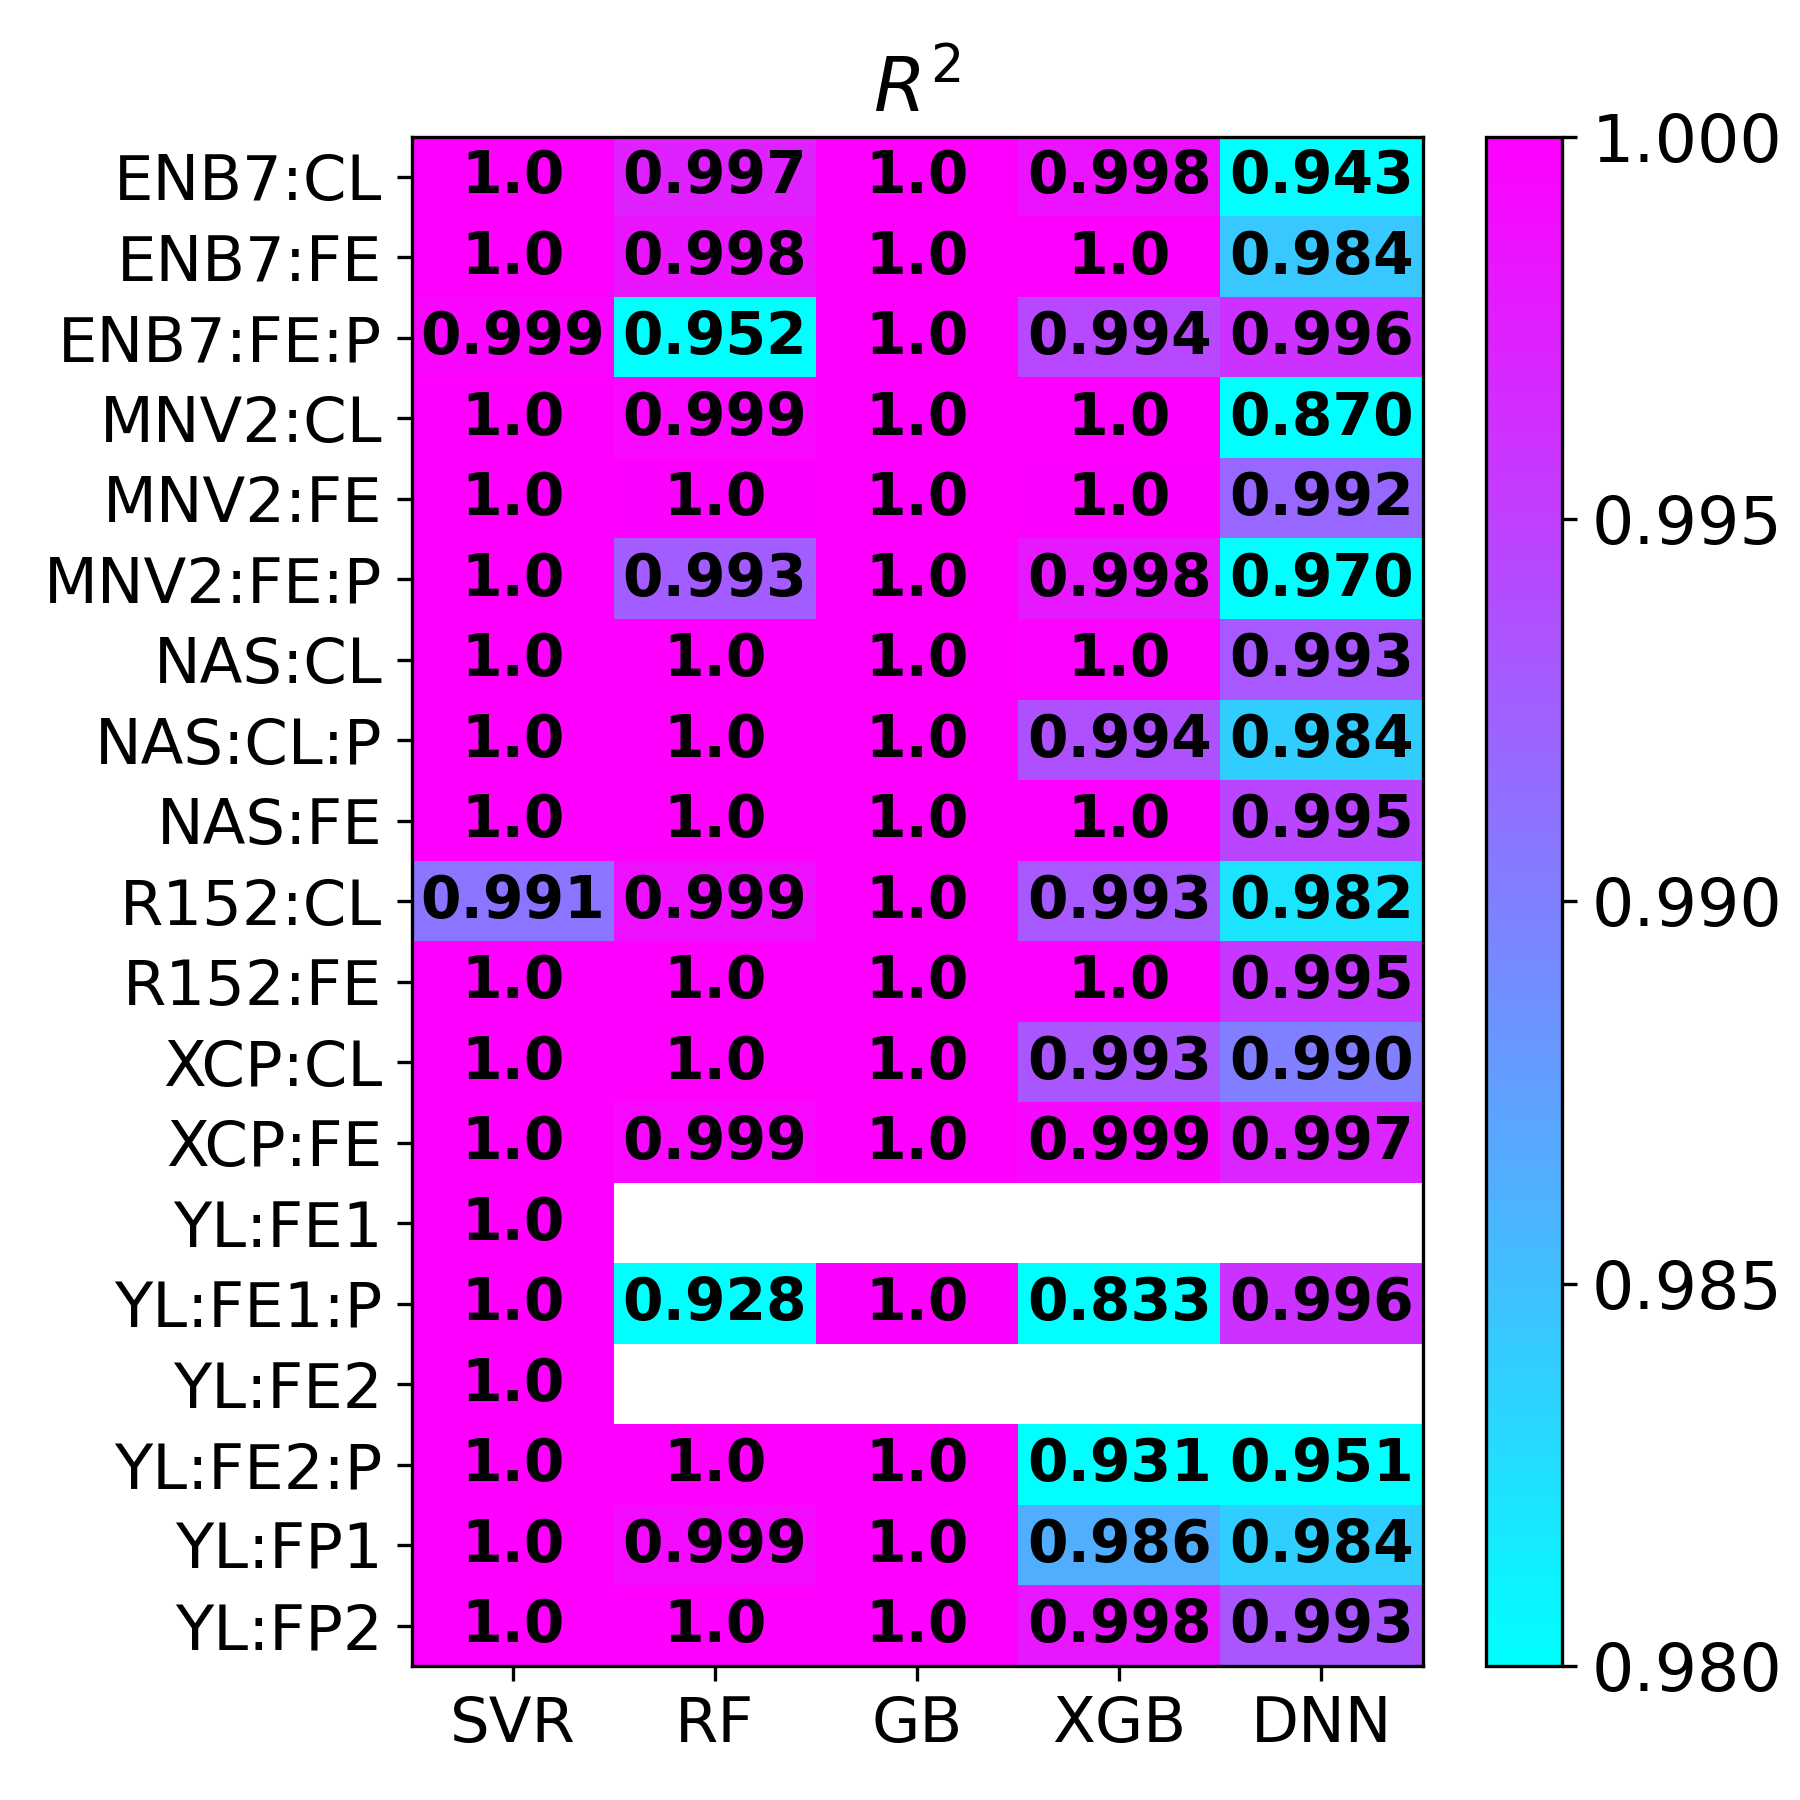
\includegraphics[width=0.35\textwidth]{Fig5b}
\caption{
Mean absolute percentage error (left panel) and coefficient of determination (right panel) for different combinations of CV models (vertical axis)
and regression models (horizontal axis) during the training phase. The models were trained on a simulated dataset.
}\label{Fig5}
\end{figure*}

Among the regression models, GB and SVR exhibited the best performance,
whereas the DNN produced the least favorable results.
This outcome is entirely consistent with expectations,
since both Gradient Boosting and Support Vector Regression are well known to perform effectively
when the number of samples is limited and the feature space exhibits a low noise level, as is characteristic of synthetic datasets.
In contrast, neural networks contain a large number of parameters and therefore do not tend to exhibit perfect generalization under such conditions.

Among the CV models, EfficientNetB7 and NASNetLarge demonstrated the best performance,
whereas ResNet152V2 and YOLOv4 showed the weakest results.
This discrepancy can be attributed to the fact that the former two are relatively modern architectures
specifically designed to extract generalizable features and are therefore well suited to wavelet spectrograms,
which are characterized by a multi-scale structure.
In contrast, ResNet152V2 is primarily optimized for object classification, whereas YOLO is less effective for regression
tasks involving global image patterns, as it focuses on localized object detection.

It is also evident that using class probabilities as descriptors degrades prediction quality
compared with the cases where image features are employed directly.
This indicates that the internal feature maps of CNN models provide a more informative representation of visual patterns,
enabling the regressor to establish a stronger relationship with concentration.
Moreover, the application of PCA, even though it retains 99.9\% of the variance, results in reduced predictive accuracy.
This observation suggests that the image patterns associated with variations in iron concentration may constitute
only a minor portion of the overall data variance.

The ability of models to achieve high accuracy on the training set is a necessary prerequisite for effective performance on unseen data;
however, it does not guarantee reliable prediction outcomes.
Consequently, evaluation on an independent test set is essential.
This step becomes particularly critical when the training set is small, as the test results provide the primary evidence of model generalizability.
\Fref{Fig4} and \Fref{Fig6} present the prediction results obtained for the test set generated from synthetic data
(more detailed versions are available in Figures~S1 and S3 of the Supplementary Material).
As expected, prediction performance declined; however, the reduction in accuracy varied across the regression algorithms.
Specifically, this degradation was least pronounced for the DNN, which achieved the best overall performance.
The poorest metrics were obtained for RF and GB, whereas SVR and XGB performed slightly worse than the DNN but with a relatively small margin.
This behavior can be attributed to the DNN’s ability to approximate continuous dependencies smoothly.
In contrast to GB and RF, which rely on the formation of local decision rules,
neural networks construct a continuous surface in the feature space.
This property enhances interpolation for iron concentration values not represented in the training data.
From this perspective, XGB and SVR occupy an intermediate position, explaining their slightly lower performance relative to the DNN.

\begin{figure*}
\centering
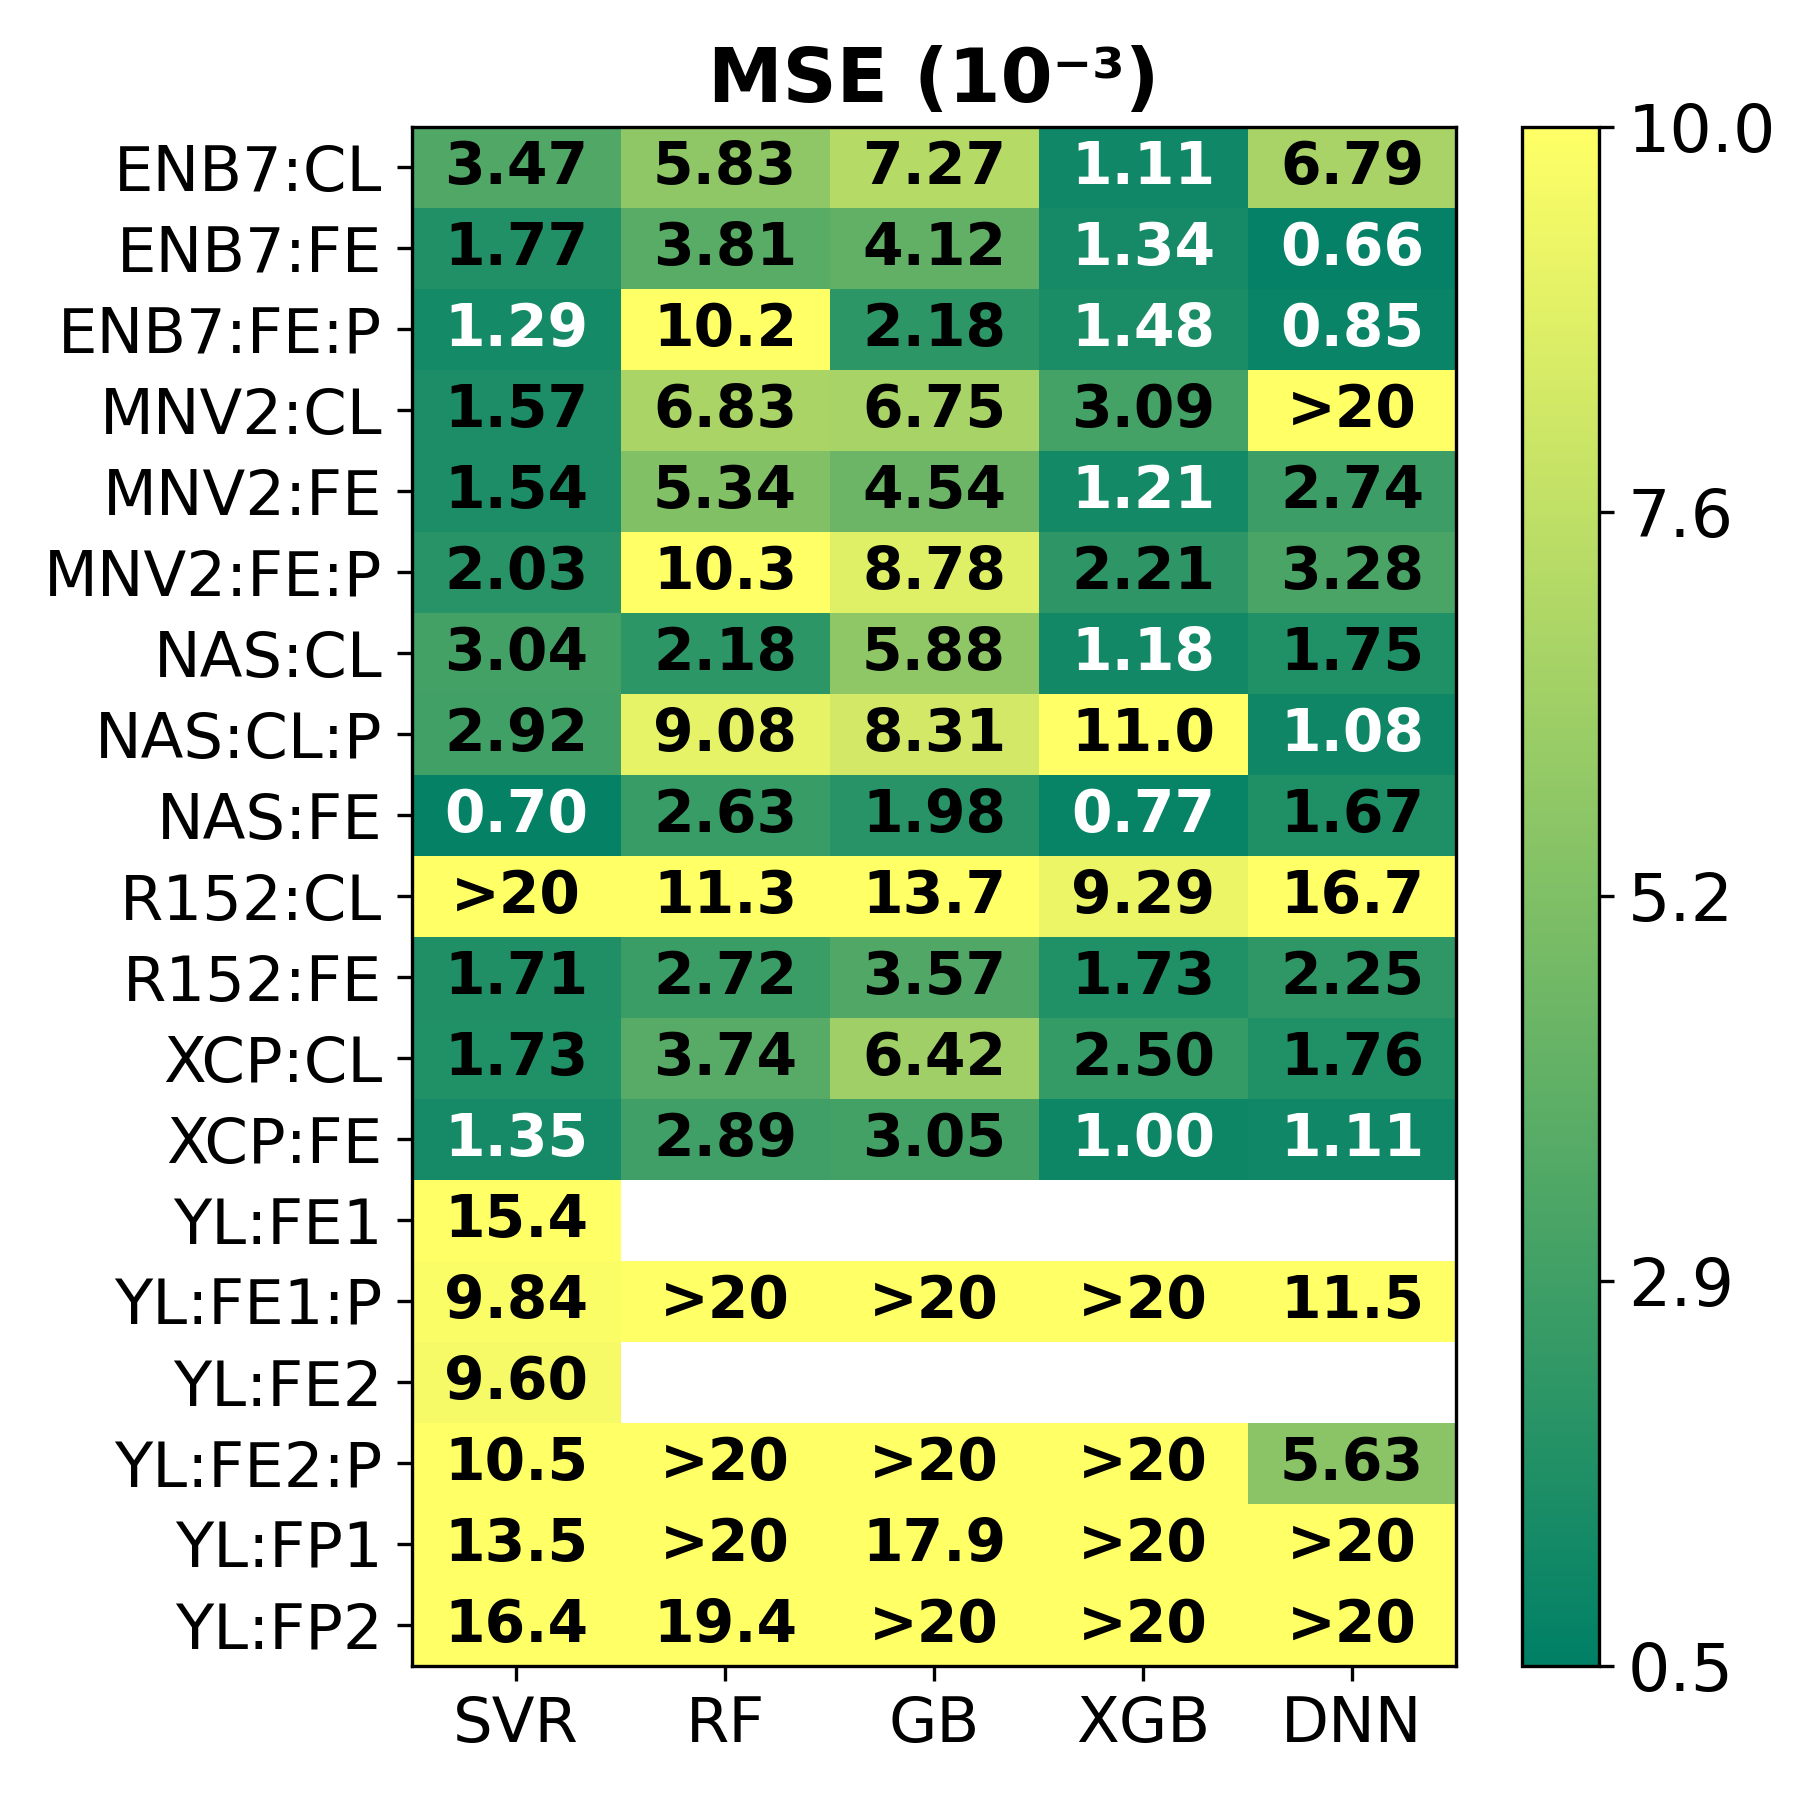
\includegraphics[width=0.35\textwidth]{Fig6a}
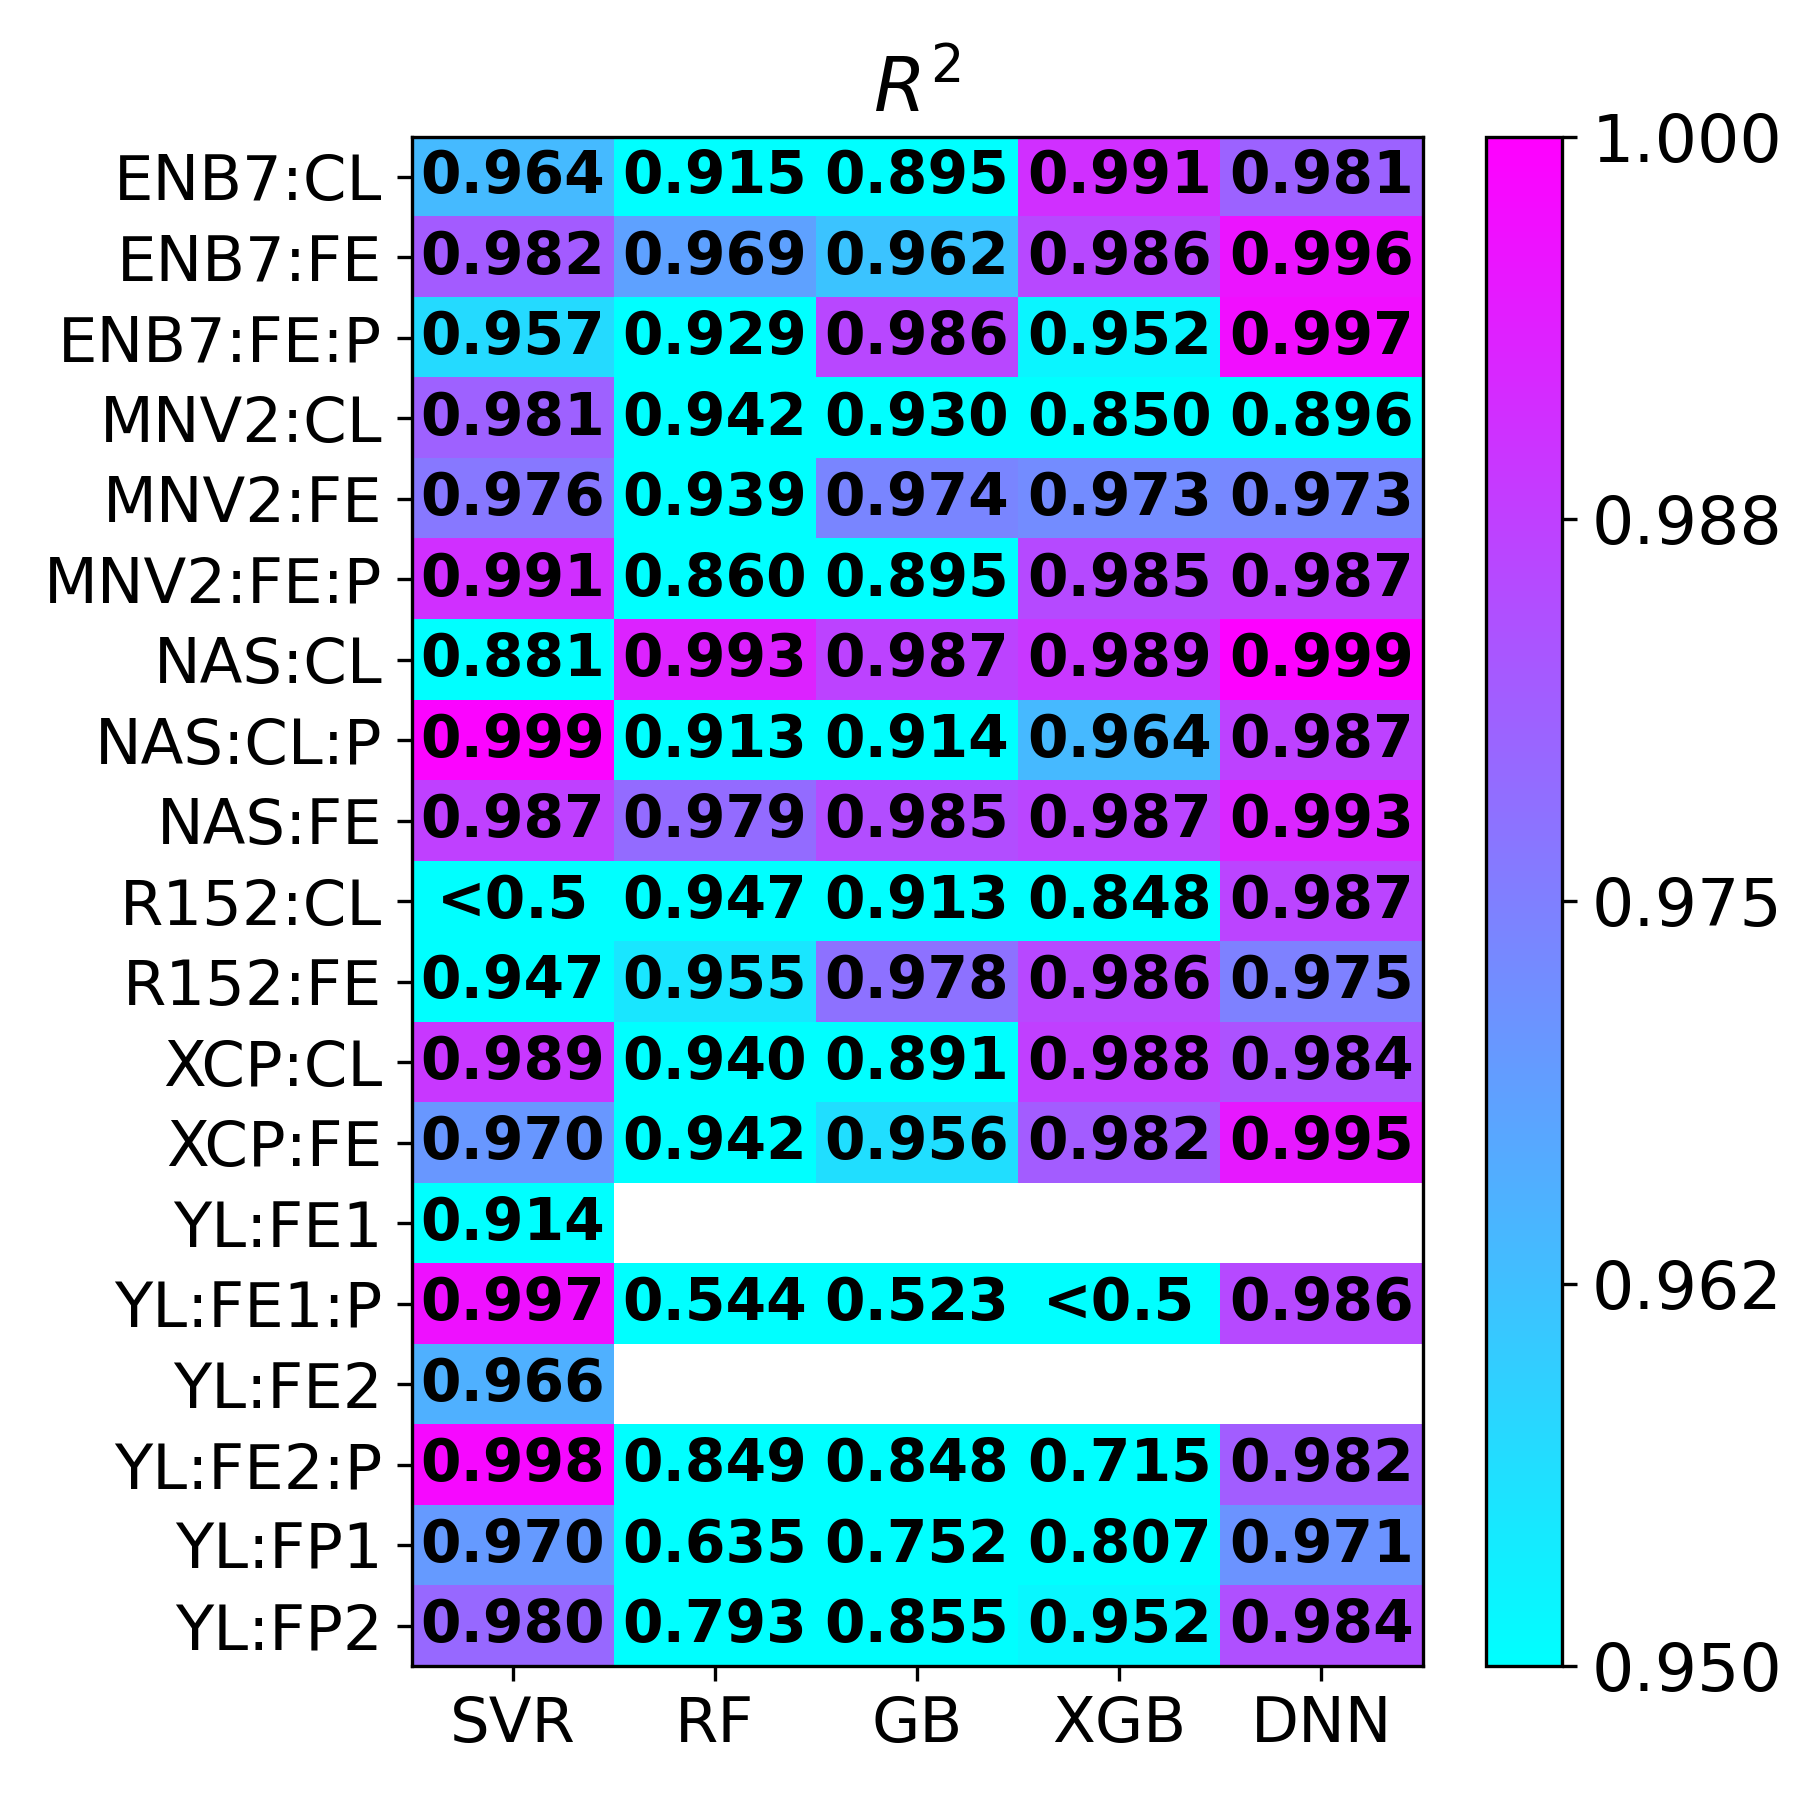
\includegraphics[width=0.35\textwidth]{Fig6b}
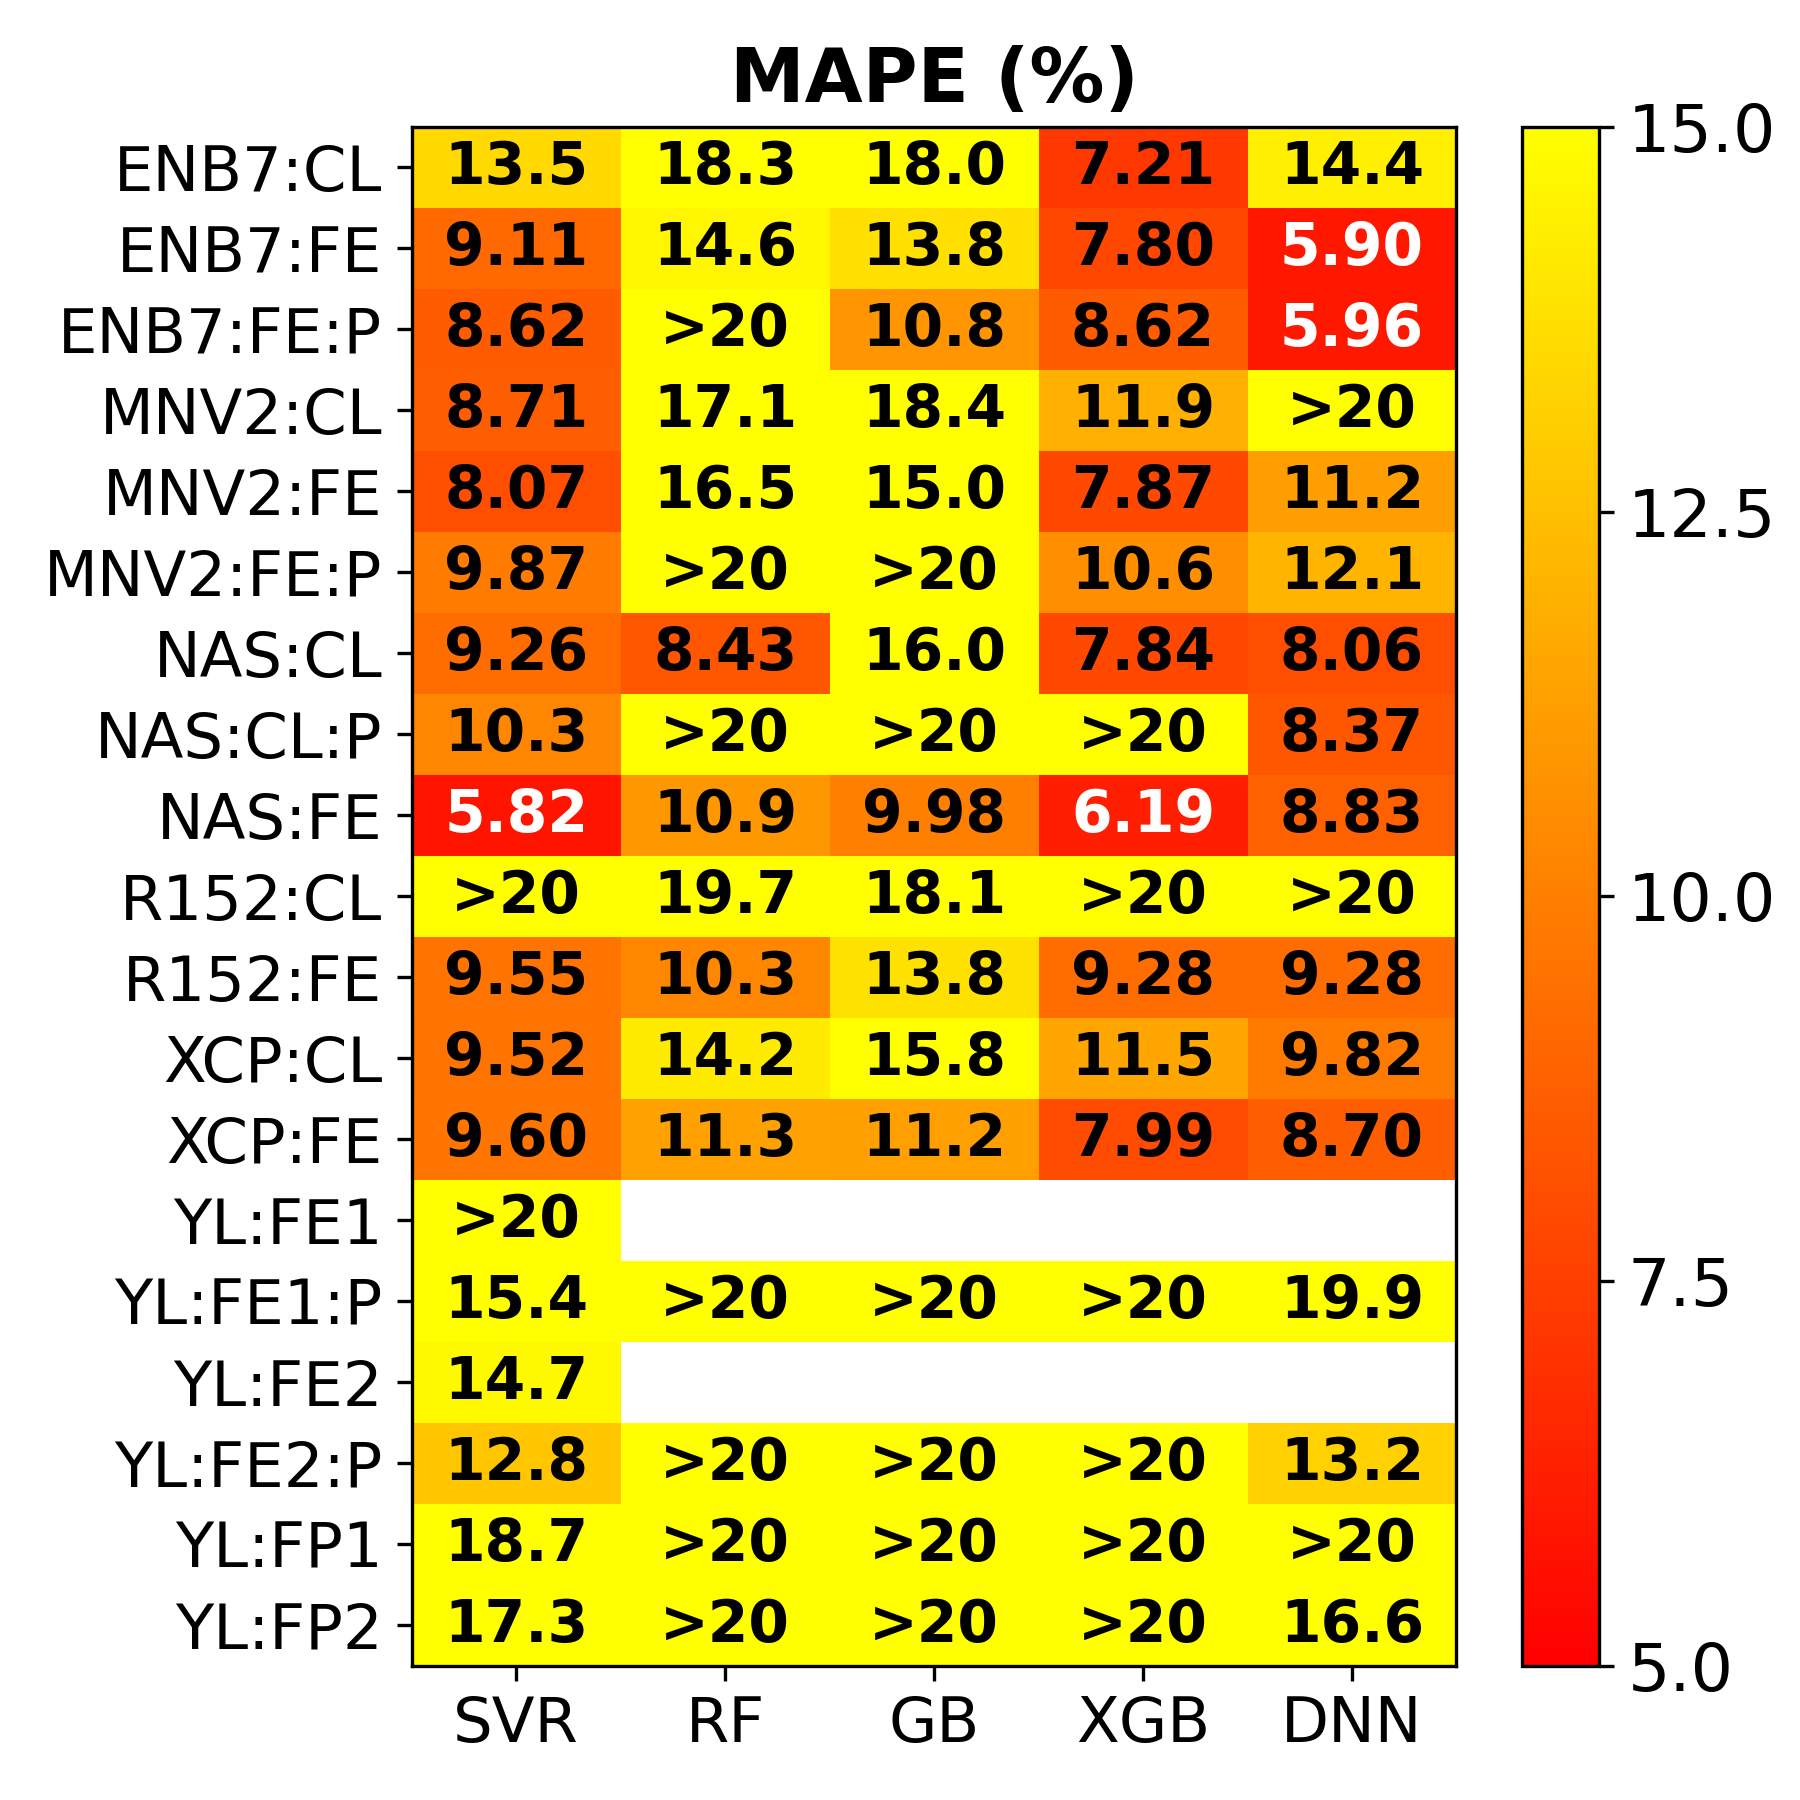
\includegraphics[width=0.35\textwidth]{Fig6c}
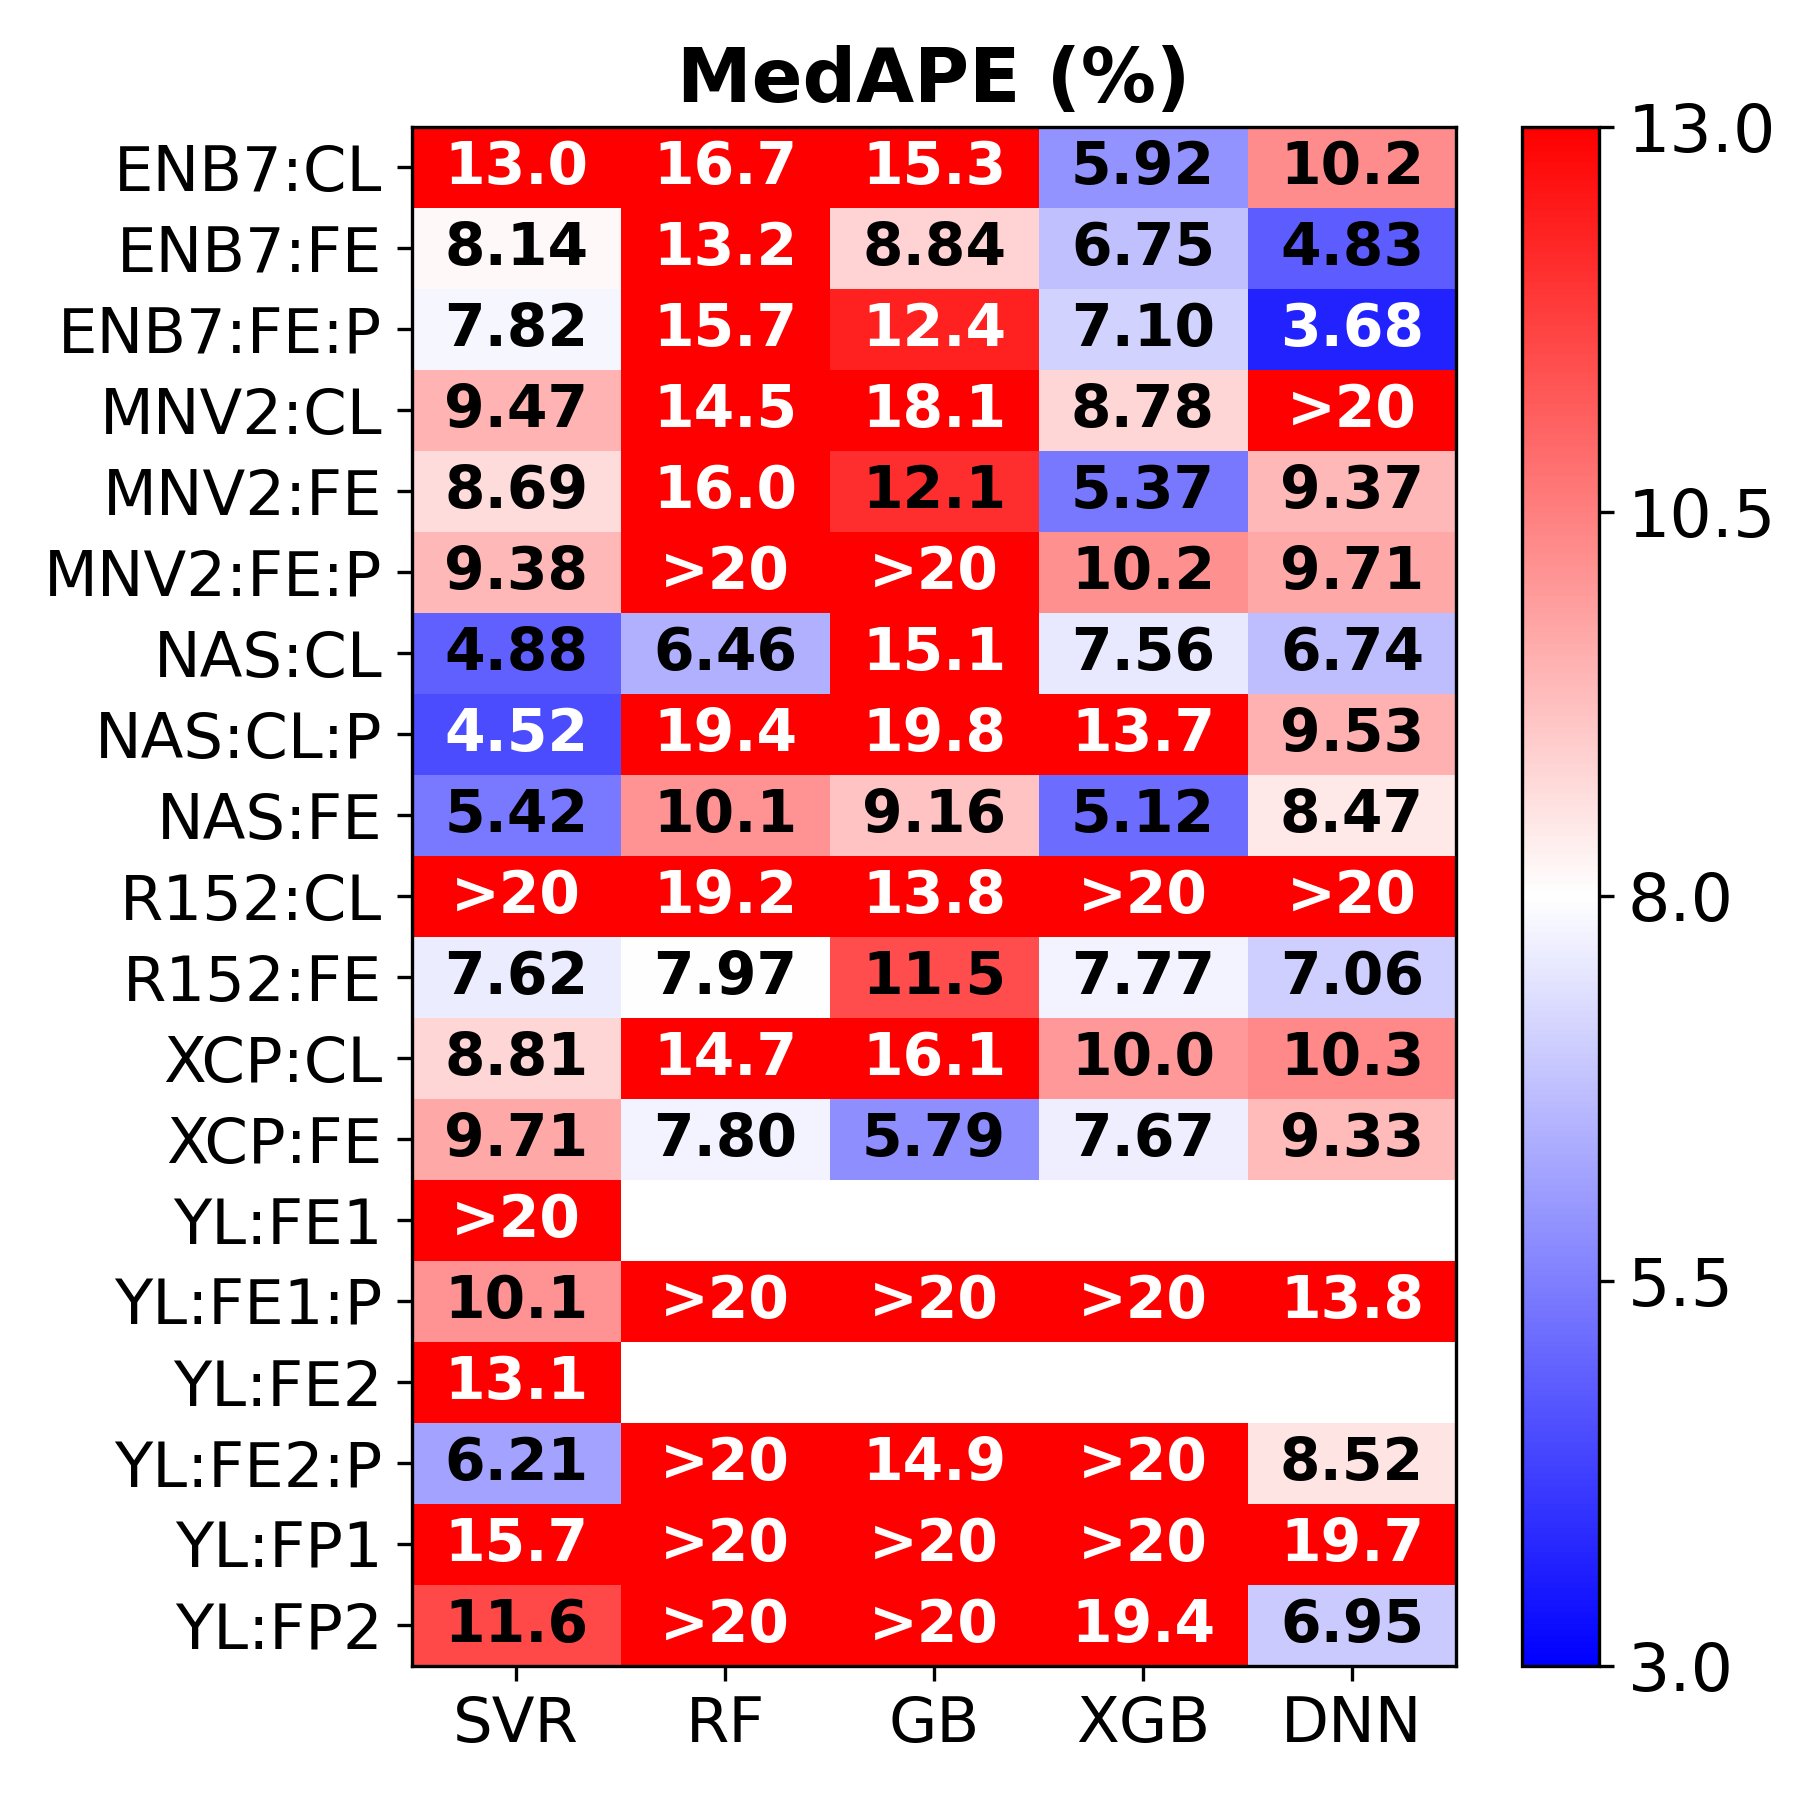
\includegraphics[width=0.35\textwidth]{Fig6d}
\caption{
Mean squared error, coefficient of determination, mean absolute percentage error, and median absolute percentage error
for different combinations of CV models (vertical axis) and regression models (horizontal axis)
during the test phase with simulated dataset.
The models were trained on a simulated training dataset.
}\label{Fig6}
\end{figure*}


As shown, the relative performance of the computer vision models on the simulated test dataset remained consistent,
with no change in the top- and bottom-performing architectures.
Specifically, EfficientNetB7 and NASNetLarge yielded the most favorable results,
confirming their effectiveness in extracting wavelet image features relevant for concentration prediction.
In contrast, ResNet152V2 and YOLOv4 produced the least satisfactory outcomes.
A notable exception arises in configurations where YOLOv4 features from two layers are combined with either a DNN or SVR.
In these cases, performance metrics were considerably improved.
This enhancement suggests that the use of a larger number of features enabled the capture of more diverse patterns,
which, when coupled with flexible regressors, partially mitigated the limitations observed in the standalone YOLO model.

Interestingly, the PCA application to the test set did not substantially degrade performance;
in certain cases, it even produced slight improvements.
This indicates that PCA is not universally detrimental, although the resulting gains are generally marginal and unpredictable.
Moreover, the differences in metrics between models using class probabilities and those employing raw image features
were less pronounced than observed for the training dataset.
Nevertheless, uncompressed feature representations consistently maintained a performance advantage.

The top-performing model combinations were identified as follows:
ENB7:FE+DNN (MAPE~=~5.90\%,
MedAPE~=~4.83\%,
$R^2= 0.996$),
ENB7:FE:P+DNN
(MAPE~=~5.96\%,
MedAPE~=~3.68\%,
$R^2 = 0.997$),
NAS:FE+SVR
(MAPE~=~5.82\%,
MedAPE~=~5.42\%,
$R^2 = 0.987$),
NAS:FE+XGB
(MAPE~=~6.19\%,
MedAPE~=~5.12\%,
$R^2 = 0.987$),
and NAS:CL:P+SVR
(MAPE~=~10.3\%,
MedAPE~=~4.52\%,
$R^2 = 0.999$).
These results correspond to exceptionally high absolute performance metrics,
providing clear evidence that the models effectively capture
the underlying relationship between the wavelet-based images and the iron concentration.

Having established the effectiveness of the models on the simulated test dataset,
we next evaluated their performance on experimental measurements.
This step is critical for assessing the generalizability of the models to real-world data,
where additional sources of noise and variability may be present.
By comparing the results obtained from experimental data with those from the simulated dataset,
it becomes possible to identify potential limitations of the models
and to confirm whether the features extracted from wavelet spectrograms remain informative under practical conditions.
\Fref{Fig7}a and \Fref{Fig7}b show the performance metrics of models trained on synthetic data when applied to experimental measurements.
The relationship between predicted and actual concentrations is illustrated in \Fref{Fig4}, with additional results provided in Figures S1 and S4.
As observed, the mean and median prediction errors fall within the (15–25)\% range for only a limited number of configurations,
specifically certain combinations of EfficientNetB7 or NASNetLarge with DNN or SVR.
Although this outcome is not catastrophic, considering the approximately 10\% inherent experimental error in $N_\mathrm{Fe}$ determination,
it falls short of ideal expectations.
At the same time, the $R^2$ metric remains acceptably high.
Further analysis (\Fref{Fig4}) indicates that the prediction error depends on the iron concentration level:
the relationship between $N_\mathrm{Fe,PRED}$ and $N_\mathrm{Fe,TRUE}$ is linear on a logarithmic scale,
but its slope deviates from the line of unity.
This observation suggests a systematic prediction bias rather than a complete loss of correlation,
implying that the models are capable of capturing relative differences in concentration but do not accurately predict absolute values.


\begin{figure*}
\centering
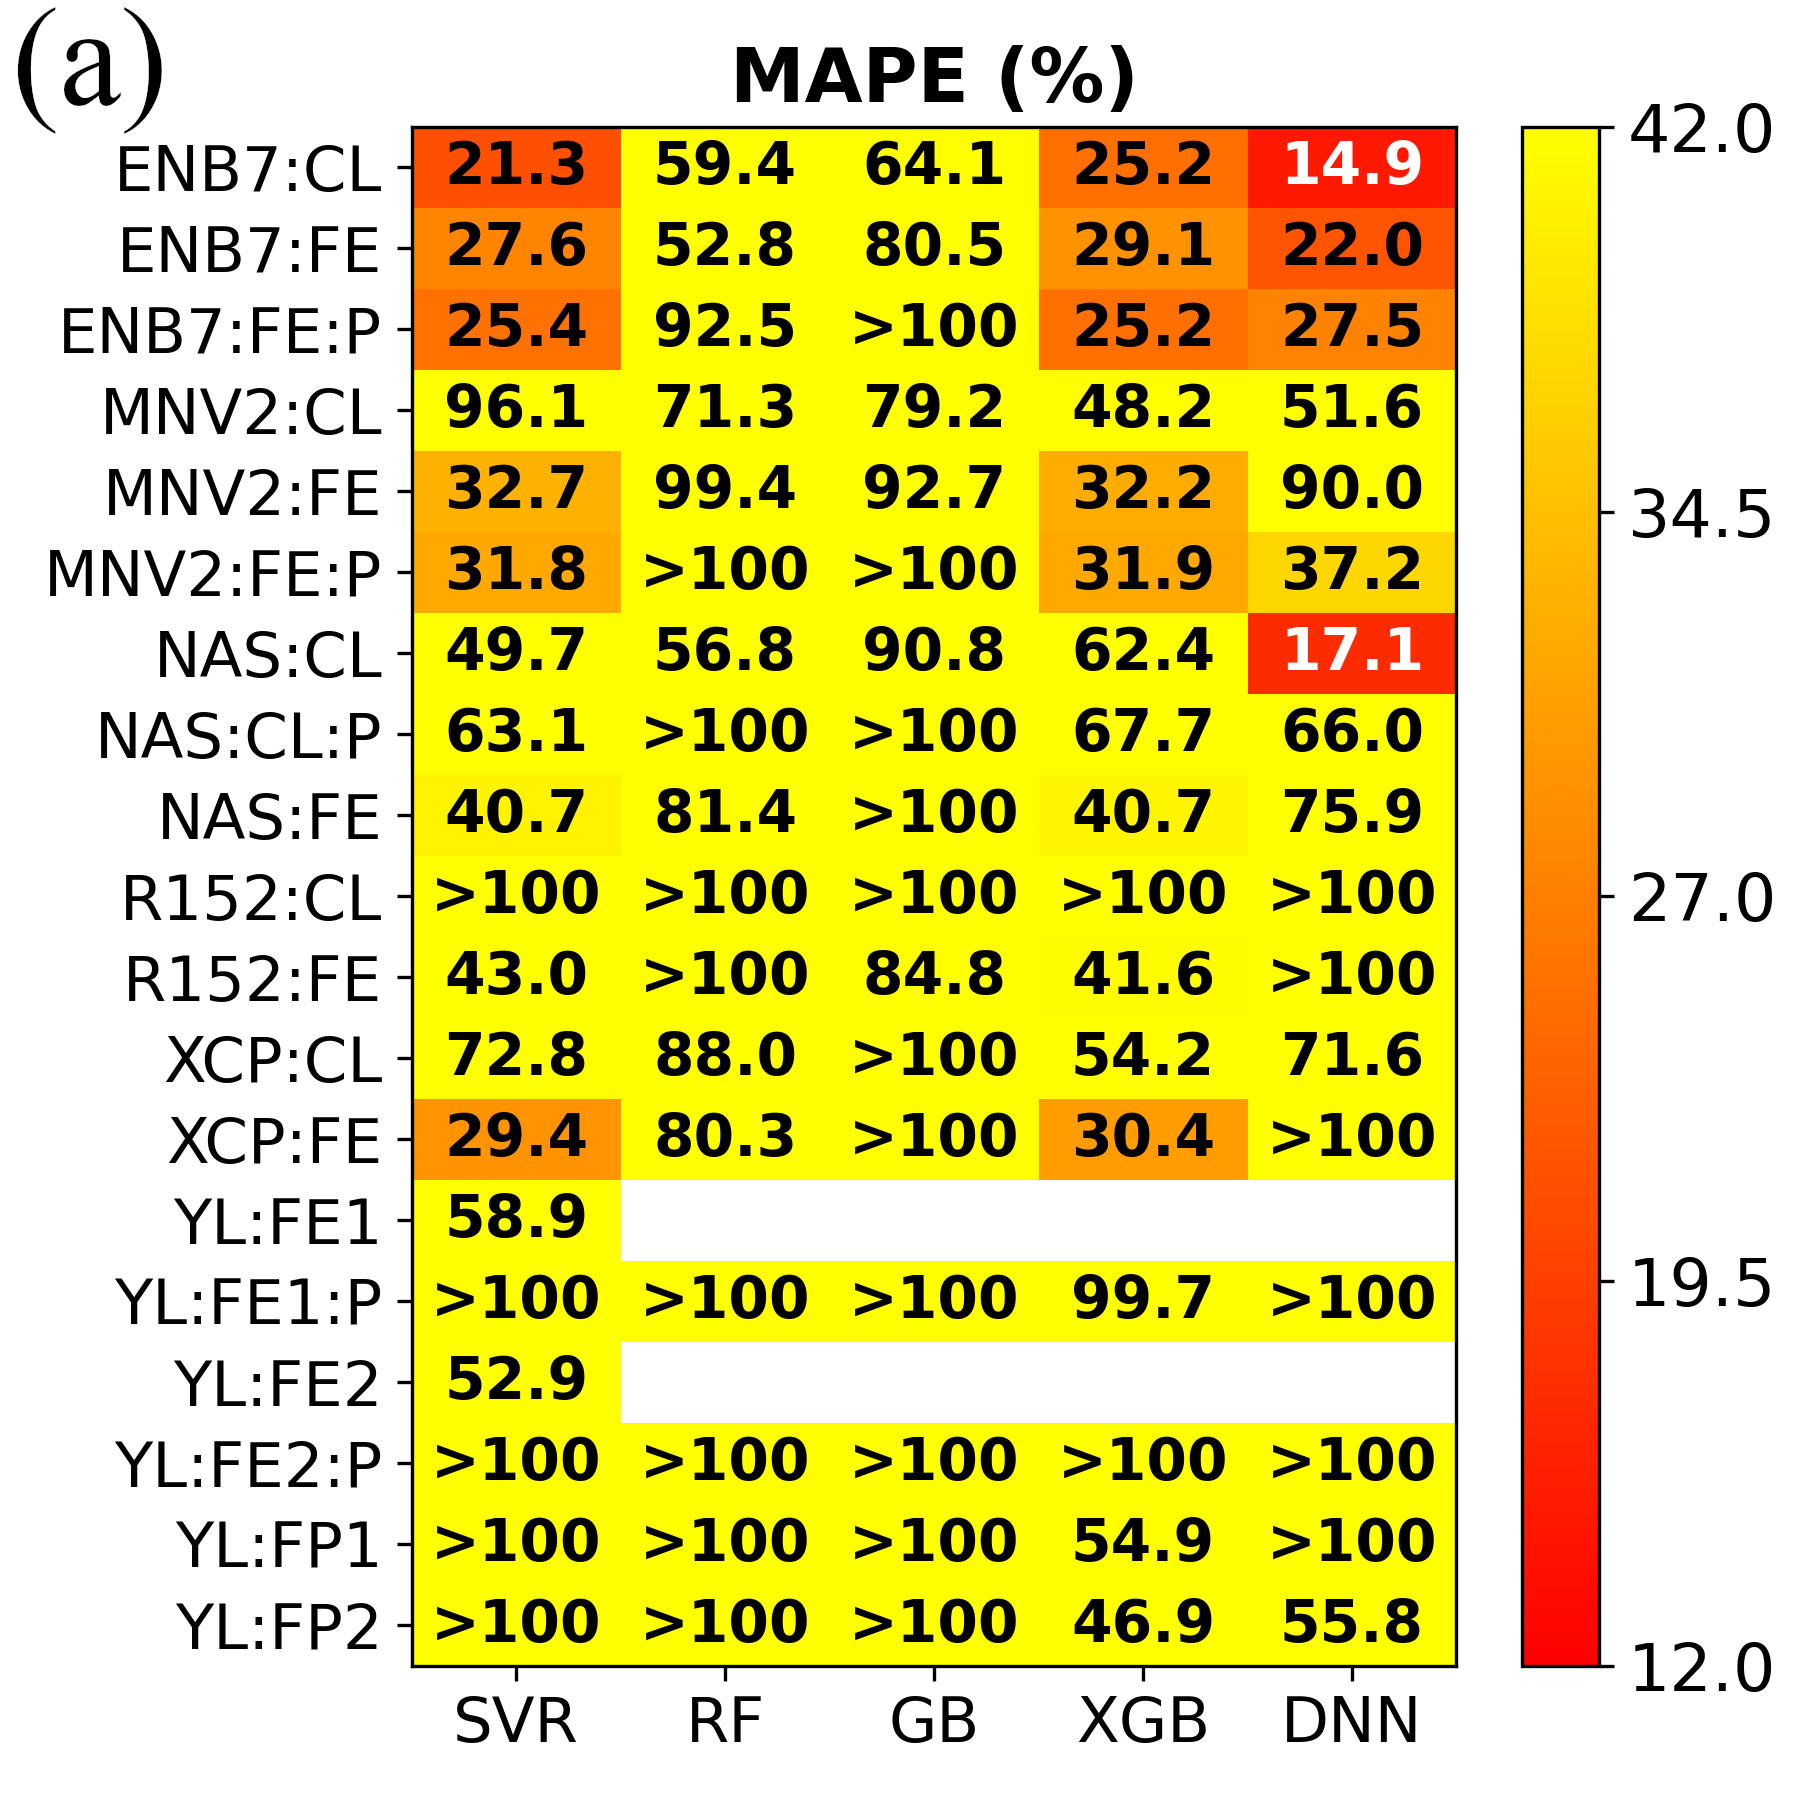
\includegraphics[width=0.35\textwidth]{Fig7a}
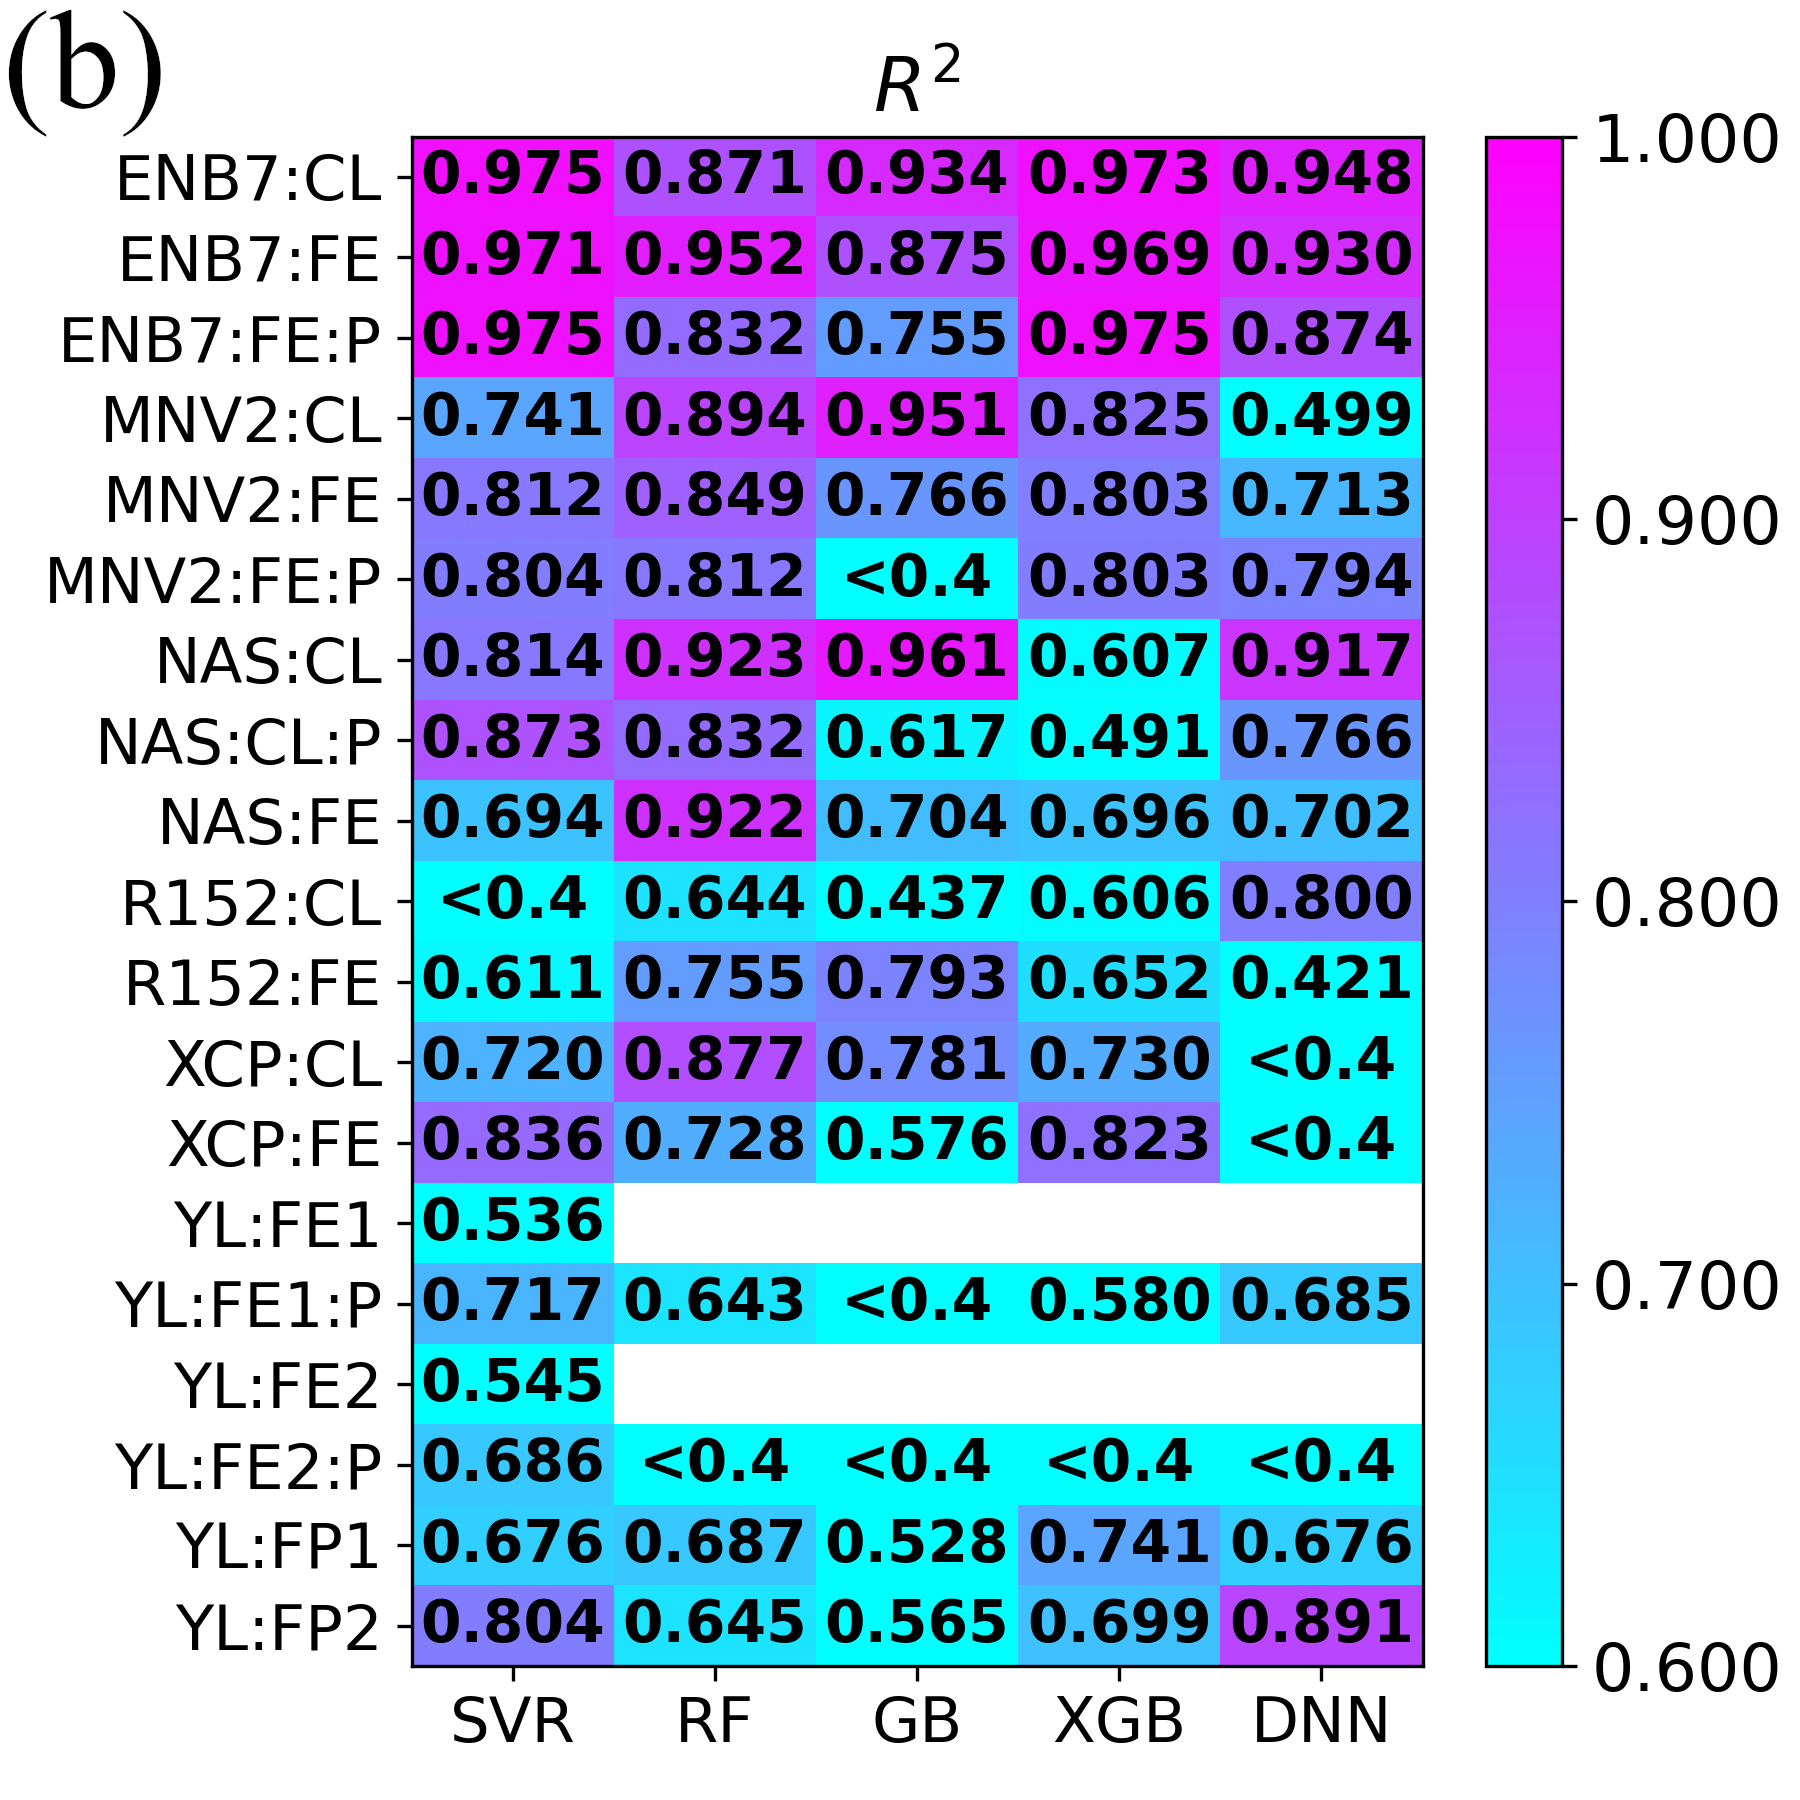
\includegraphics[width=0.35\textwidth]{Fig7b}
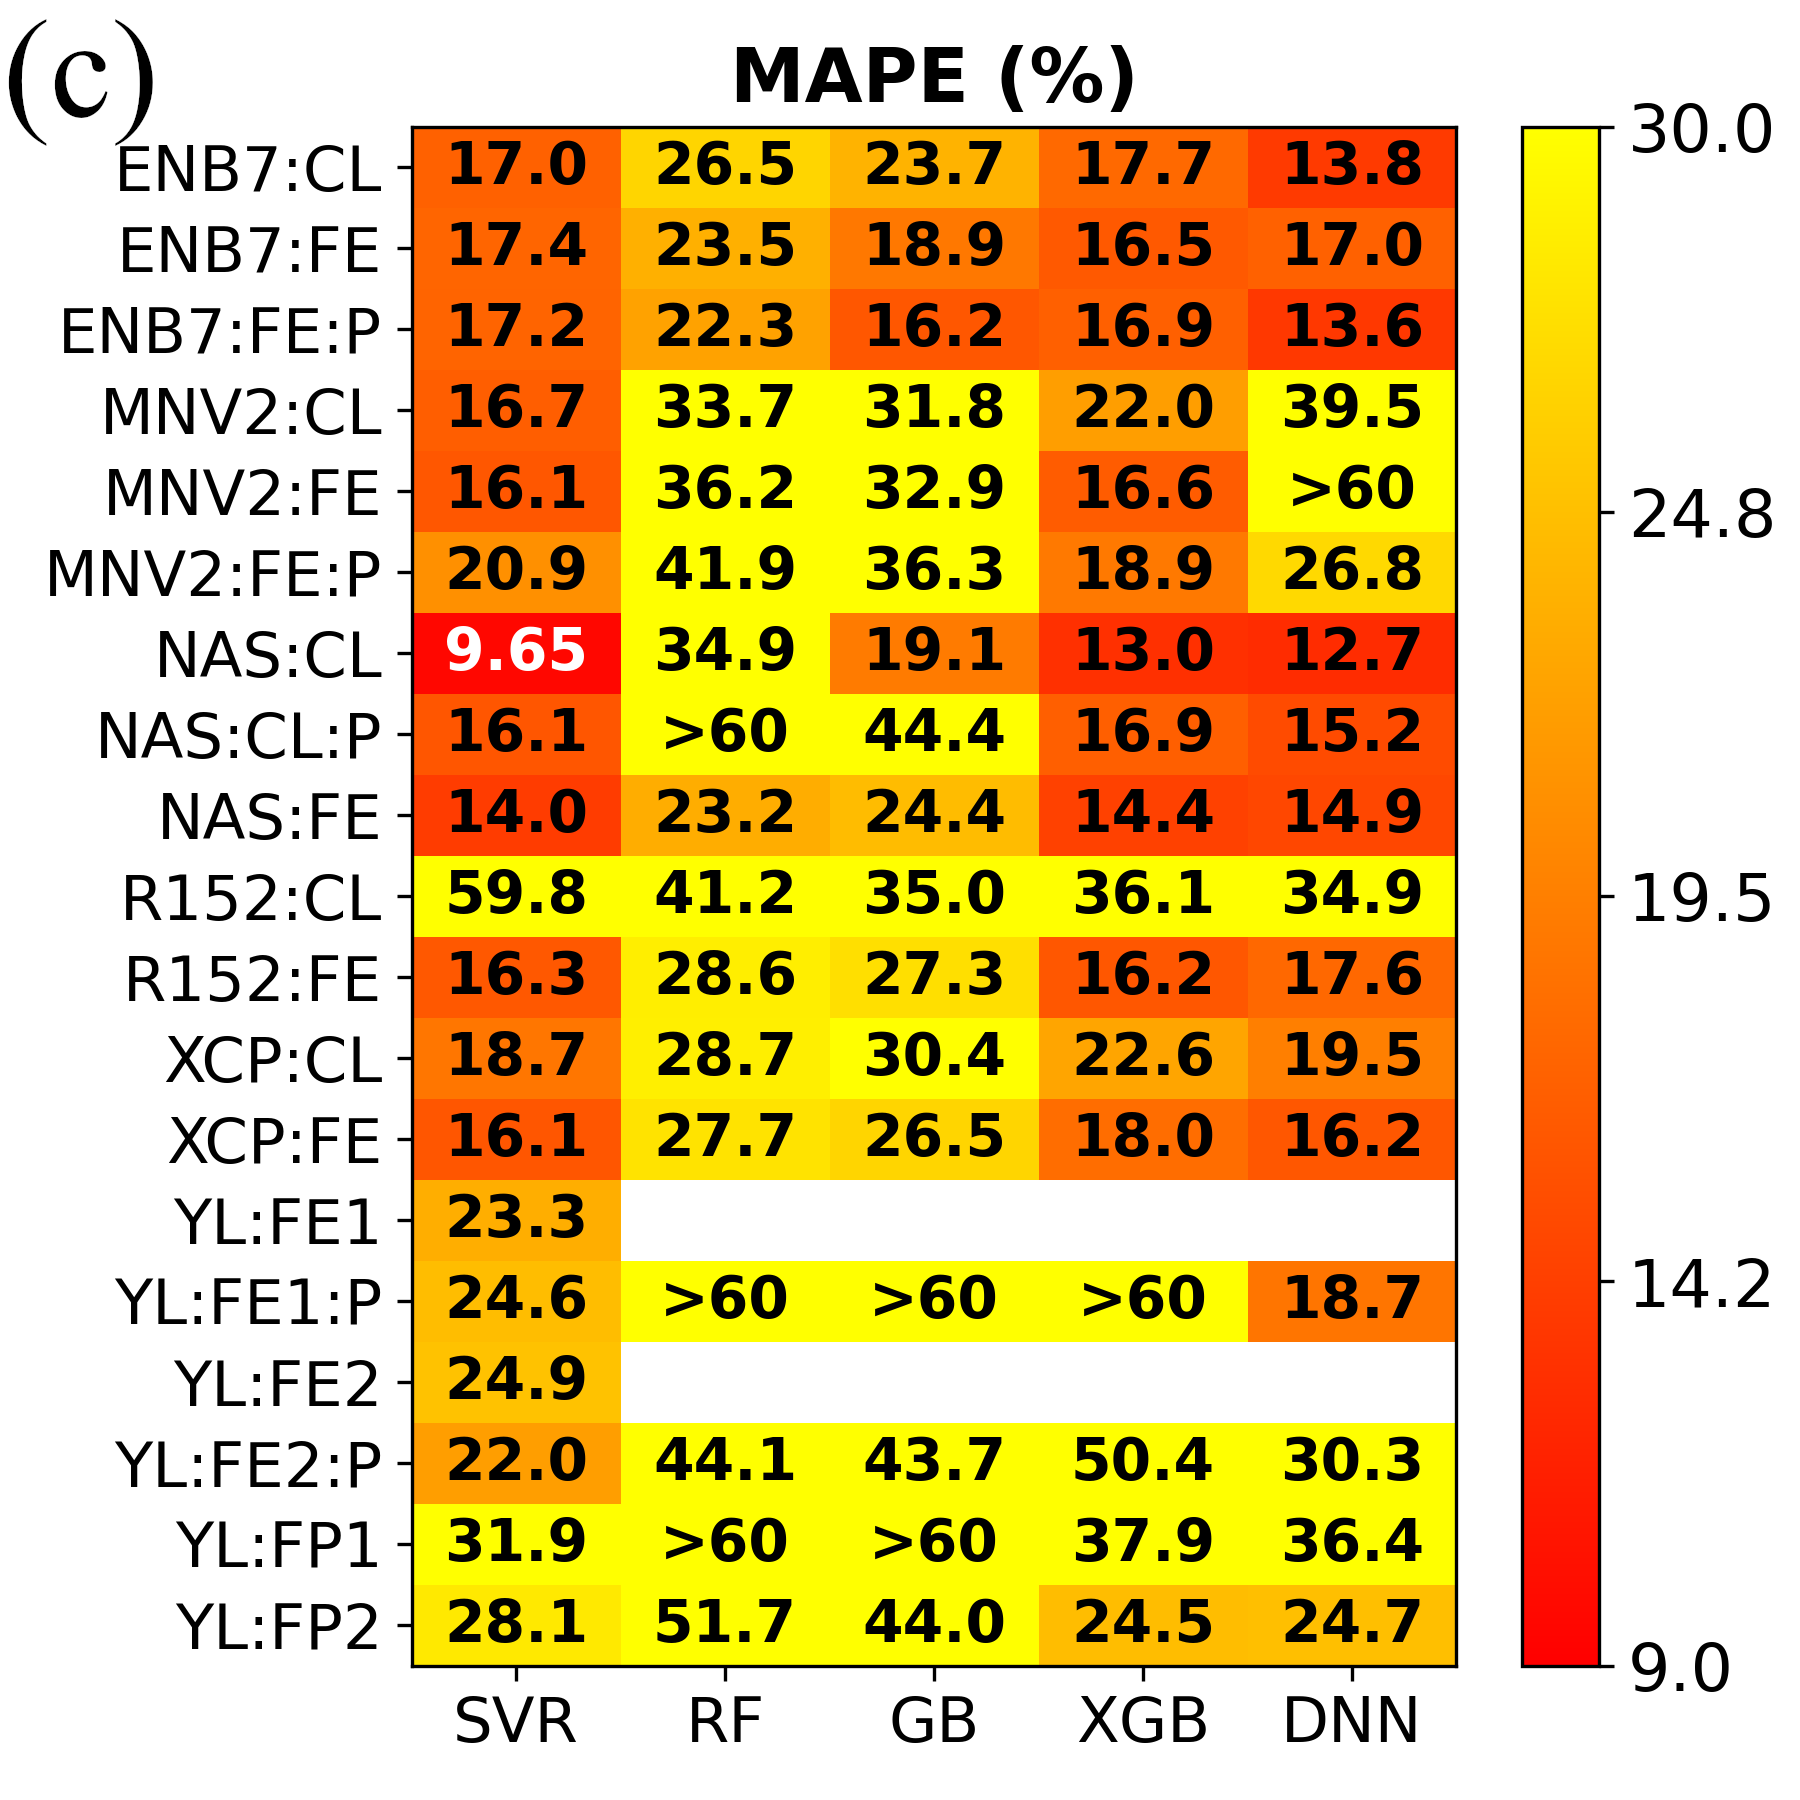
\includegraphics[width=0.35\textwidth]{Fig7c}
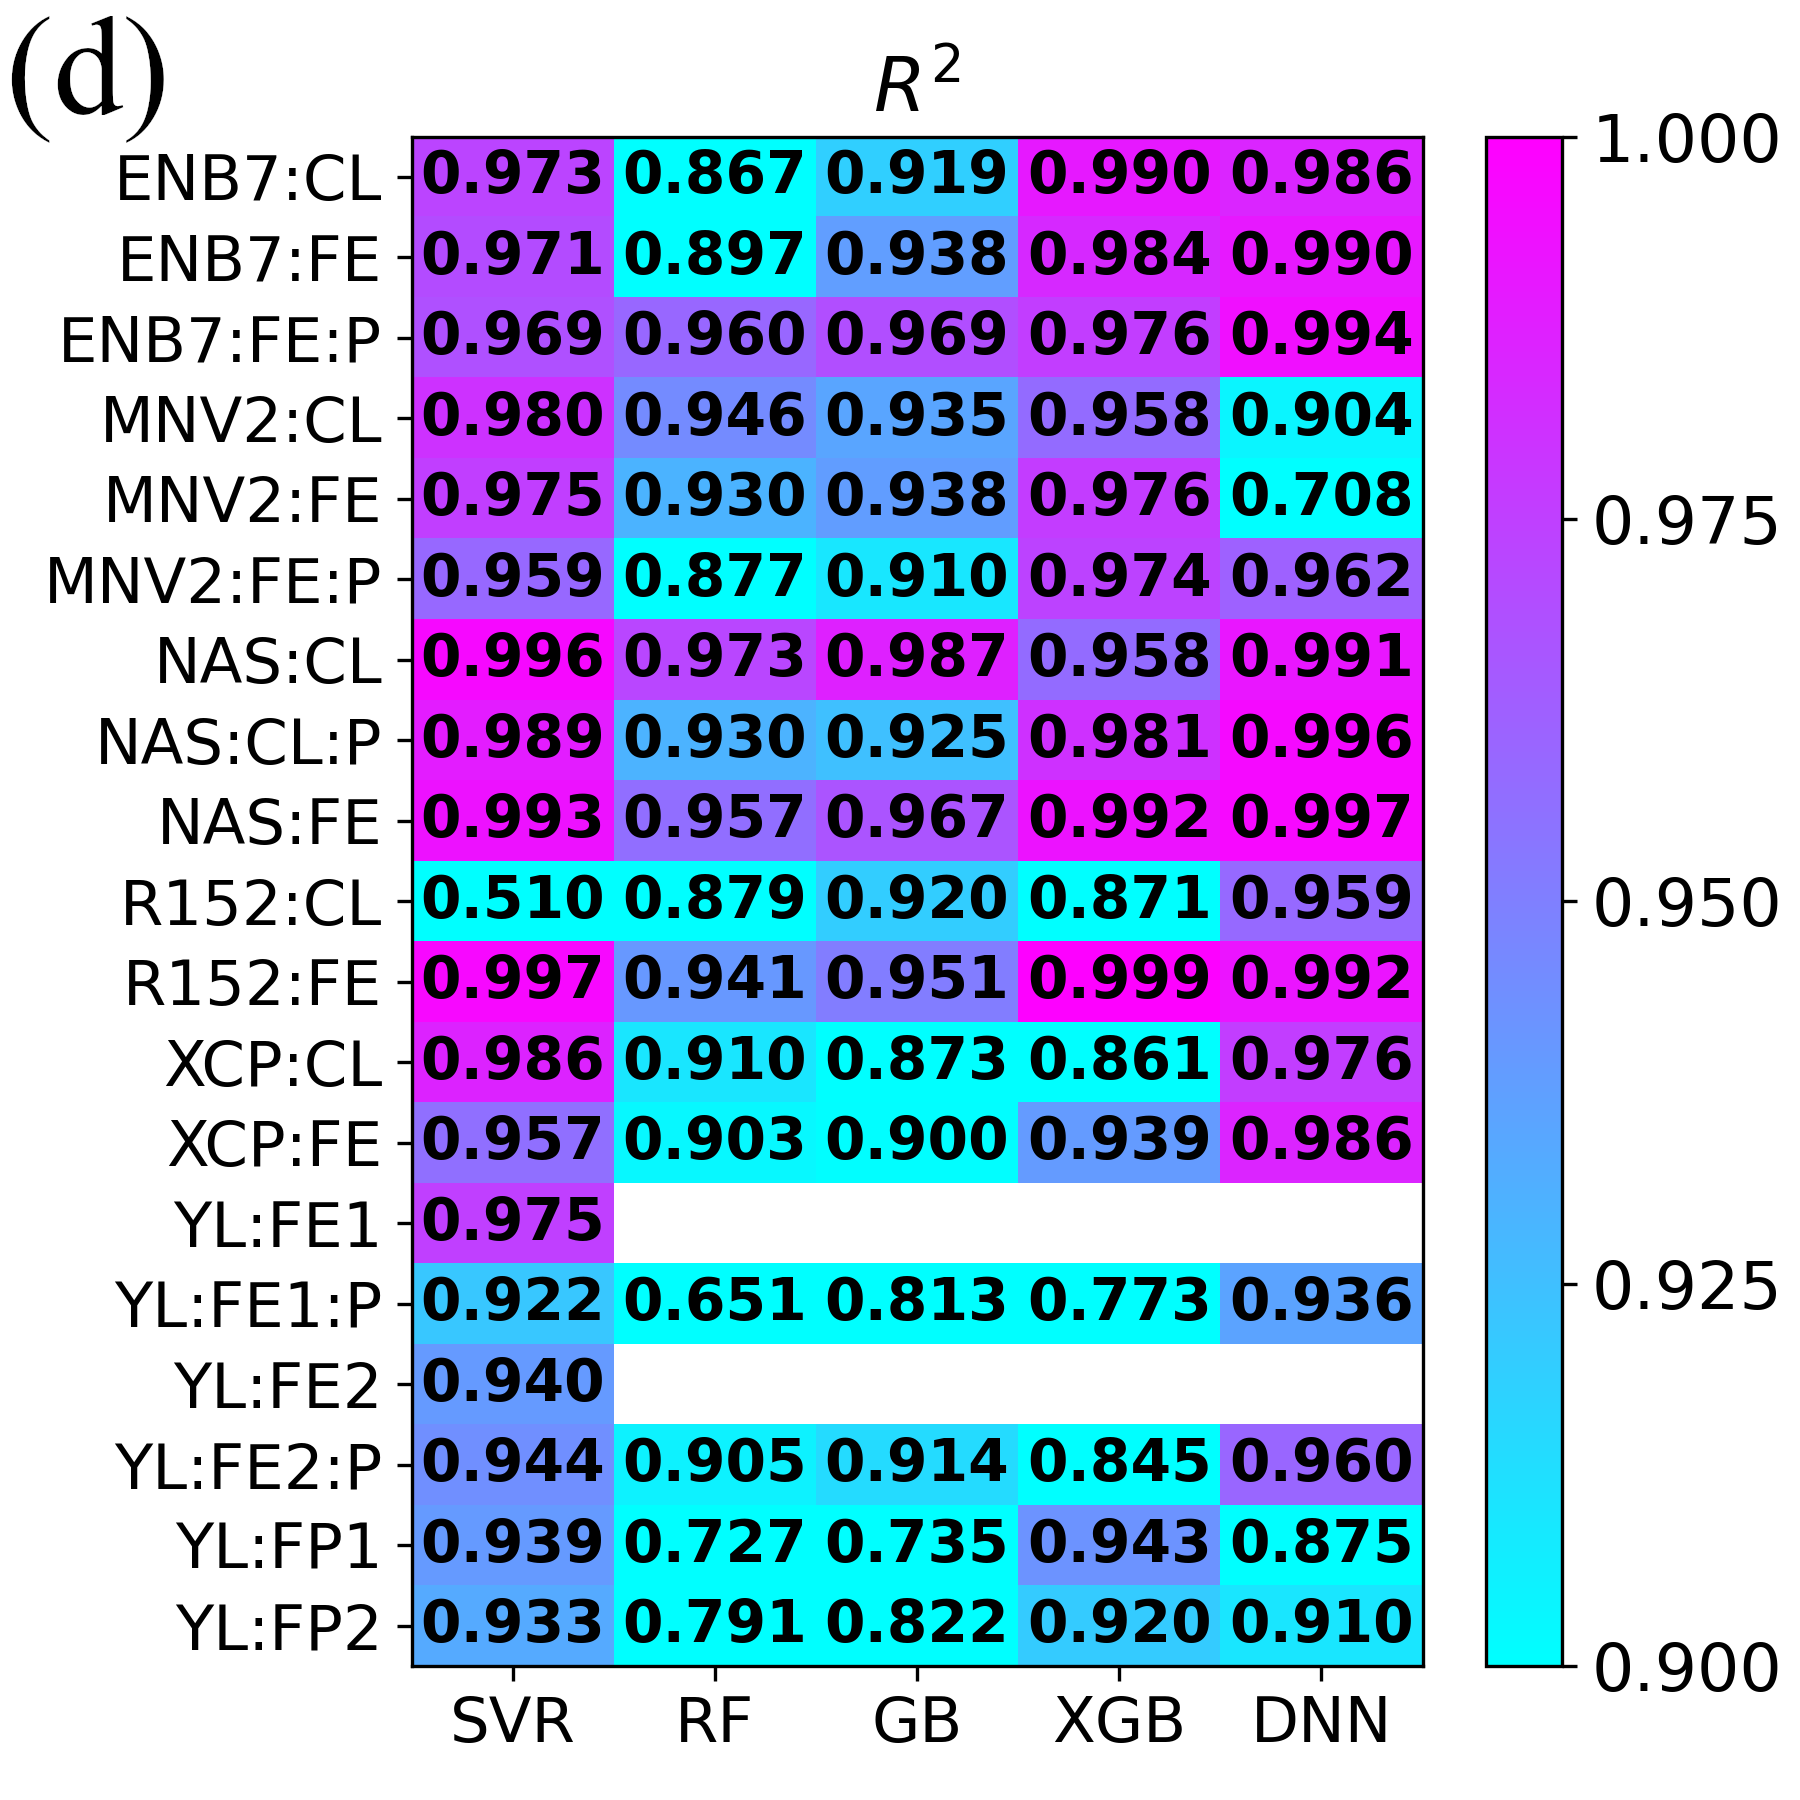
\includegraphics[width=0.35\textwidth]{Fig7d}
\caption{
Mean absolute percentage error (a,c) and coefficient of determination (b, d) for different combinations of CV models (vertical axis)
and regression models (horizontal axis) during the test phase with experimental dataset without (a, b) and with (c, d)
post-hoc calibration according to Eq.~\eref{eqPostHoc}.
The models were trained on a simulated dataset.
}\label{Fig7}
\end{figure*}

While the presence of residual noise patterns in the experimental curves ---
insufficiently suppressed by filtering --- could contribute to the observed discrepancies,
a more plausible explanation lies in the incomplete correspondence between the physical model used for data synthesis and the actual behavior of solar cells.
This mismatch is likely associated with the numerical parameters employed in the model’s fundamental equations (Eqs.~\eref{eqNFet}-\eref{eqTass}).
For instance, the calculation of the characteristic FeB association time (Eq.~\eref{eqTass}) adopted values of
$A=5.7\times10^5\,\frac{\mathrm{s}}{\mathrm{K}\;\mathrm{cm}^3}$ and $E_m=0.66$~eV, which are among the most frequently reported in the literature.
However, a considerable scatter exists in these parameters.
Specifically, $E_m$ values ranging from 0.55~eV \cite{Lauer2016} to 0.69~eV \cite{FeBStrongIll} have been reported,
including intermediate estimates of 0.64 eV \cite{Zhu2011}, 0.65~eV \cite{KimerlingFeB},
0.66~eV \cite{FeBAssSST2011, Le2024, FeBKin2019, FeBJAP2005},
0.67~eV \cite{Zhu2015}, and 0.68~eV \cite{Wijaranakula, Macdonald2004, Zoth1990}.
Similarly, the pre-exponential factor $A$ has been cited as $4.3\times10^5$ \cite{FeBLight2} or $5\times10^5$ \cite{FeBJAP2005, FeBkinAPL2008}.
Moreover, the calculations assumed a spatially invariant $E_m$ across the device.
In practice, the reported diffusion barriers are typically derived for bulk $p$-Si,
whereas the energy value can vary in regions with different Fermi level positions \cite{Murphy2014}, such as the space-charge region in the present structures.
Similar variability exists for other key parameters.
The FeB pair binding energy has been reported to range from 0.45 to 0.67~eV \cite{KimerlingFeB, Zhu2015, Wijaranakula, Hayamizu1991},
the Fe$_i$ donor level position varies between 0.38 and 0.394~eV above the valence band maximum \cite{FeBAssJAP2014, Macdonald2004, FeB:Schmidt, Narland},
and the pre-exponential factor in denominator of Eq.~\eref{eqFeieq} $A_z$ has been cited as either
$10^{-23}$~cm$^{3}$ or $2.7\times10^{-22}$~cm$^{-3}$~cm$^{3}$ \cite{Zhu2015}.
A deviation of any of these parameter values from their actual physical magnitudes could account for the observed prediction errors.
Furthermore, earlier studies have demonstrated that both the non-uniform distribution of iron across the base thickness
and the variation in the base thickness itself can significantly affect iron concentration estimation \cite{KimerlingFeB}.
Neither of these effects was incorporated into the present modeling framework.

A common strategy to improve prediction accuracy involves post-hoc calibration,
where a corrective function is applied to model outputs using parameters derived from a limited subset of experimental data.
In the present case, the analysis indicated that a quadratic correction of the target variable provides
the most suitable adjustment, expressed as follows:
\begin{equation}\label{eqPostHoc}
  \log N_\mathtt{Fe,PRED}=9.51-1.71\cdot \log N_\mathtt{Fe,PRED}^{*} + 0.079 \cdot (\log N_\mathtt{Fe,PRED}^{*})^2\,,
\end{equation}
where $N_\mathtt{Fe,PRED}^{*}$ denotes the direct model prediction.
The performance metrics after post-hoc calibration are presented in \Fref{Fig7}c and \Fref{Fig7}d.
As shown by the data, applying this correction substantially reduced the prediction errors.
Specifically, the mean relative error across the 28-sample experimental dataset now lies within the (13–17)\% range
for the best-performing models (approximately 20 out of 87 configurations) and remains below 25\% for most of the others.
The median error is even lower, reaching (7–10)\% in the most favorable cases.
In line with the results obtained for the simulated test dataset, the most accurate configurations involve EfficientNetB7, NASNetLarge, DNN, SVR, and XGB.
Interestingly, MobileNetV2 also appeared among the top-performing combinations, yielding the lowest MedAPE value (7.64\%) for the MNV2:CL configuration.
This outcome may suggest that the features extracted by MobileNetV2, though less informative for the training and simulated test datasets,
capture specific image patterns more relevant to the experimental measurements and applied correction could have further enhanced the effectiveness of these features.

It is worth noting that applying the correction increased the gap between the mean and median absolute percentage errors.
This observation suggests that, although the correction improved the overall agreement between the predicted and true values,
a few samples still exhibit relatively large residual errors.

The correction also led to a decrease in the $R^2$ value.
This outcome is expected, as post-processing can weaken the linear correspondence between the initial predictions and the experimental values,
even when the overall prediction errors are simultaneously reduced.
Therefore, the reduction in $R^2$ should be regarded as a side effect of enhancing
the model’s accuracy rather than as evidence of its degradation.

Although the quadratic correction proved effective, it does not represent a universal solution
for transferring models from synthetic to experimental data.
 A more robust approach involves integrating experimental data into the training process, as implemented in this study below.



\subsection{Experimental data}

\Fref{Fig8} shows the correlation between the iron concentrations predicted by models trained on experimental data
and reference values derived according to \cite{Olikh2022:JMatSci,Olikh2021JAP}.
Representative outcomes for selected CV–regression model combinations are shown for both training and testing,
with extended data provided in Figure~S6 of the Supplementary Material.


\begin{figure*}
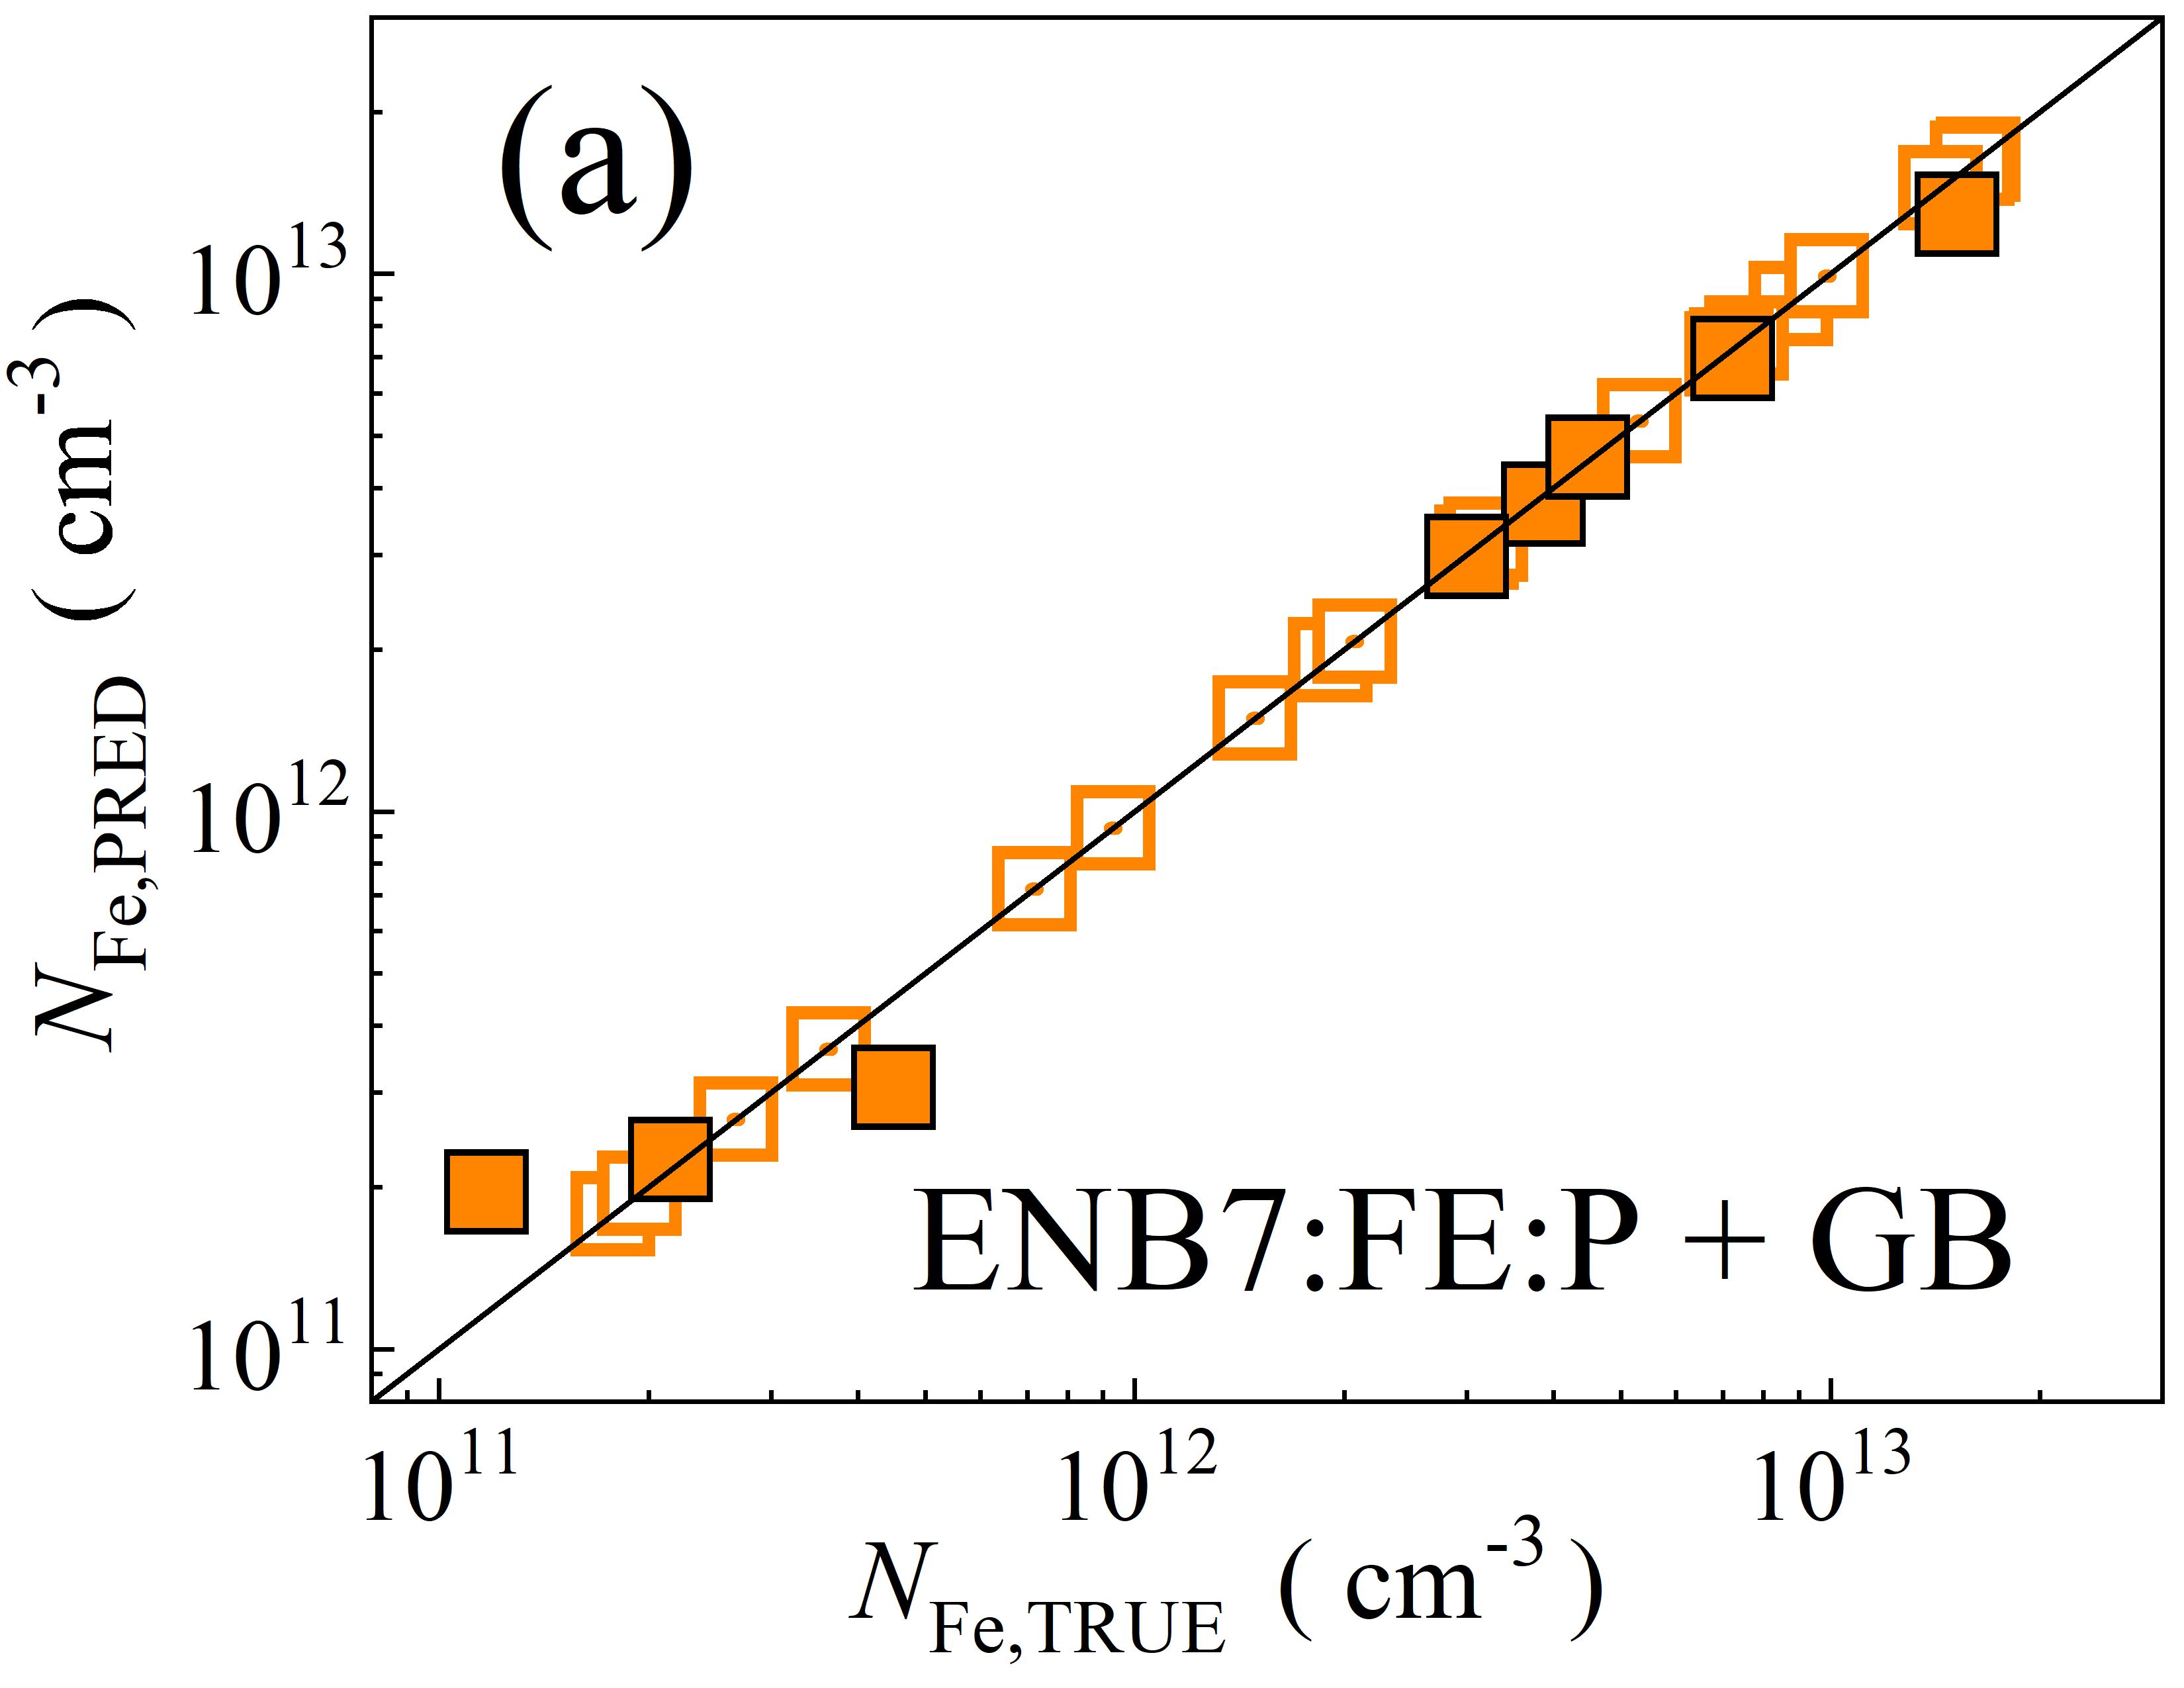
\includegraphics[width=0.33\textwidth]{Fig8a}
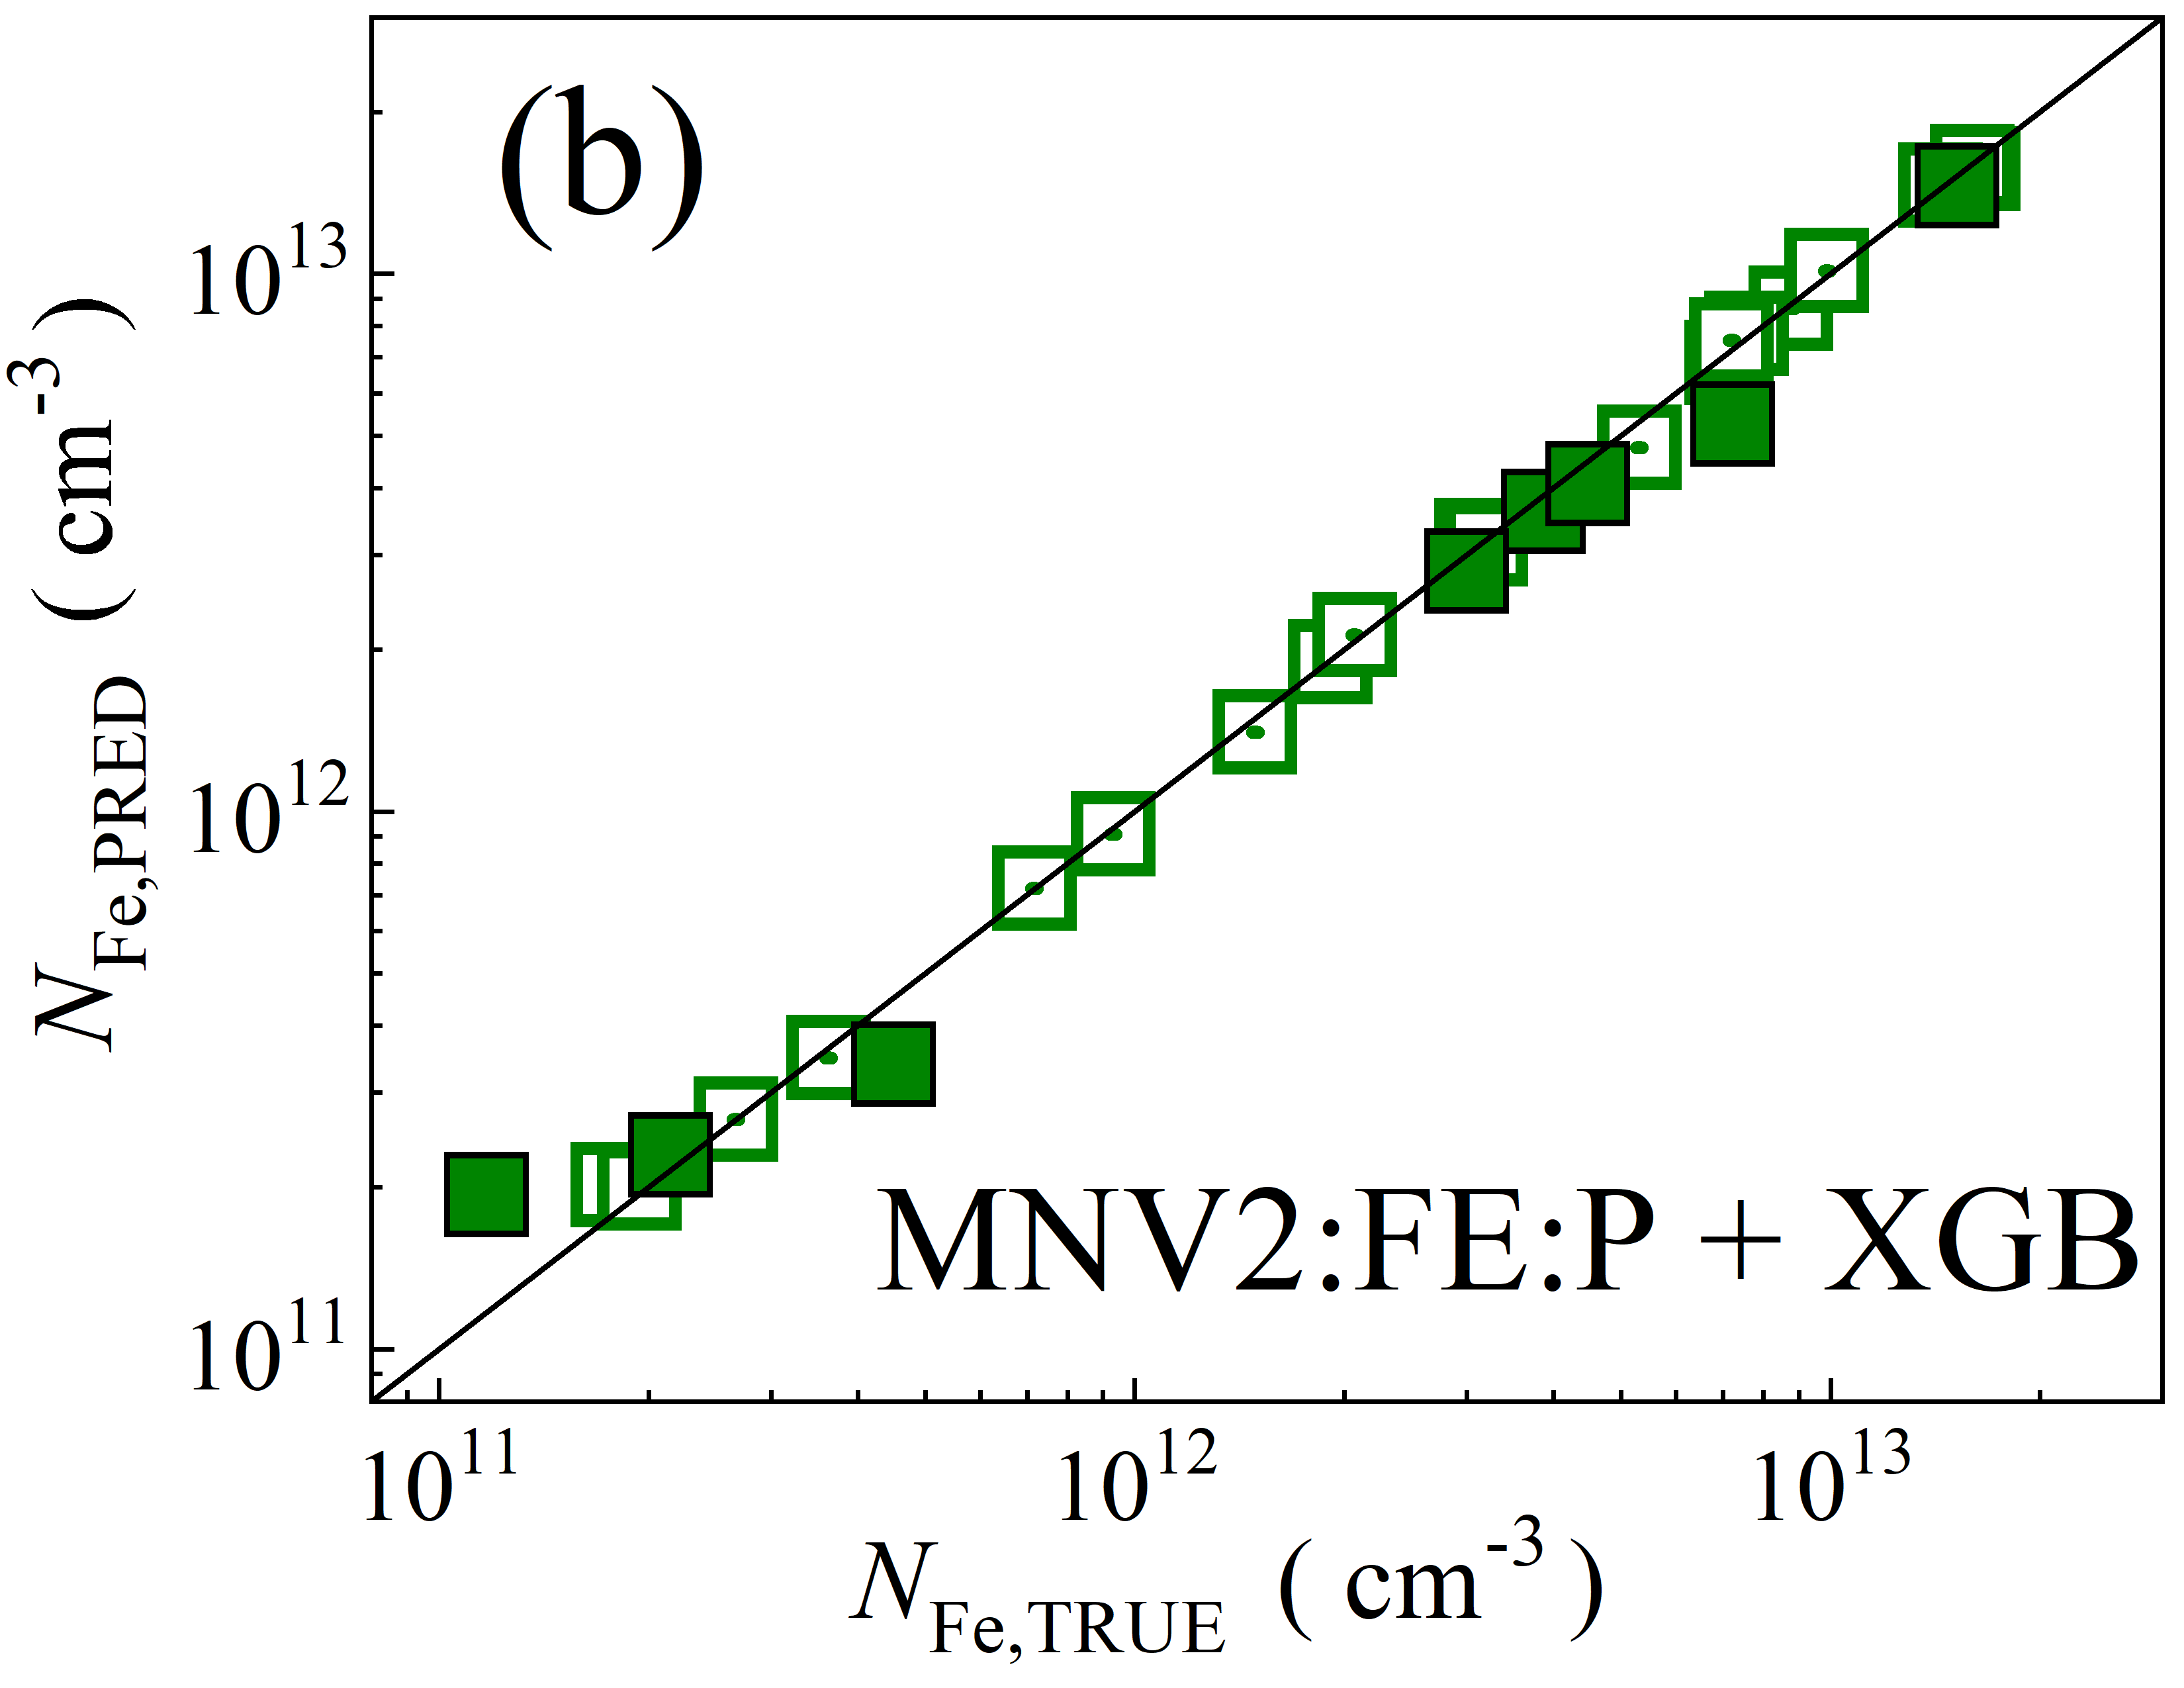
\includegraphics[width=0.33\textwidth]{Fig8b}

\includegraphics[width=0.33\textwidth]{Fig8c}
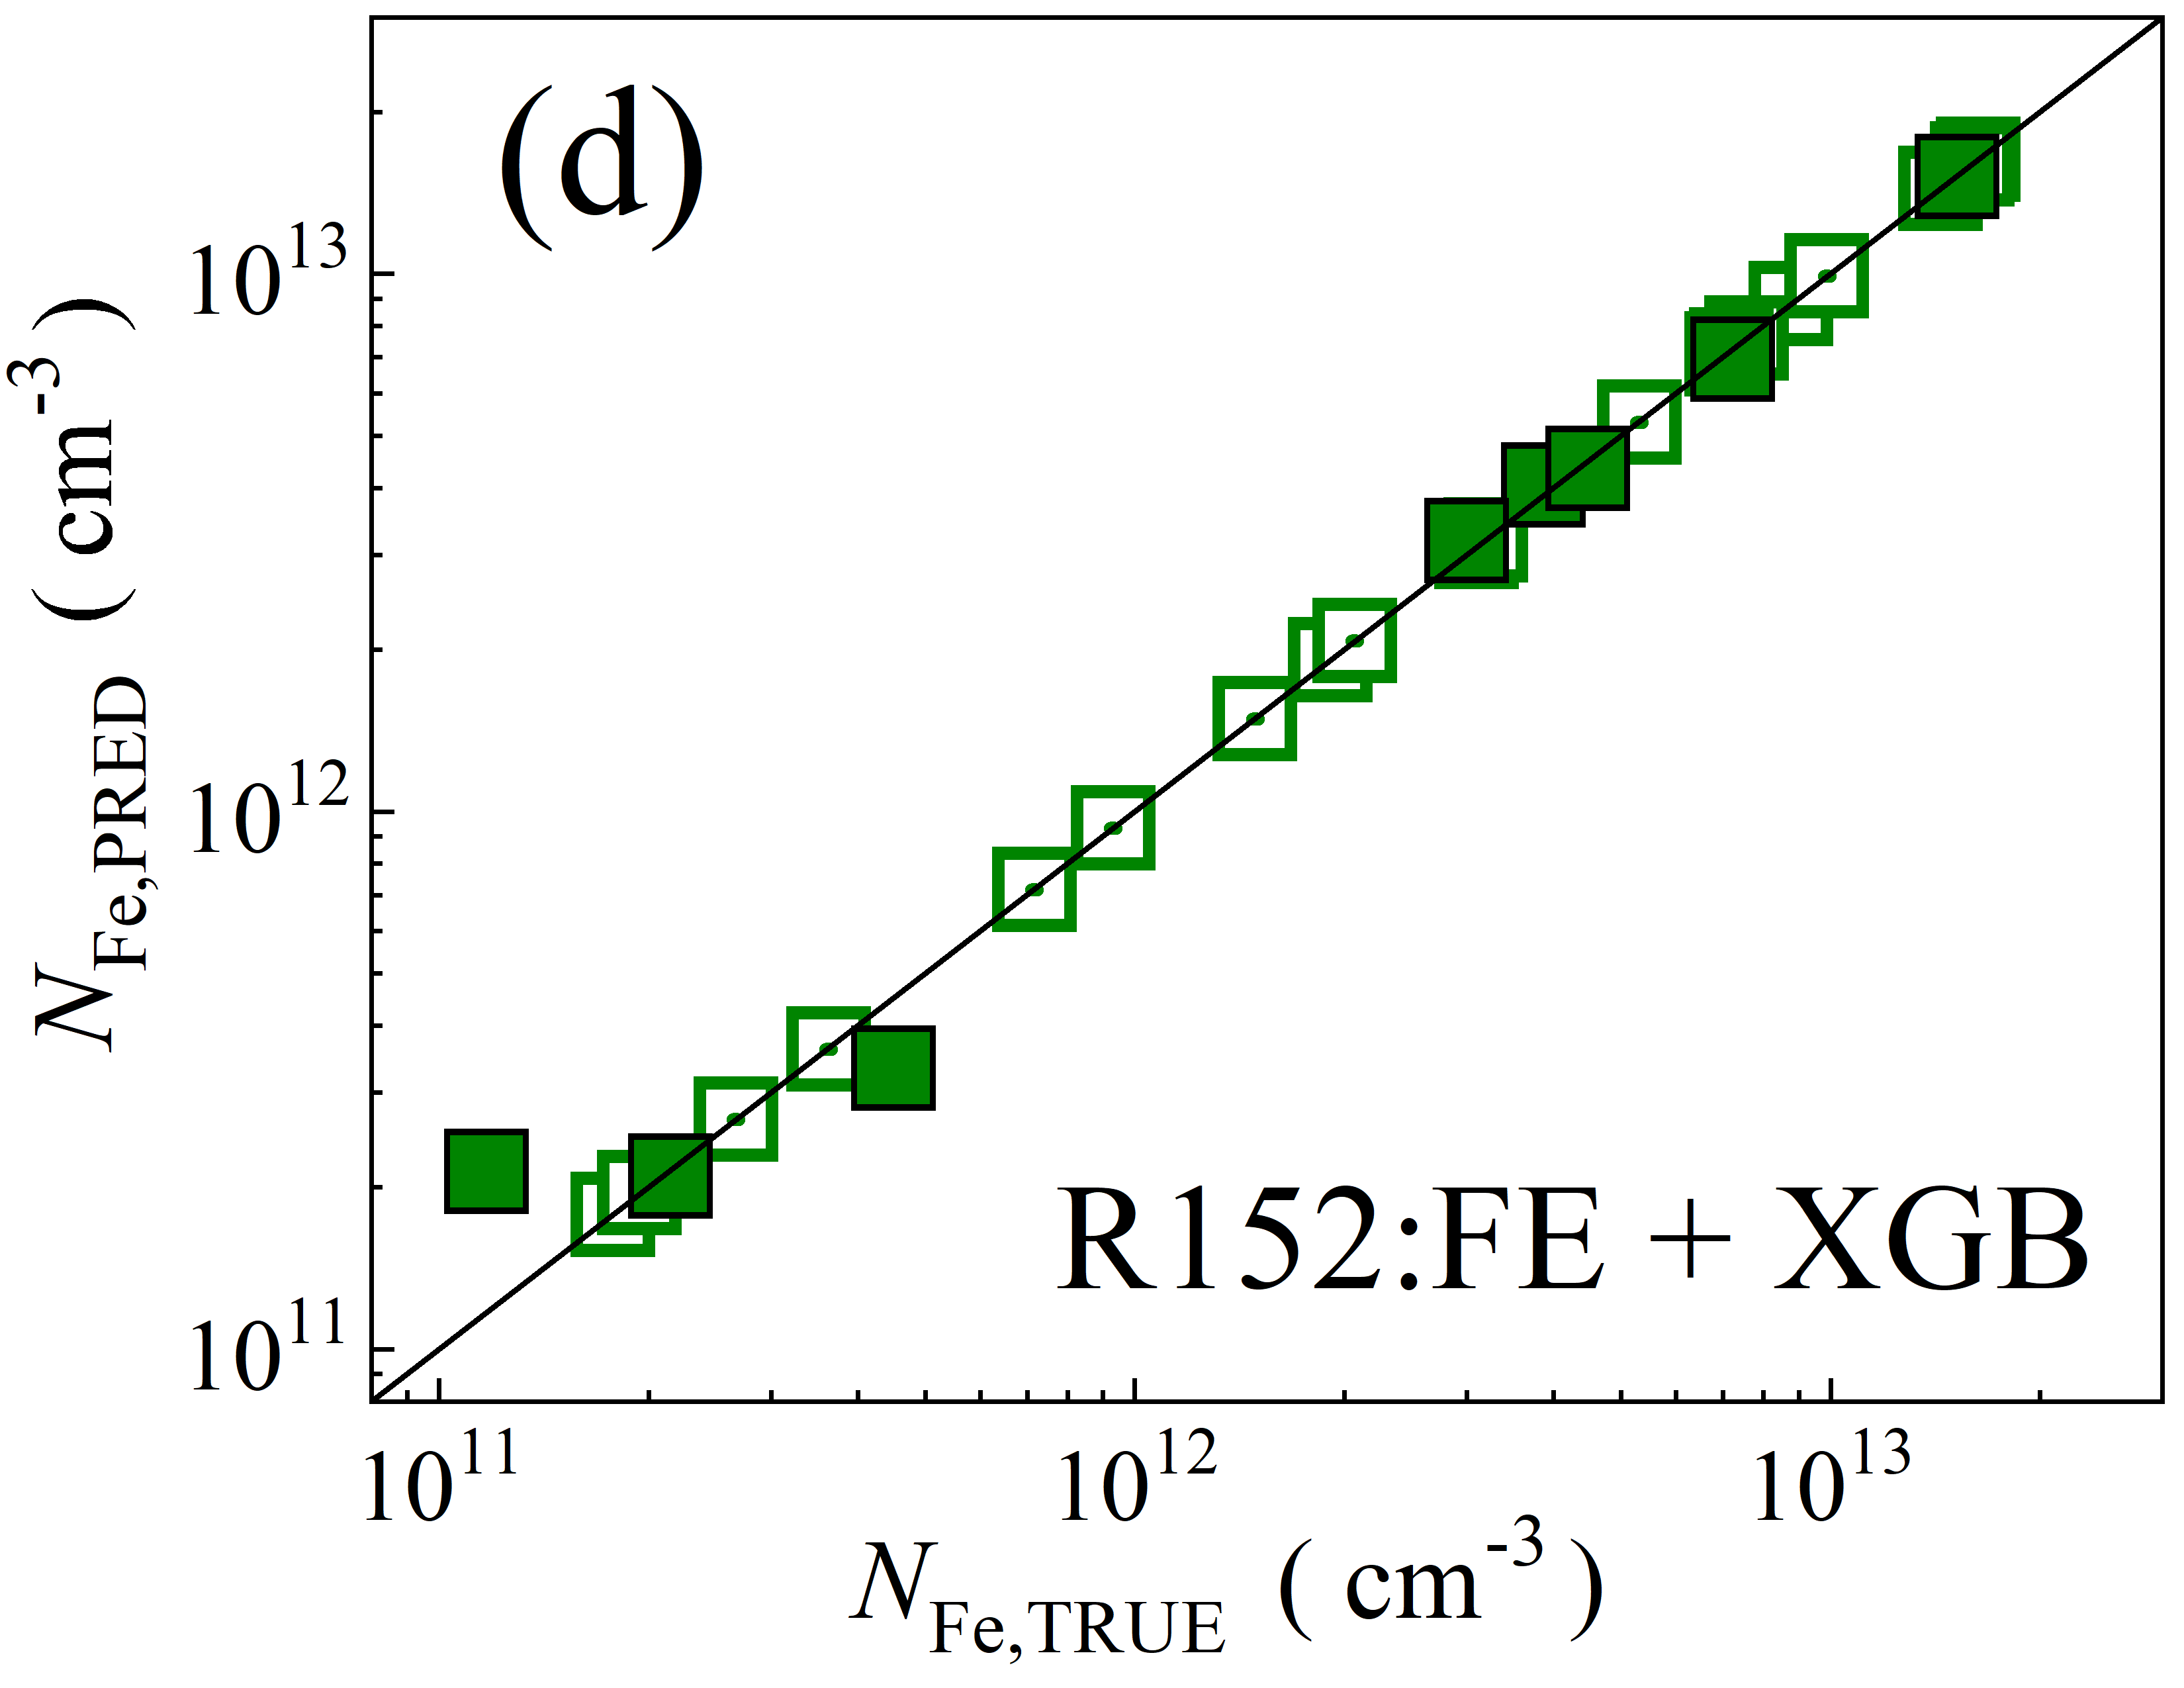
\includegraphics[width=0.33\textwidth]{Fig8d}
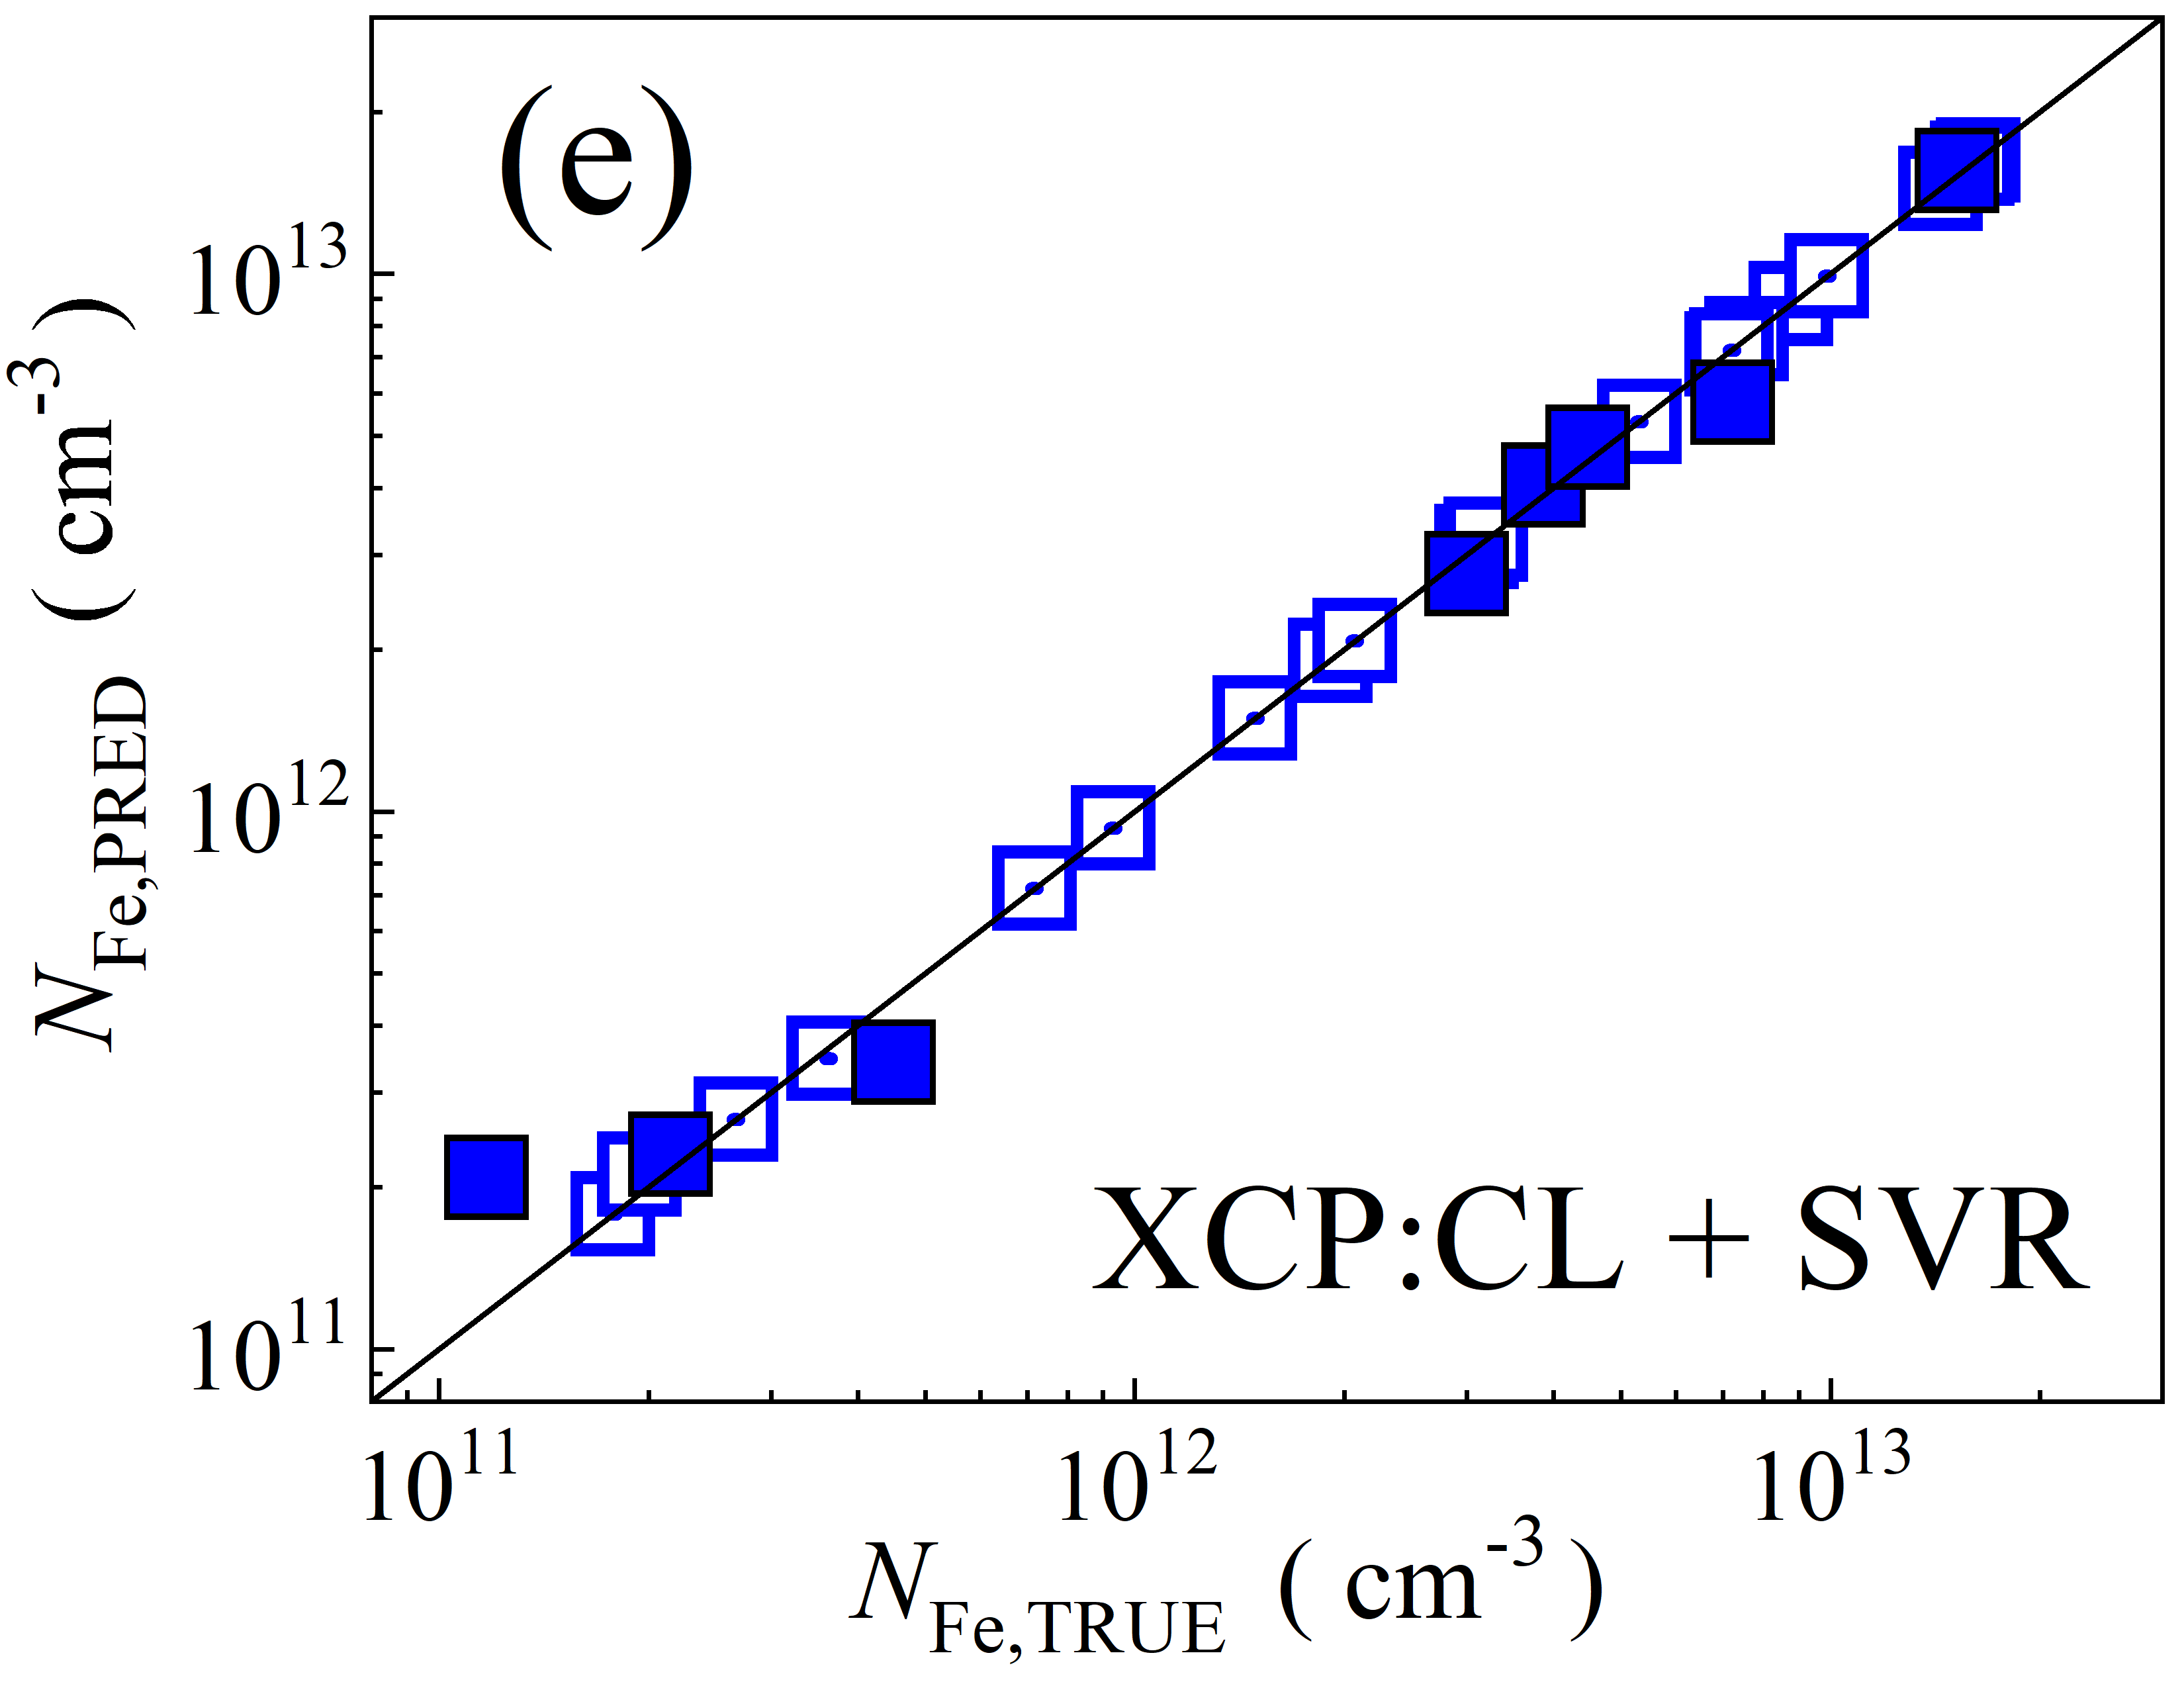
\includegraphics[width=0.33\textwidth]{Fig8e}
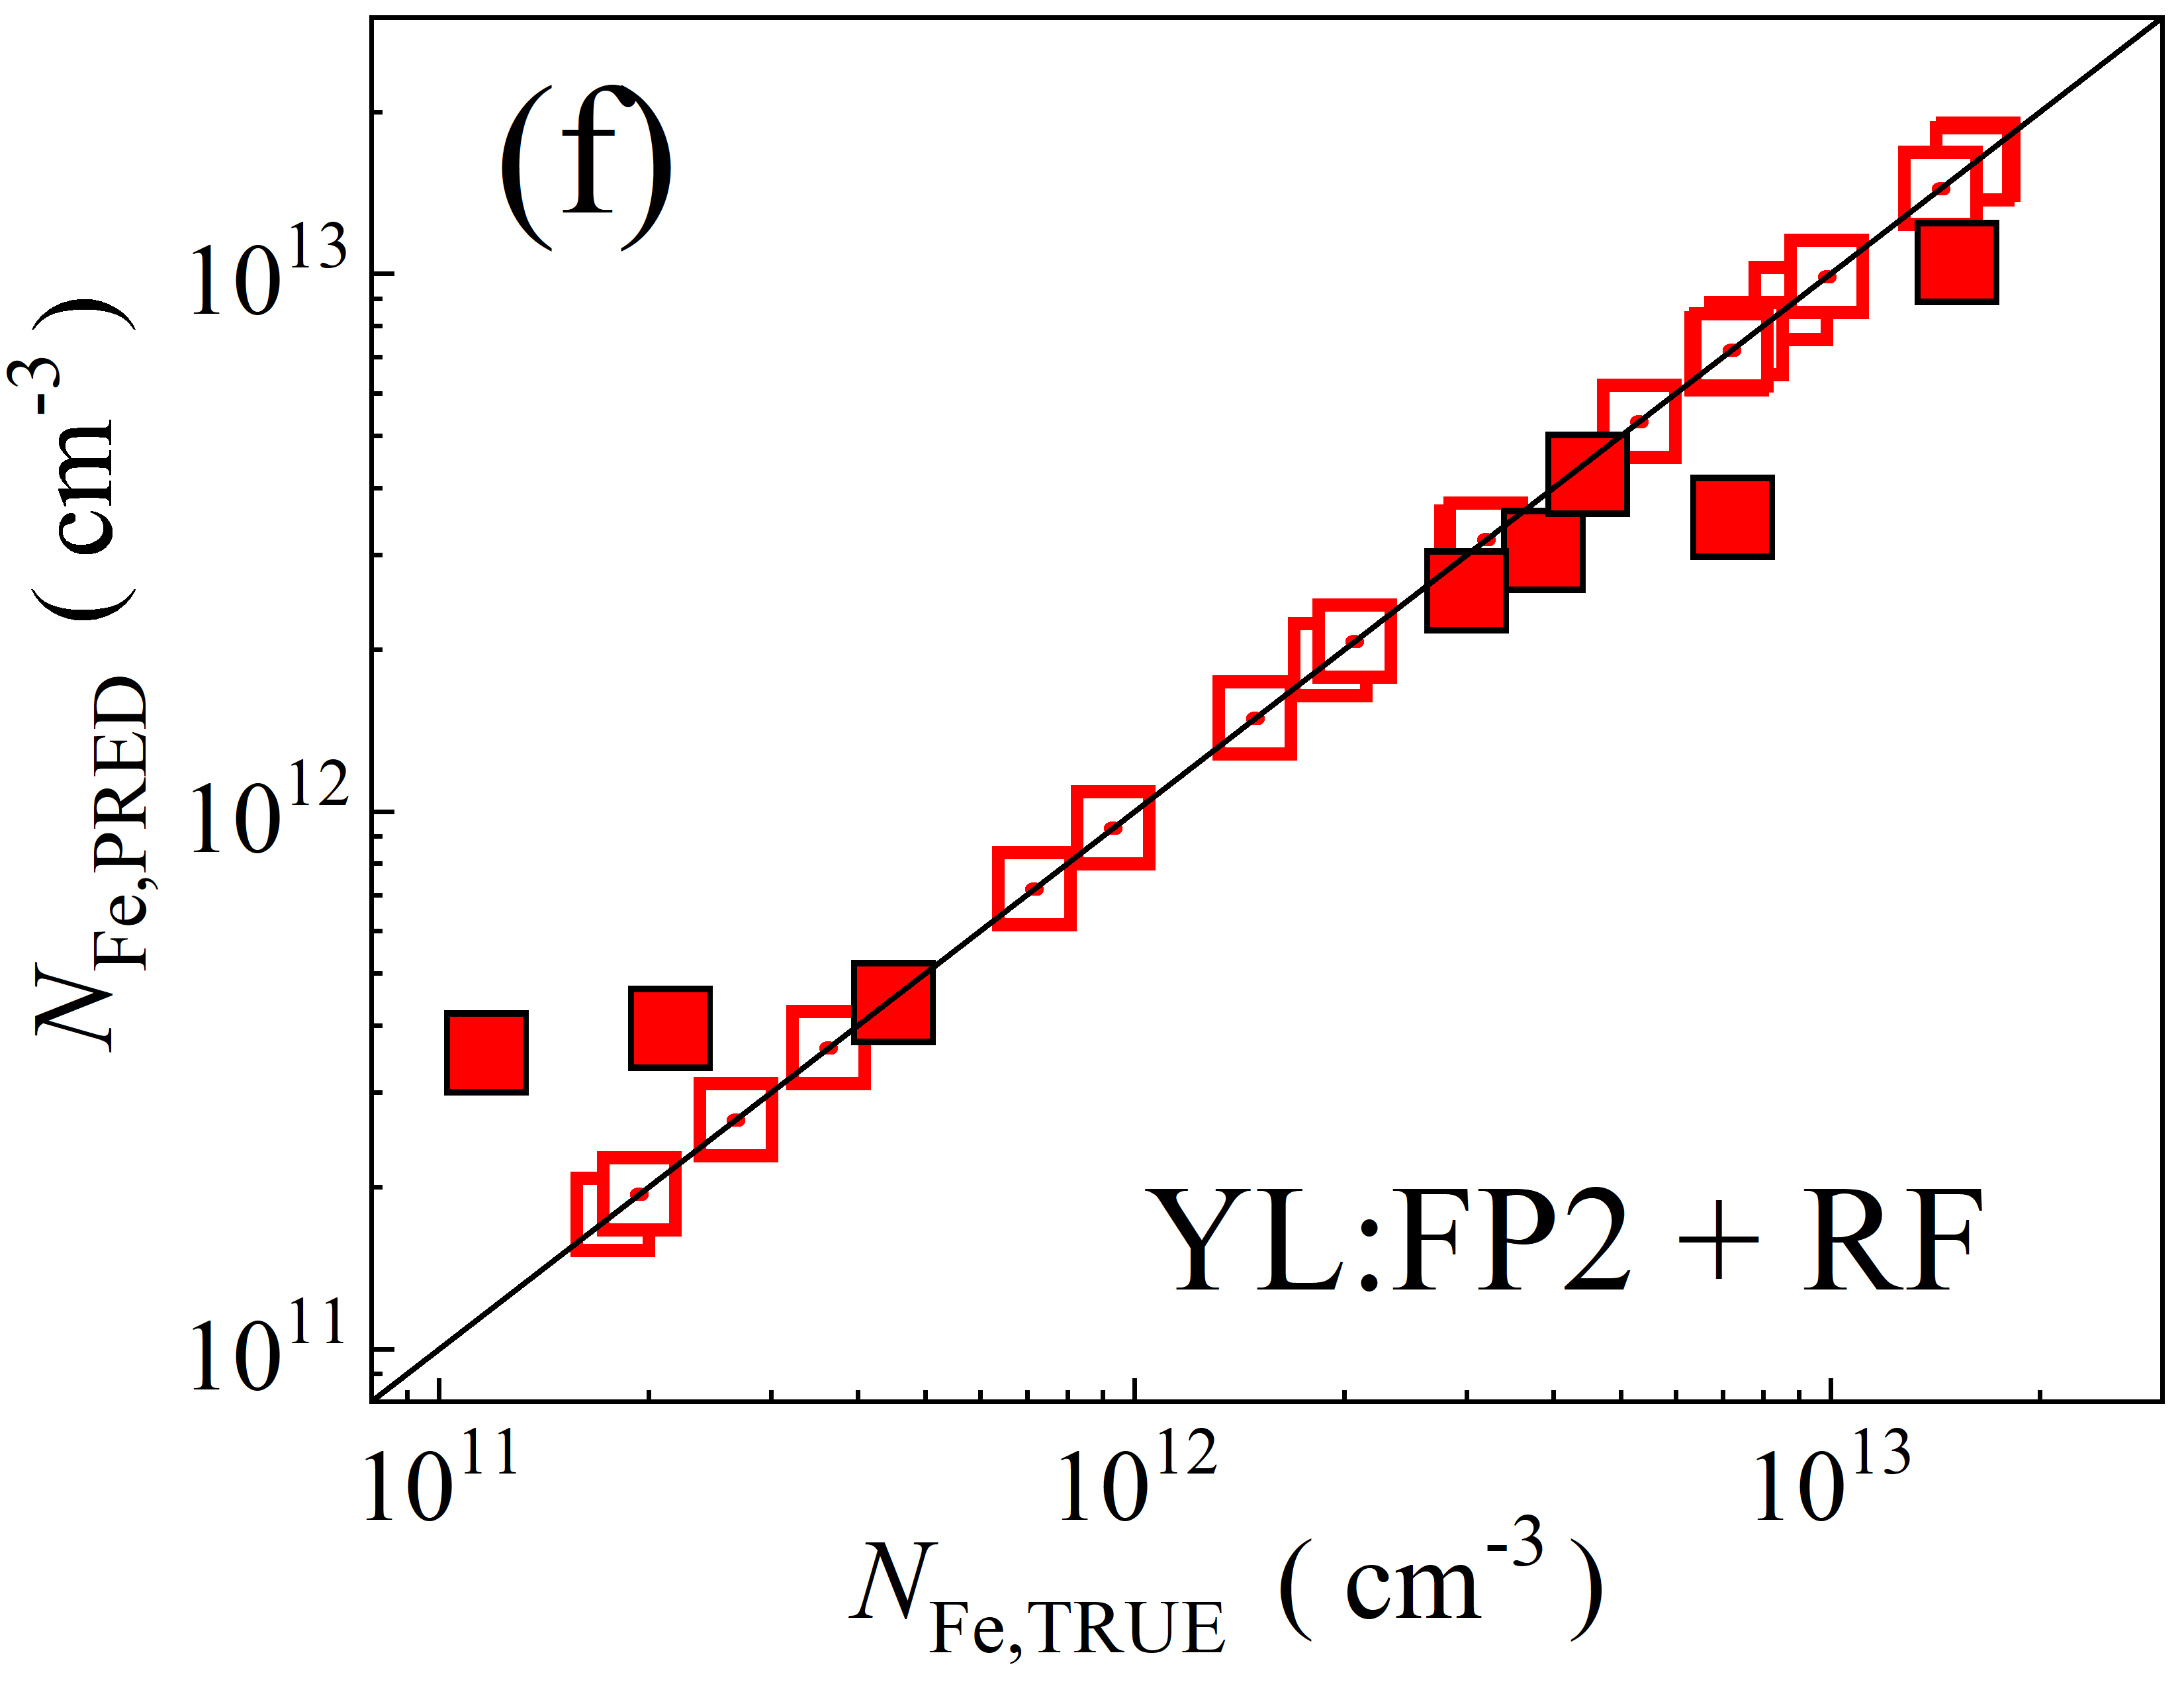
\includegraphics[width=0.33\textwidth]{Fig8f}
\caption{
Scatter plots compare the reference iron concentrations $N_\mathrm{Fe,TRUE}$ with ML-predicted values $N_\mathrm{Fe,PRED}$,
obtained using feature vectors extracted from various CV models combined with different regression algorithms
(specific models are indicated in the figures).
The ML models were trained on a dataset derived from experimental measurements.
The open and filled squares correspond to the training and test phases, respectively.
The black lines are the identified lines serving as the references.
}\label{Fig8}
\end{figure*}

It should be noted that, compared to training on synthetic data, this case employed an even smaller sample set (20 samples versus 25).
However, these samples covered a narrower range of iron concentrations ($10^{11}$-$2\times10^{13}$~cm$^{-3}$ versus $10^{10}$-$10^{14}$~cm$^{-3}$).
\Fref{Fig9} presents a subset of the performance metrics obtained during the training phase
(a more comprehensive overview is provided in Figure~S7).
Overall, the results are similar to those shown in \Fref{Fig5}.
In many cases, extremely low errors (below 0.5\%) and high coefficients of determination (approaching unity) were observed.
This behavior is particularly characteristic of GB, RF, and SVR.
As in the previous case, the DNN exhibited weaker performance relative to the other algorithms,
although its results slightly improved compared to those for the simulated training dataset.
This improvement may stem from the greater homogeneity of the experimental data.
The leading performance of EfficientNetB7 and NASNetLarge among the CV models was again confirmed,
indicating that these architectures produce the most relevant features for this task.
However, the performance gap relative to other CV models has become less pronounced.

\begin{figure*}
\centering
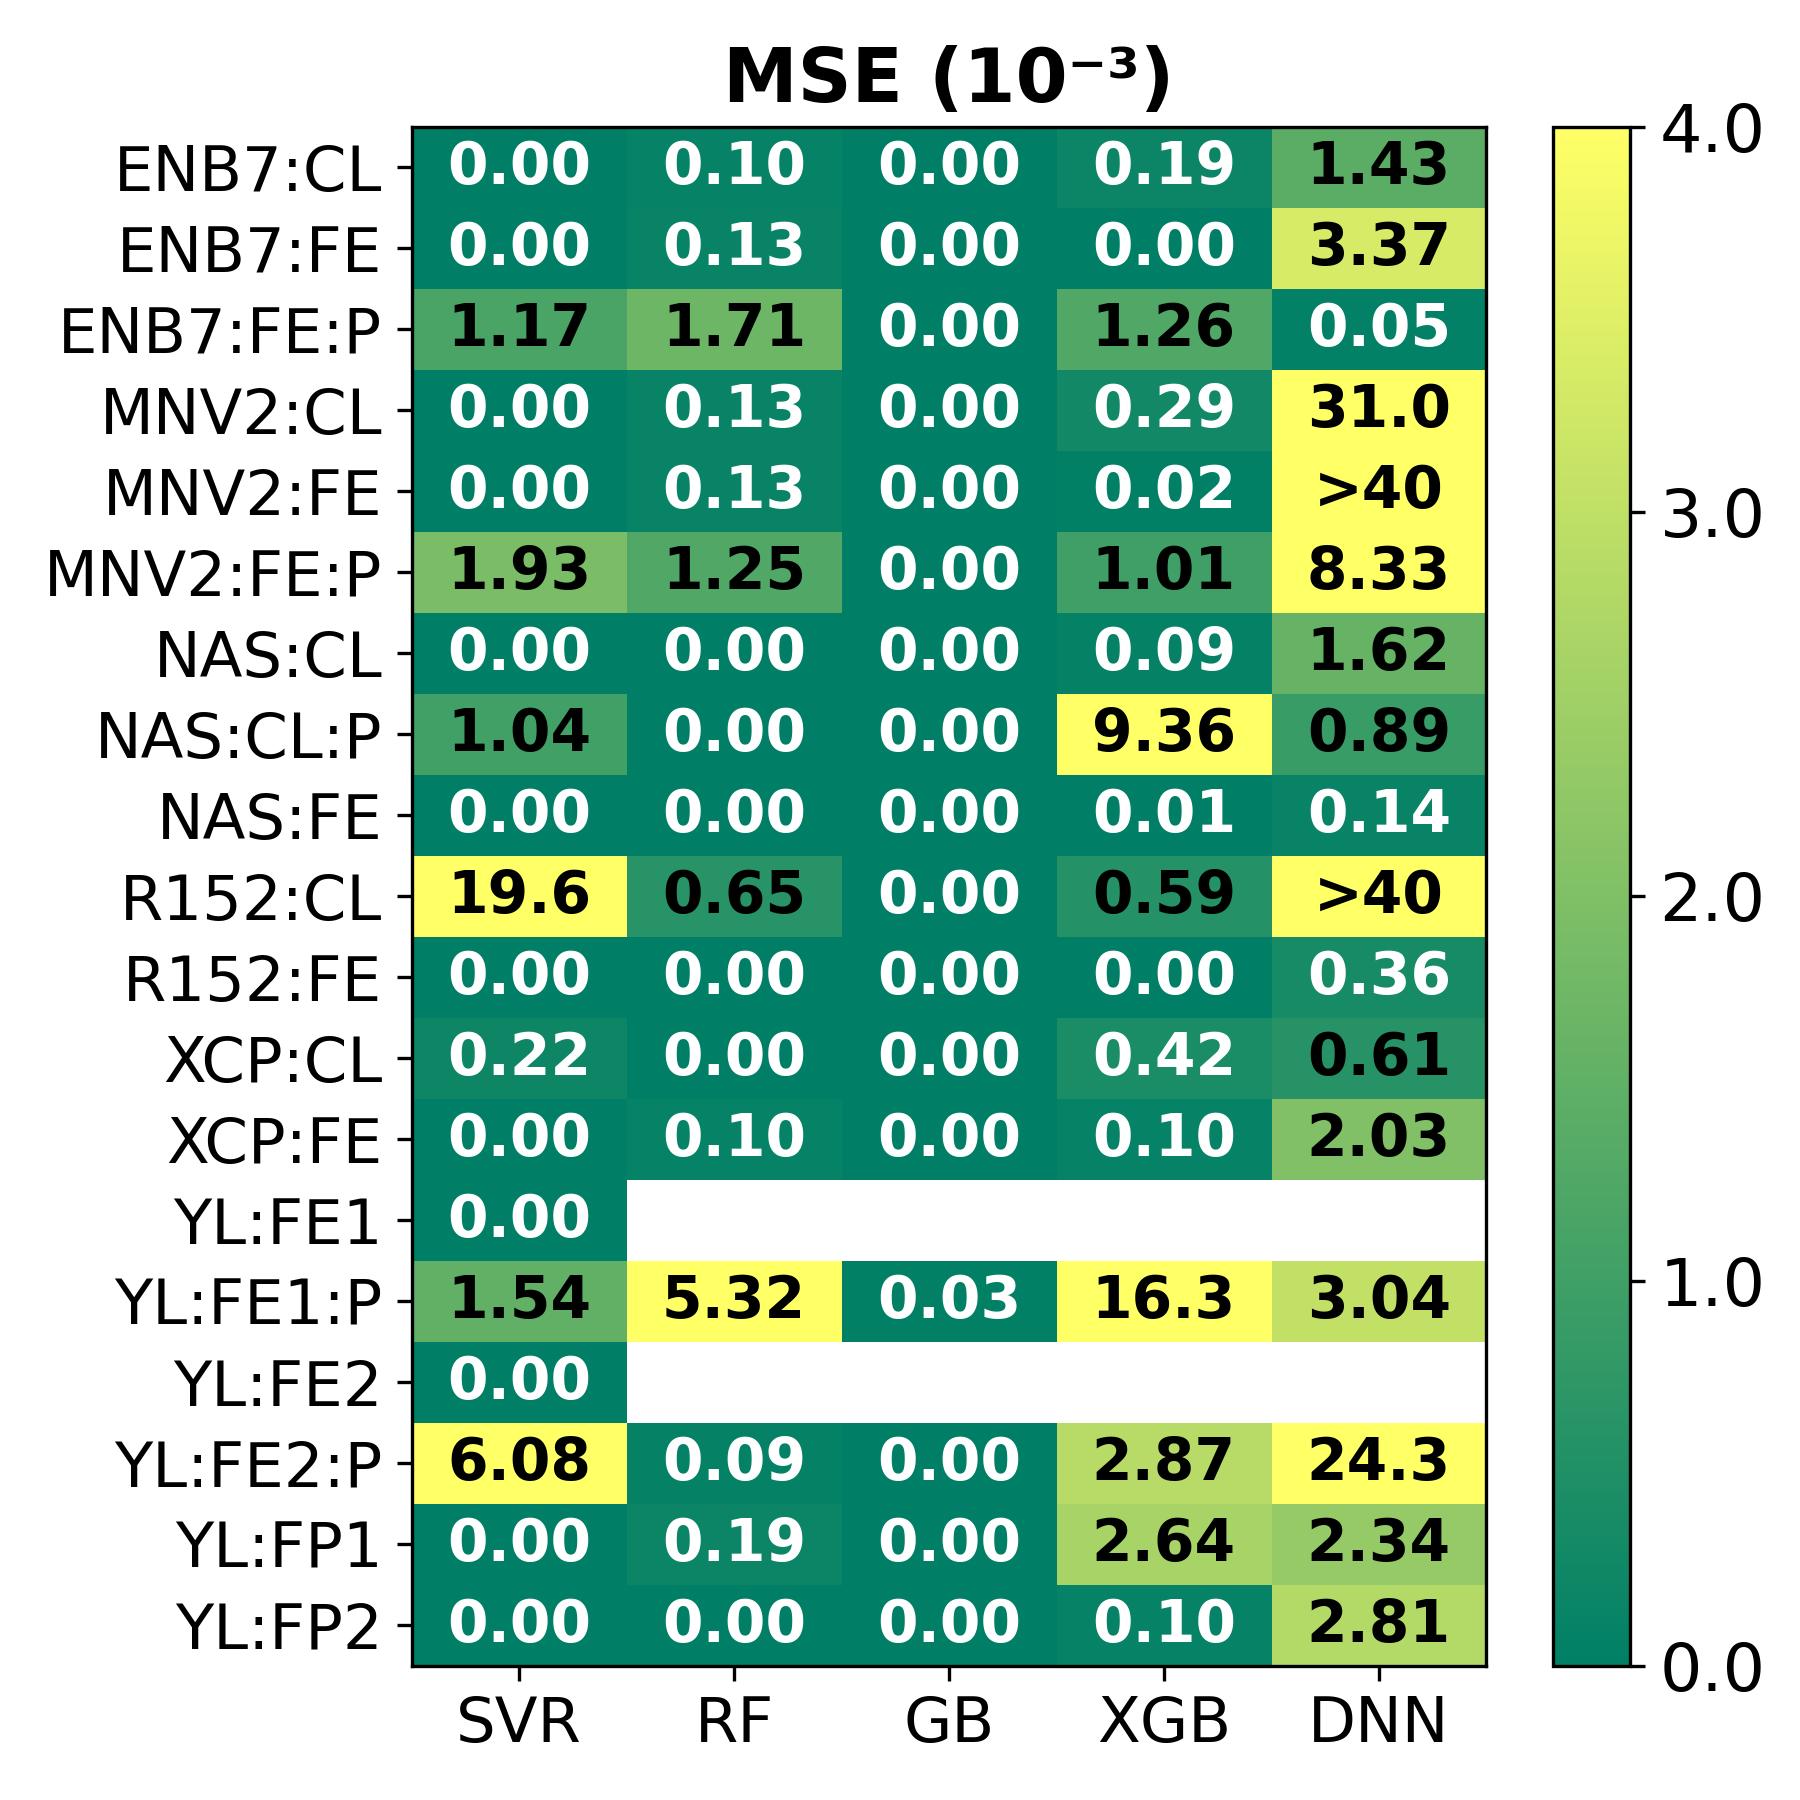
\includegraphics[width=0.35\textwidth]{Fig9a}

\includegraphics[width=0.35\textwidth]{Fig9b}
\caption{
Mean squared error (left panel) and median absolute percentage error (right model) for different combinations of CV models (vertical axis)
and regression models (horizontal axis) during the training phase.
The models were trained on an experimental dataset.
}\label{Fig9}
\end{figure*}

Interestingly, the application of PCA often enhances the performance of the DNN.
For example, the MAPE values for ENB7:FE and ENB7:FE:P are 7.3\% and 0.97\%, respectively.
This observation suggests that PCA effectively mitigates the adverse effects of high feature dimensionality
when the sample size is limited.
In contrast, a similar improvement is not observed for other regression algorithms.
Moreover, for the experimental training dataset,
the difference between MAPE and MedAPE becomes smaller.
This reduction implies a more symmetric error distribution and a decreased occurrence of extreme deviations.

\Fref{Fig10} and Figure~S8 show the heatmaps of prediction metrics for the test experimental dataset
using models trained on a separate subset of experimental data.
Compared to models trained on simulated data, the predictive performance for experimental test dataset improved substantially.
In particular, for several of tthe best-performing CV–regressor combinations, MAPE and MedAPE values fall within 7–17\%,
markedly better than the 20–30\% observed previously.
Moreover, the $R^2$ values predominantly exceed 0.97, indicating a strong agreement with the actual dependencies.
The accuracy achieved through direct training on experimental data is comparable to that obtained with post-hoc correction;
however, the higher correlation coefficients suggest a more faithful representation of both the scale and the variations of the underlying dependency.
SVR, DNN, and XGBoost remain the top-performing regressors,
whereas EfficientNetB7, NASNetLarge, and --- surprisingly --- ResNet152V2
(when using image features) are the strongest CV models.
YOLOv4 and MobileNetV2 consistently exhibit the weakest performance.
Interestingly, for experimental data, using class probabilities as descriptors (:CL) yields results comparable to,
and in some cases slightly better than, direct image features (:FE),
particularly when strong CV architectures are combined with flexible regressors.
This likely reflects the more compact and aggregated nature of class features,
which makes them less sensitive to experimental noise.
Conversely, for weaker CV models, the :FE configurations retain their advantage, consistent with previous findings.
Finally, applying PCA to :FE models improved prediction accuracy, whereas it did not benefit models based on class features.
This suggests that reducing the dimensionality of highly noisy features contributes to improving prediction accuracy on experimental data.



\begin{figure*}
\centering
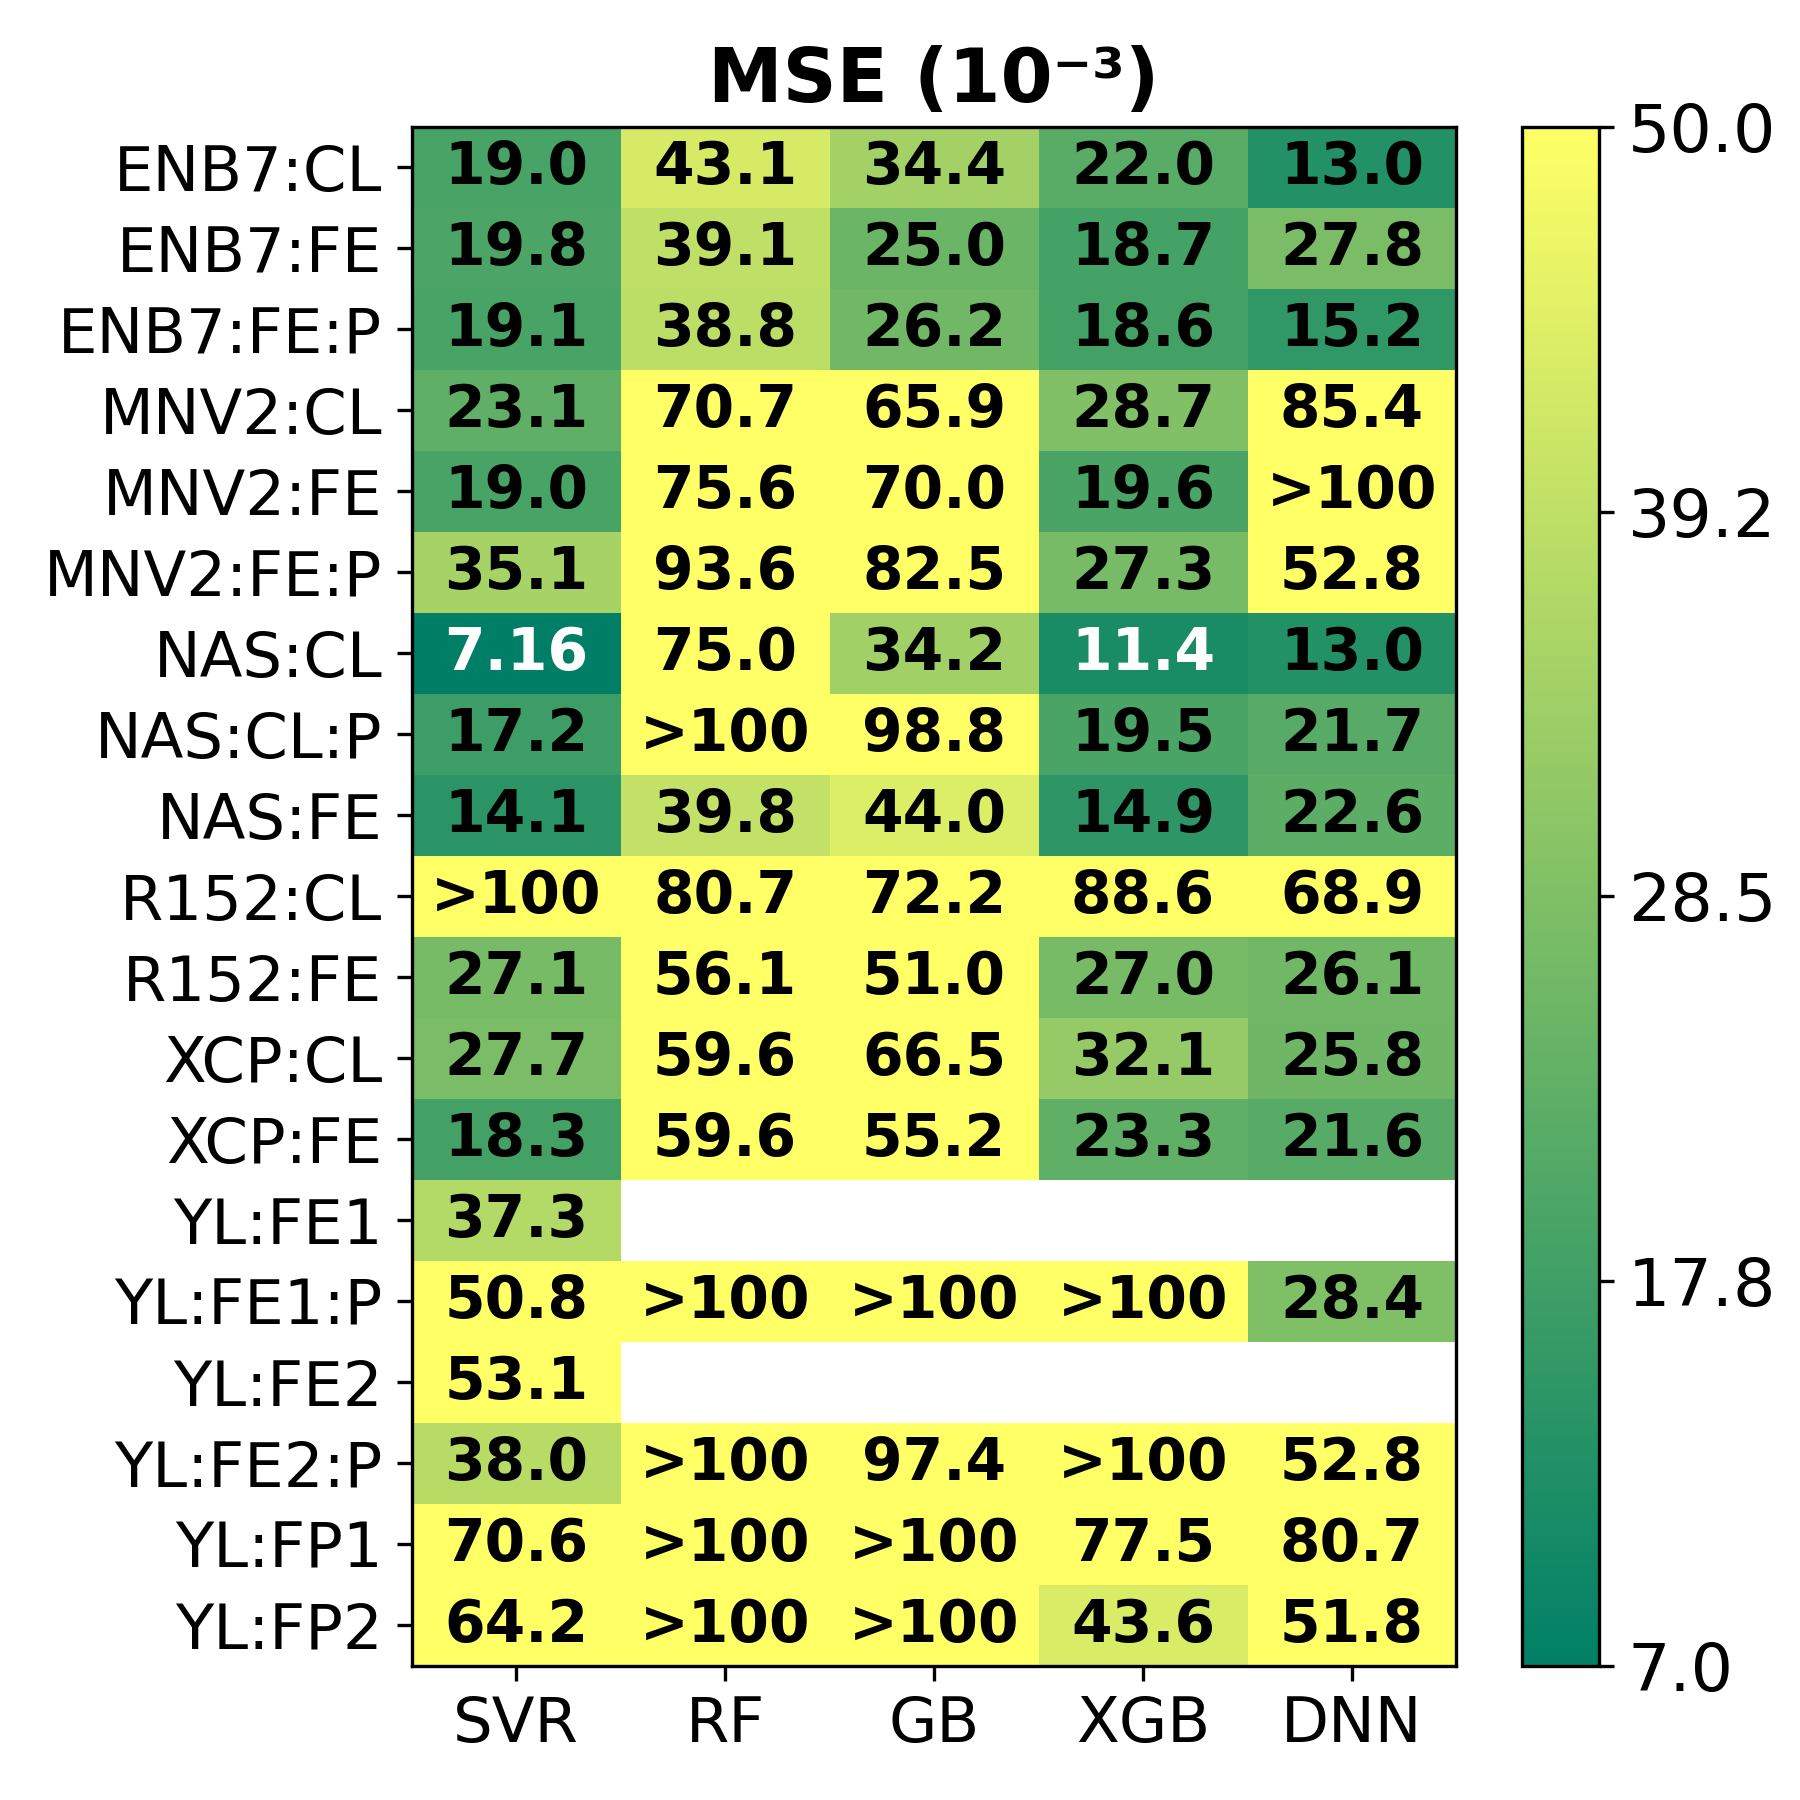
\includegraphics[width=0.35\textwidth]{Fig10a}
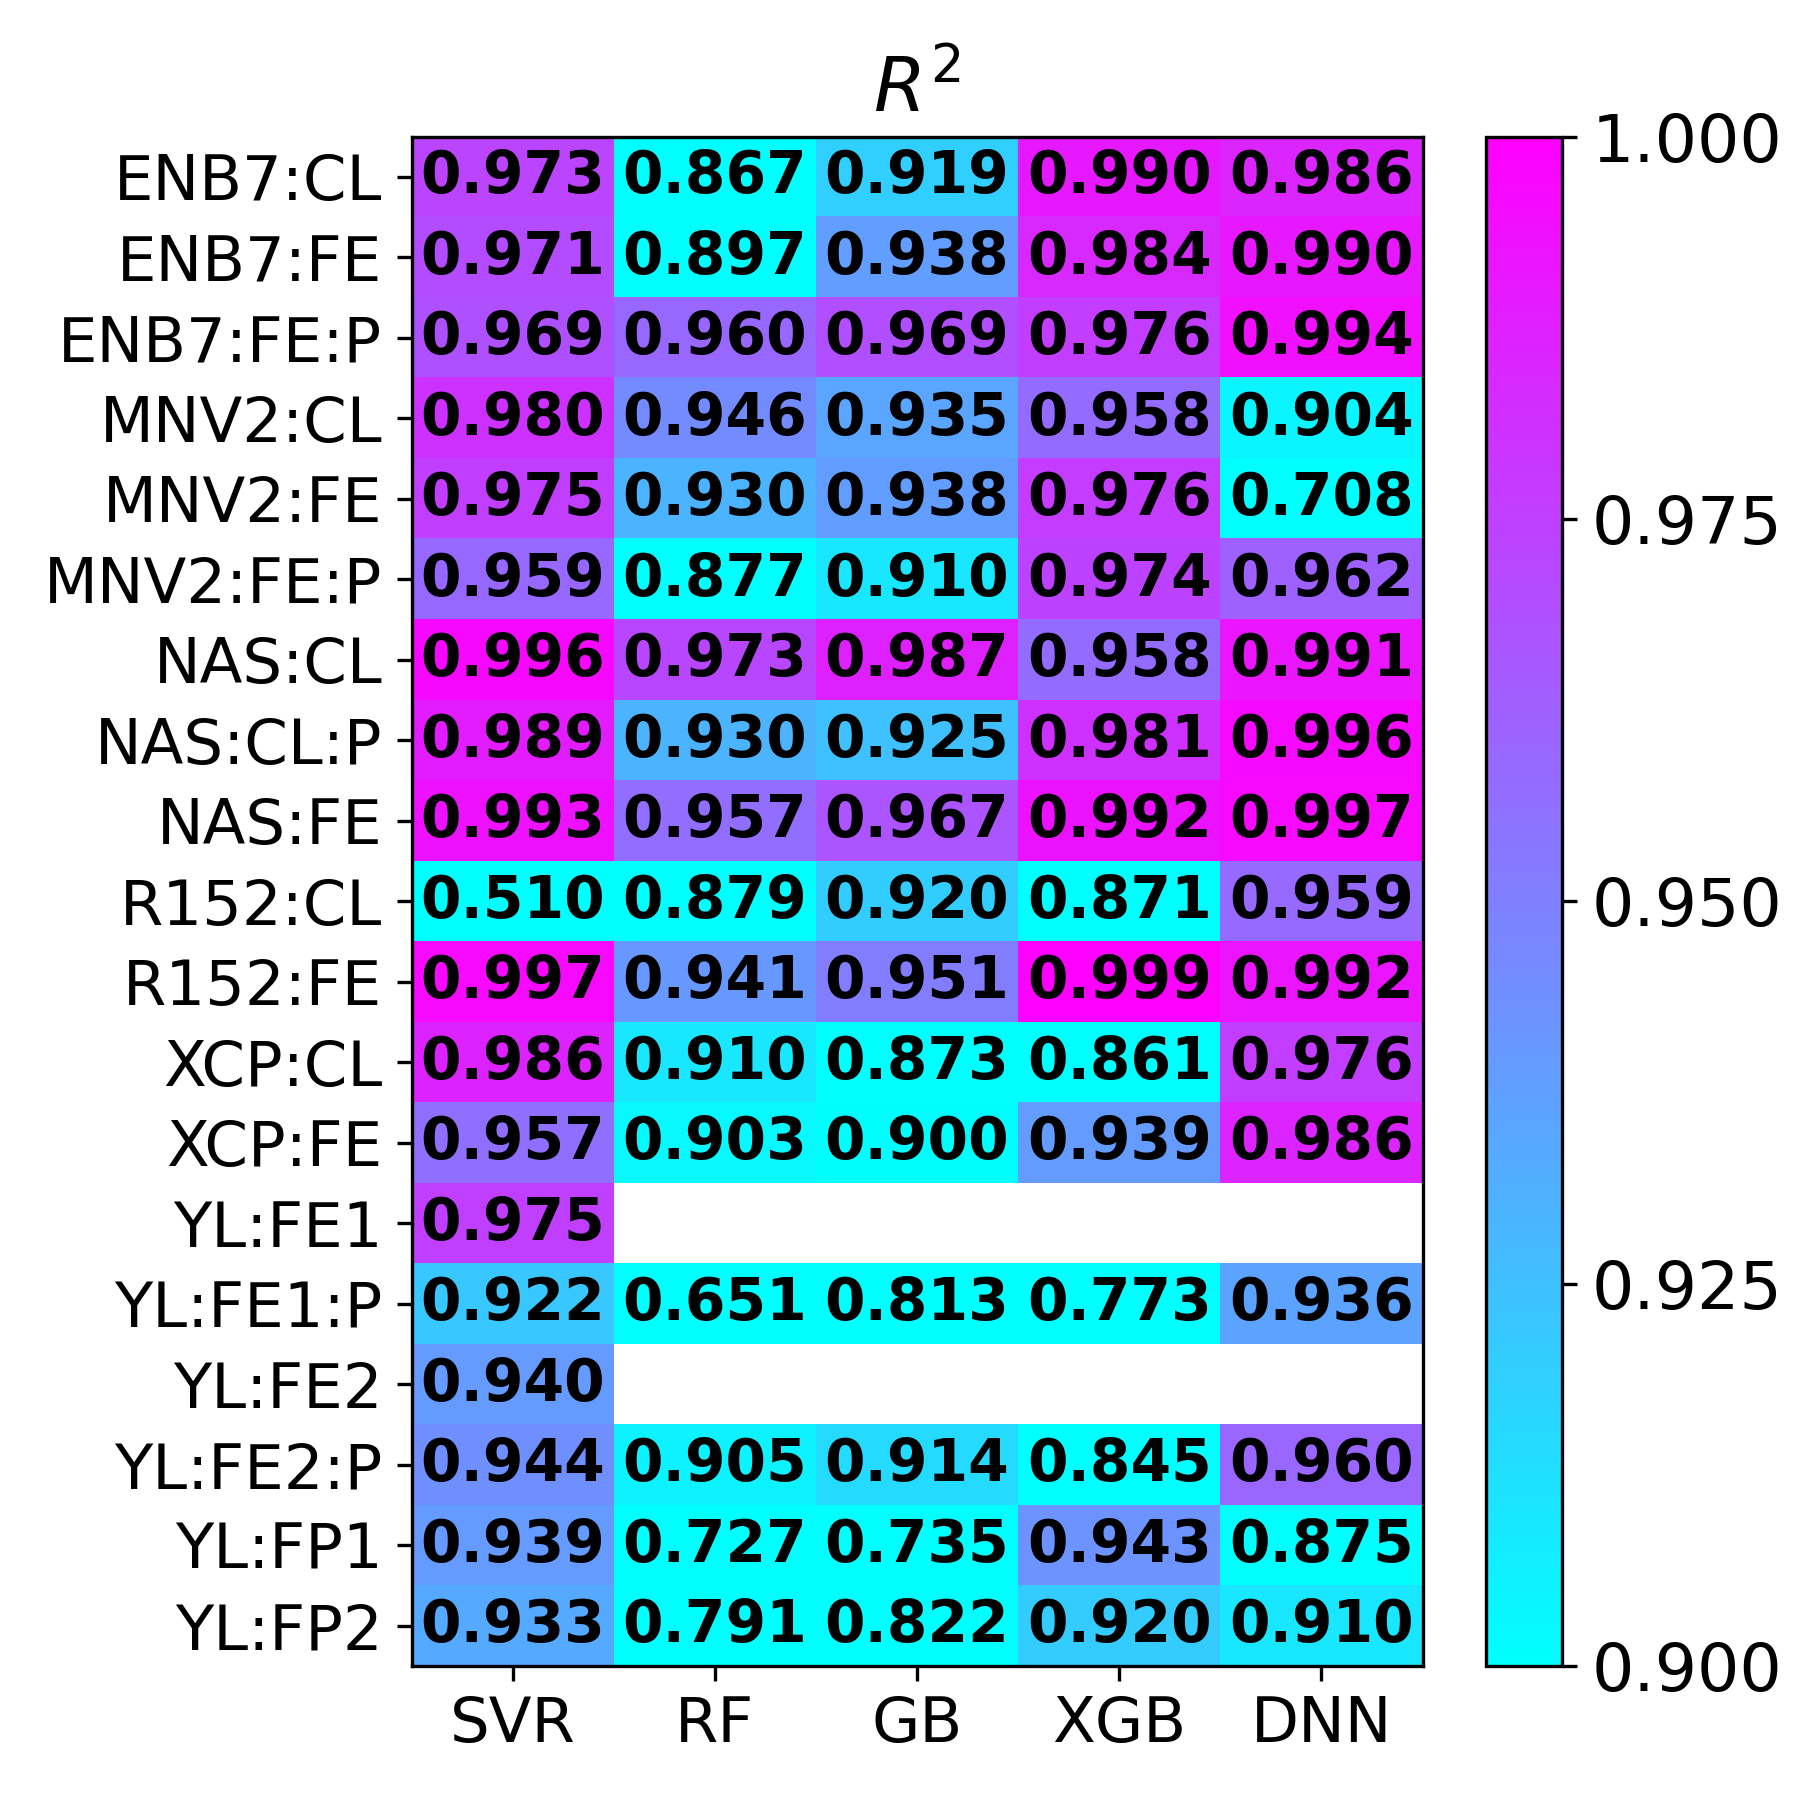
\includegraphics[width=0.35\textwidth]{Fig10b}
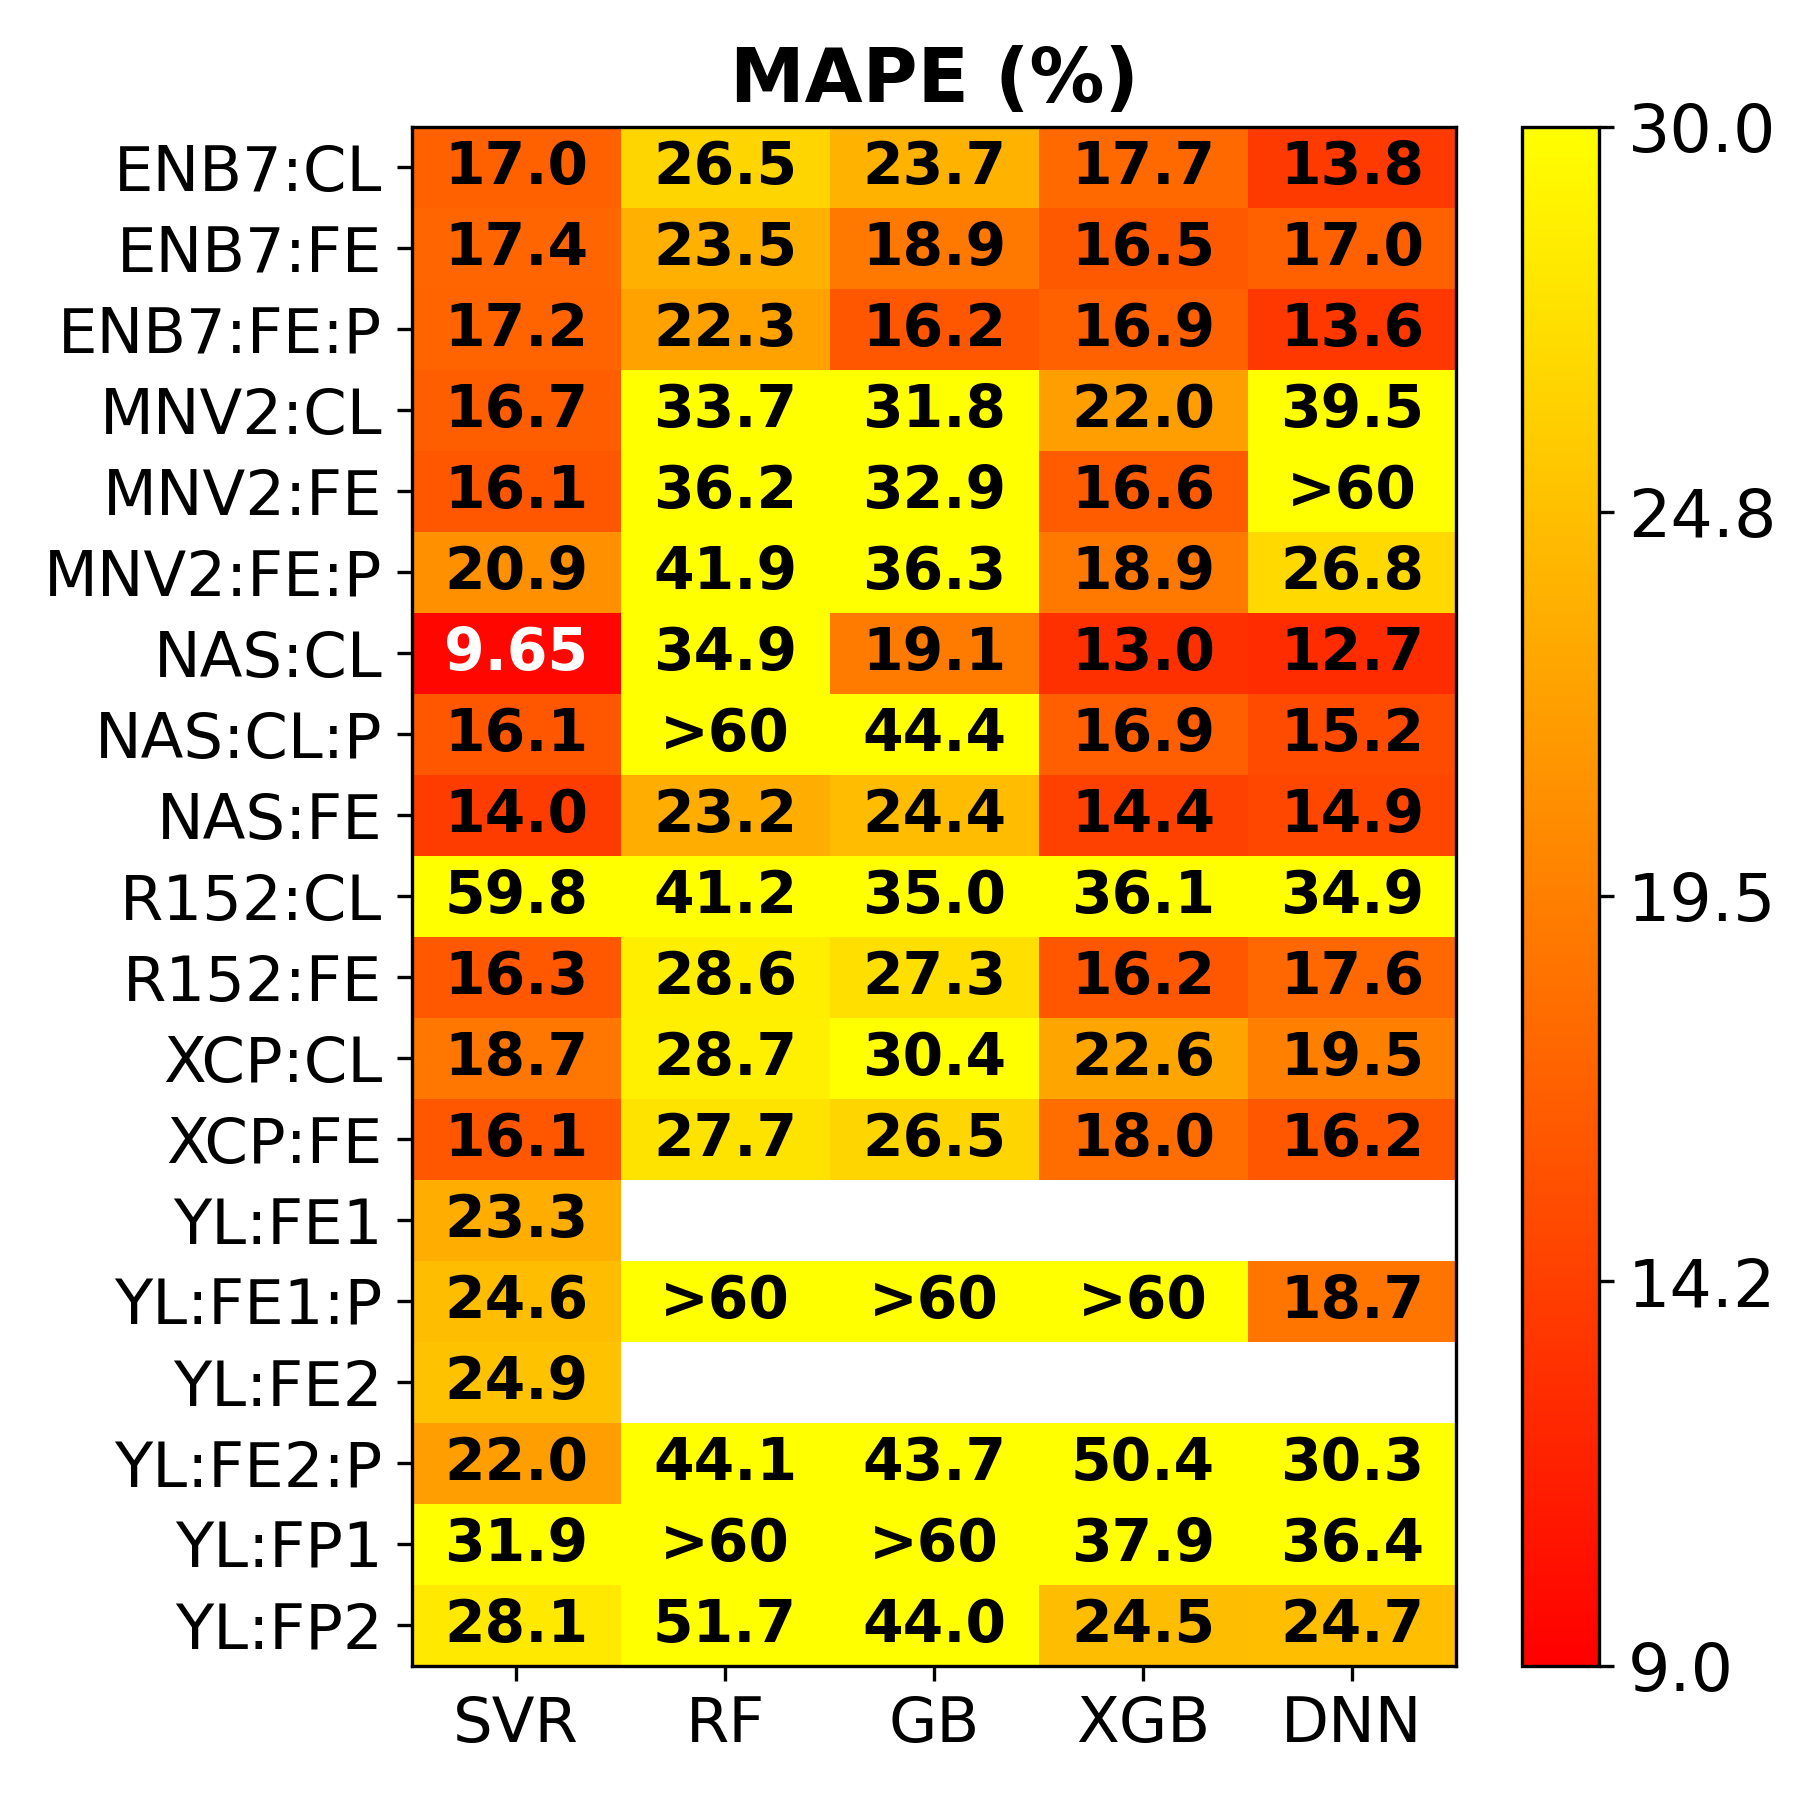
\includegraphics[width=0.35\textwidth]{Fig10c}
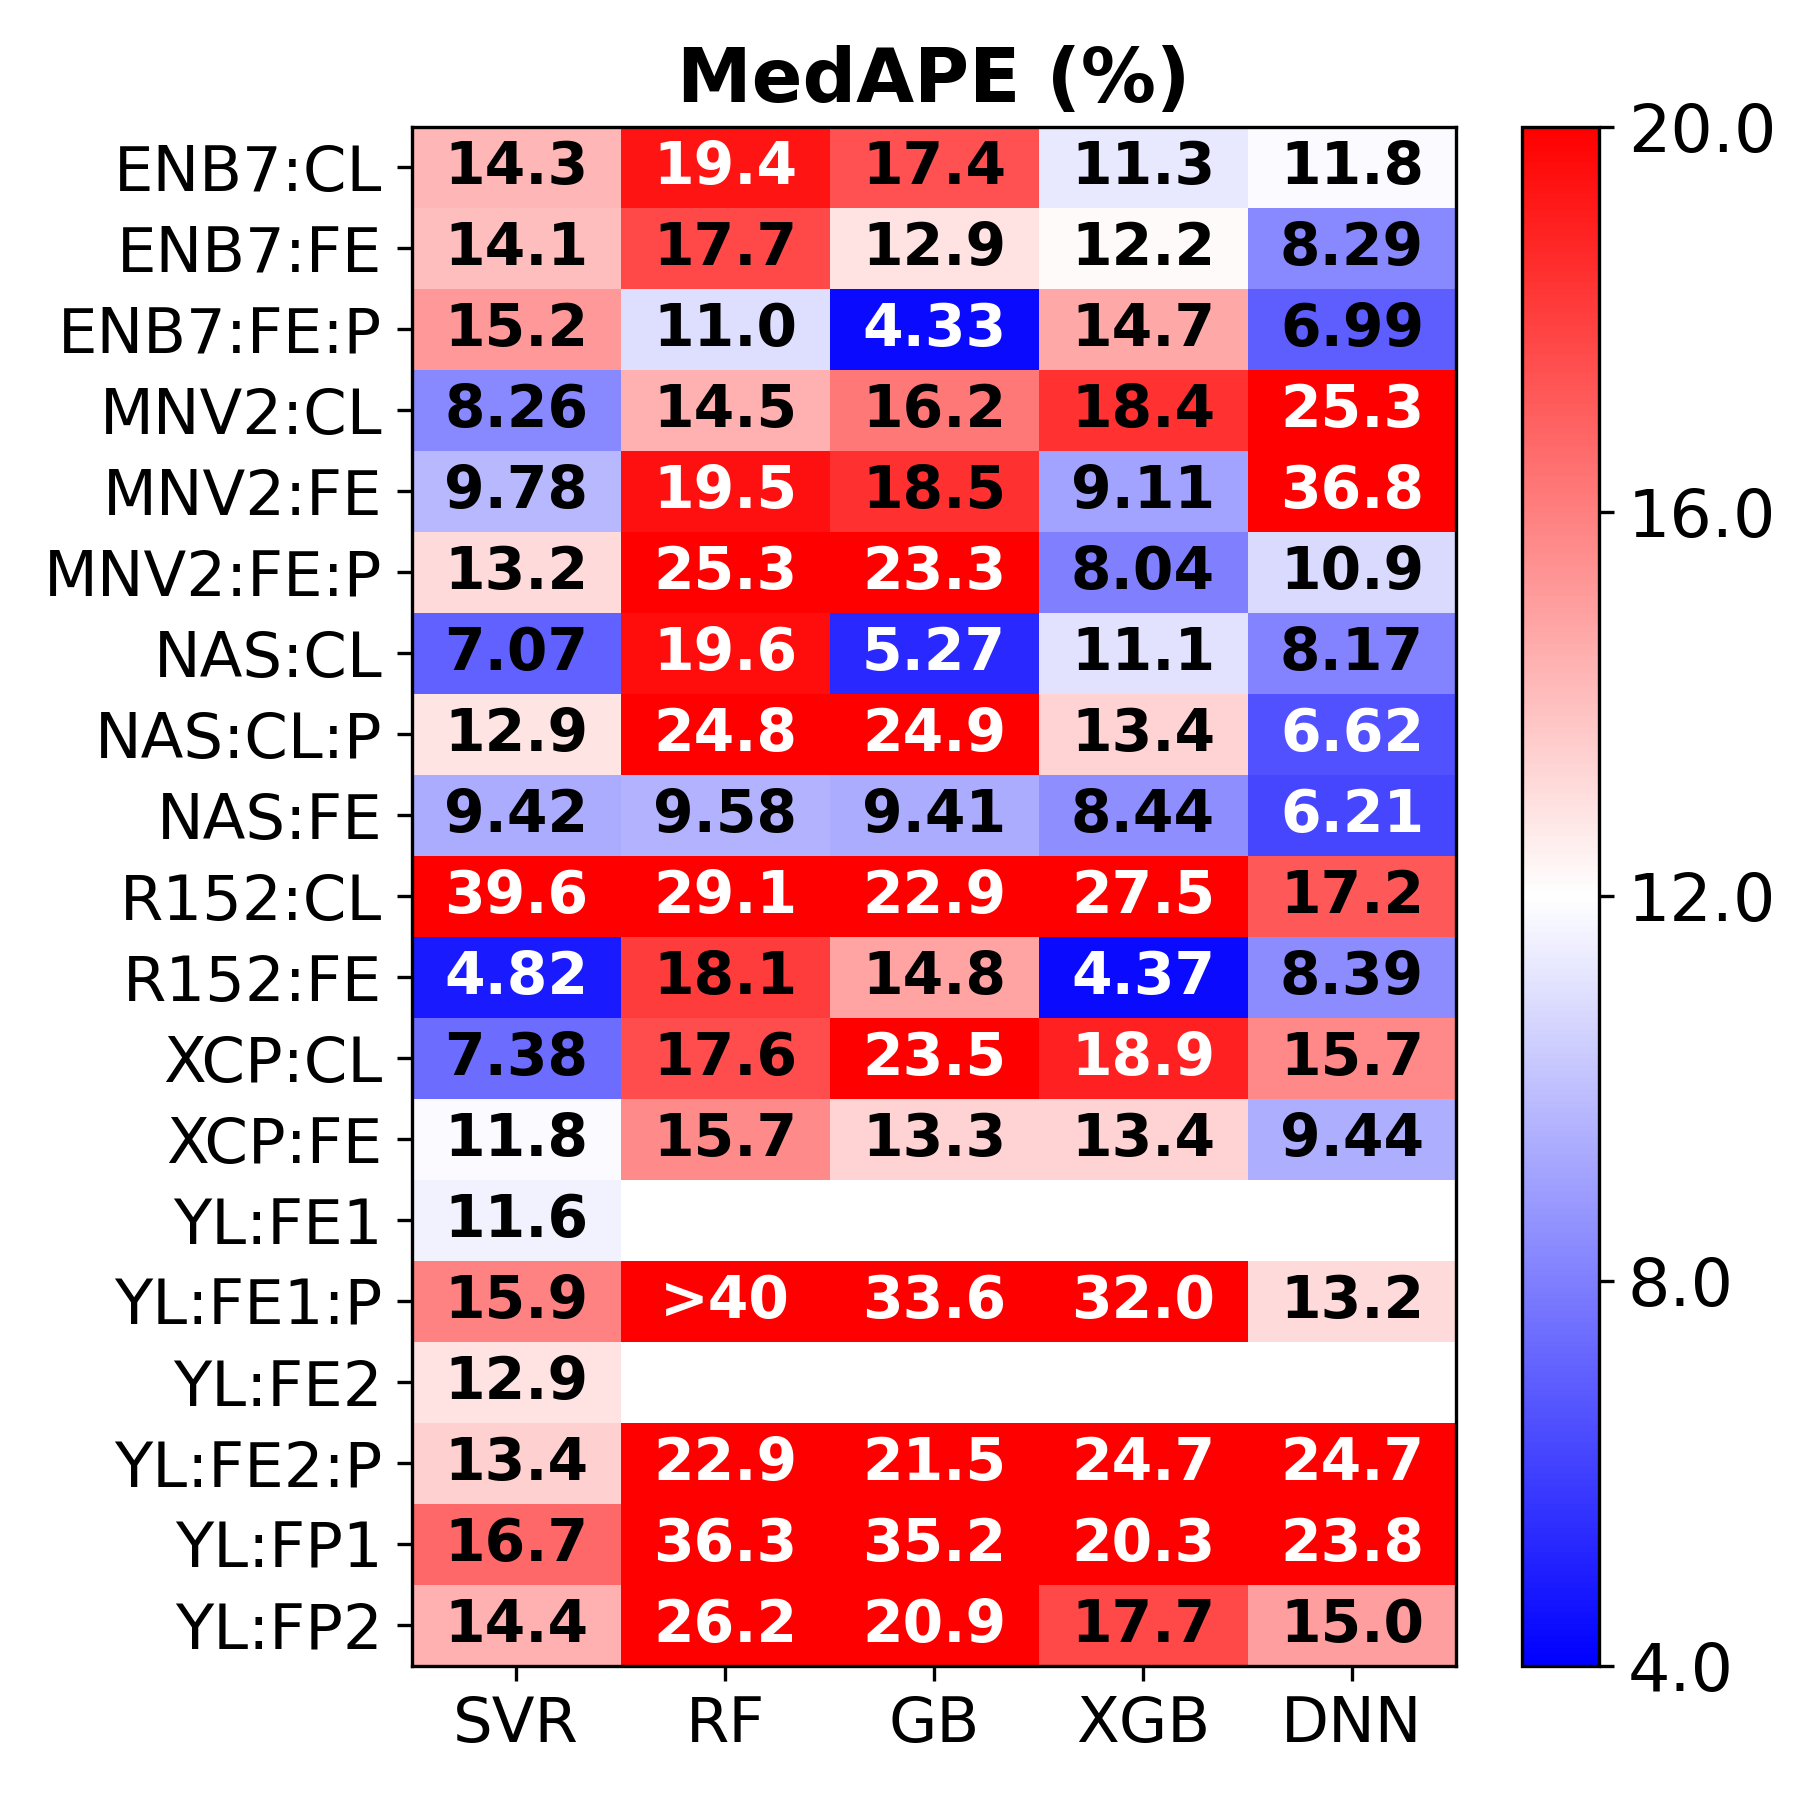
\includegraphics[width=0.35\textwidth]{Fig10d}
\caption{
Mean squared error, coefficient of determination, mean absolute percentage error, and median absolute percentage error
for different combinations of CV models (vertical axis) and regression models (horizontal axis)
during the test phase.
The models were trained on an experimental dataset.
}\label{Fig10}
\end{figure*}

In summary, three approaches for predicting iron concentrations from experimental data were evaluated:
(i)~models trained on simulated data,
(ii)~models trained on simulated data with post-hoc correction,
and (iii)~models trained directly on experimental data.
Training on simulated data alone yielded moderate agreement with experimental measurements,
but systematic biases were observed due to differences between the synthetic and real systems.
Post-hoc correction effectively reduced these biases, lowering the mean and median errors,
yet the correlation with the actual variation remained limited.
Direct training on experimental data provided the most balanced outcome,
achieving both low prediction errors and high correlation coefficients,
thereby demonstrating the importance of incorporating real measurements during model development.
Thus, training directly on experimental data improves prediction accuracy and eliminates the systematic biases observed in models transferred from synthetic data.
At the same time, achieving optimal performance requires both the careful selection of the CV model–regressor combination and the inclusion of real experimental data.


\section{Conclusion}

This study demonstrates that Transfer Learning from pretrained Computer Vision (CV) models enables accurate regression modeling 
even with the extremely small training datasets typical of experimental materials research. 
The proposed workflow involves measuring a characteristic kinetic dependency, 
transforming it into an image via wavelet analysis, 
extracting features using a pretrained CV model, 
and training a regression model on these features to predict material properties. 
The feasibility of this approach is illustrated by predicting the iron impurity concentration in silicon solar cell 
from short-circuit current kinetics following FeB pair dissociation using a training dataset of only 20–25 samples.

The performance of models trained on both synthetic and experimental datasets was evaluated. 
In both cases, EfficientNetB7 and NASNetLarge provided the most informative features, 
while Deep Neural Networks  and  Support Vector Regression yielded the highest prediction accuracy. 
The best-performing models achieved MSE, MAPE, MedAPE, and $R^2$ values of 0.001, 6\%, 4\%, and 0.999 for synthetic data, 
and 0.008, 10\%, 5\%, and 0.996 for experimental data.

When training models on synthetic data, image feature vectors serve as the most suitable descriptors for the regression model. 
In contrast, when experimental data are used, prediction accuracy can be improved and the influence of noise reduced 
by utilizing class probability distributions or applying Principal Component Analysis.

The combination of Transfer Learning from CNNs with an appropriate choice of descriptor type 
and regression algorithm represents a promising strategy for materials research in general 
and for defect characterization in particular, 
especially when the acquisition of large datasets is difficult or impractical.

\section*{References}

\bibliographystyle{iopart-num}
\bibliography{olikh}

\end{document}

